%!TEX program = lualatex
%!TEX encoding = UTF-8 Unicode  
%!TEX root = chapter05.tex  
\documentclass[main.tex]{subfiles} 
\begin{document} 
%----------------------------------------------------------------------------------------
%	CHAPTER 5
%----------------------------------------------------------------------------------------
\newpage 
\loadgeometry{marginlayout}  
\pagestyle{scrheadings} % Print headers again  
\KOMAoptions{
	headwidth=textwithmarginpar,
	headsepline=true,
	headsepline= 0.5pt,
	footwidth=textwithmarginpar,
}  
\onehalfspacing 
\setcounter{chapter}{4}
\chapter{Suites}  
\section{Définitions}
\begin{example}\sidenote{correspond aux chapitres 5, 8 et 10}\hfill
	\begin{enumerate}[label=\textbullet,leftmargin=*]
		\item La suite des nombres entiers $0; 1 ; 2 ; 3 \ldots$.
		\item La suite des nombres pairs $0; 2; 4; 6 ;\ldots$.
		\item La suite de Golomb (ou Silverman) : $1;2;2;3;3;3;4;4;4;4;5;5;5;5;5;\ldots$
		\item La suite \emph{look-and-say} de Conway $1;11;21;1211;111221;312211\ldots$
%		\item La suite $1;0;2;0;3;0;4;0;5;0;\ldots$.
%		\item La suite de 0 et de 1 : $0;1;0;0;1;1;1;0;1;0;1;1;0;\ldots$.
%		\item La suite de 0 et de 1 qui se repètent : $0;1;0;1;0;1;0;1;0;1;\ldots$.
%		\item La suite de 0 et de 1 : $1;0;1;0;0;1;0;0;0;1;0;0;0;0;1;\ldots$.
	\end{enumerate}
\end{example}  
\begin{definition} 
	Une suite numérique $u$ est une fonction définie sur $\mathbb{N}$ 
	\setlength{\abovedisplayskip}{3pt}
	\setlength{\belowdisplayskip}{3pt}
	$$\begin{aligned}[t]
		u : \mathbb{N} & \rightarrow \mathbb{R}   	\\
		n & \mapsto u(n)=u_n
		\end{aligned}
	$$
\noindent	Les antécédents $n$ sont appelés les \textbf{rangs} (ou les indices) des termes.

\noindent	Les images $u(n)$ sont  les \textbf{termes} de la suite et se notent aussi $u_n$ (on lit \og $u$ indice $n$\fg{}). 
\noindent	On note la suite $(u_n)_{n\in\mathbb{N}}$ ou simplement $(u_n)$.
\end{definition}  
On peut représenter une suite $(u_n)$ par un nuage de points de coordonnées $(n;u_n)$, où $n\in \mathbb{N}$. 
\begin{figure*}[!h]    
		\begin{tikzpicture}[xscale=1, yscale=0.35] 
			\tkzInit[xmin=0.0,xmax=10.0,ymin=0.0,ymax=9,xstep=1.0, ystep=1.0]; 
			\tkzDrawX[above=5pt, label={$x$}, font=\small, line width=1.2pt] 
			\tkzDrawY[right=5pt, label={$y$}, font=\small, line width=1.2pt]
			\tkzLabelX[orig=false,below=5pt,   font=\scriptsize, line width=1.2] 
			\tkzLabelY[orig=false,left=5pt,  font=\scriptsize, line width=1.2]   
			\draw (0,3) node[draw,thick,cross out] {}; 
			\draw (1,1) node[draw,thick,cross out] {}; 
			\draw (2,4) node[draw,thick,cross out] {}; 
			\draw (3,1) node[draw,thick,cross out] {}; 
			\draw (4,5) node[draw,thick,cross out] {}; 
			\draw (5,9) node[draw,thick,cross out] {}; 
			\draw (6,2) node[draw,thick,cross out] {}; 
			\draw (7,6) node[draw,thick,cross out] {}; 
			\draw (8,5) node[draw,thick,cross out] {}; 
			\draw (9,3) node[draw,thick,cross out] {}; 
			\draw (10,5) node[draw,thick,cross out] {};  
		\end{tikzpicture} 
	\caption{ 
		On considère la suite $(u_n)$ des décimales de $\pi\approx 3,14159265358979323846264338327950288419716939937510\ldots$ : $u_0=3$, $u_1=1$, $u_2=4\ldots$}
\end{figure*}
\begin{cBox}
	\noindent En général  une suite $(u_n)$ peut-être définie :
	\begin{itemize}
		\item de manière explicite : $u_n =f(n)$
		\item de manière récurrente : $\begin{cases}u_0 \\ u_{n+1} =f(u_n)\end{cases}$
	\end{itemize} 
\end{cBox}
%----------------------------------------------------------------------------------------
% 
%----------------------------------------------------------------------------------------
\newpage 
\loadgeometry{widelayout}  
\pagestyle{scrheadings} % Print headers again  
\KOMAoptions{
	headwidth=textwithmarginpar,
	headsepline=true,
	headsepline= 0.5pt,
	footwidth=textwithmarginpar,
}  
\onehalfspacing    
\subsection{Applications : estimer des solutions d'équations cubiques par itération}
\begin{example}On cherche à résoudre $x^3-10x =30$, inconnue $x$.
\end{example}
\begin{spacing}{2}
\noindent
\parbox{0.48\linewidth}{
Une solution $x^*$ vérifie  
$\begin{WithArrows}
	x^3-10x&=30\\
	x^3&=10x+30   	\\
	x& =  \sqrt[3]{10x+30} 
\end{WithArrows}$ 

Nous allons construire une suite de nombres qui se rapproche de $x^*$ par itération :
%\setlength{\abovedisplayskip}{3pt}
%\setlength{\belowdisplayskip}{3pt}
$ 
x_{n+1}=\sqrt[3]{10x_n+30}
$ 
}
\hfill 
\parbox{0.48\linewidth}{
	Une solution $x^*$ vérifie  
	$\begin{WithArrows} 
		x^3&=10x+30   	\\ 
		x^2& = 10 + \frac{30}{x}\\
		x& = \sqrt{10+\frac{30}{x}}
	\end{WithArrows}$ 
	
Nouveau itération possible :
\setlength{\abovedisplayskip}{3pt}
\setlength{\belowdisplayskip}{3pt}
$$
x_{n+1}=\sqrt{10+\frac{30}{x_n}}
$$
}
\end{spacing} 


\noindent
\parbox{0.24\linewidth}{
$\begin{cases}
	x_0=4  \\ 
	x_{n+1}=\sqrt[3]{10x_n+30}
\end{cases}$  
\begin{spacing}{2}
	\begin{enumerate}[leftmargin=*, label={},]
		\item $x_0=4$
		\item $x_1= $
		\item $x_2= $
		\item $x_3= $
%		\item $x_4= $
		\item $x_5= $ 
%		\item $x_9= $ 
		\item $x_{10}= $
	\end{enumerate}
\end{spacing} 
}
%\hfill 
\parbox{0.24\linewidth}{
$\begin{cases}
	x_0=5  \\ 
	x_{n+1}=\sqrt[3]{10x_n+30}
\end{cases}$  
\begin{spacing}{2}
	\begin{enumerate}[leftmargin=*, label={},]
		\item $x_0=5$
		\item $x_1= $
		\item $x_2= $
		\item $x_3= $
%		\item $x_4= $
		\item $x_5= $ 
%		\item $x_9= $ 
		\item $x_{10}= $
	\end{enumerate}
\end{spacing} 
}
%\hfill 
\parbox{0.24\linewidth}{
	$\begin{cases}
		x_0=4  \\ 
		x_{n+1}=\sqrt{10+\frac{30}{x_n}}
	\end{cases}$  
	\begin{spacing}{2}
		\begin{enumerate}[leftmargin=*, label={},]
			\item $x_0=4$
			\item $x_1= $
			\item $x_2= $
			\item $x_3= $
%			\item $x_4= $
			\item $x_5= $ 
%			\item $x_9= $ 
			\item $x_{10}= $
		\end{enumerate}
	\end{spacing} 
}
%\hfill 
\parbox{0.24\linewidth}{
	$\begin{cases}
		x_0=5  \\ 
		x_{n+1}=\sqrt{10+\frac{30}{x_n}}
	\end{cases}$  
	\begin{spacing}{2}
		\begin{enumerate}[leftmargin=*, label={},]
			\item $x_0=5$
			\item $x_1= $
			\item $x_2= $
			\item $x_3= $
%			\item $x_4= $
			\item $x_5= $ 
%			\item $x_9= $ 
			\item $x_{10}= $
		\end{enumerate}
	\end{spacing} 
}
\begin{spacing}{2}
\noindent Combien d'itérations $n$ avant que la valeur du terme $x_n$ semble se stabiliser ? \dotfill 

\noindent Il semble que pour $n$ suffisamment grand $x_n \approx $\dotfill $x_n \approx $\dotfill 

\noindent \emph{Cette valeur est appelée $\lim_{n\to\infty}x_n$, la limite de la suite $(x_n)_{n\in\mathbb{N}}$ quand $n$ tend vers $+\infty$.} 

\noindent Vérifier que la limite obtenue vérifie $\abs{x^3-10x-30}\leqslant 10^{-5}$. 
\end{spacing} 
\vspace{-1.0em}
\begin{example}[à vous] On cherche la solution de $x^3+2x =40$, inconnue $x$ sur l'intervalle $\interval{3}{4}$.
		\begin{enumerate}[leftmargin=*,label=\arabic*)]
		\item Montrer que la solution $x^*$ vérifie $x=\sqrt[3]{-2x+40}$ et $x=\sqrt{-2+\frac{40}{x}}$.
		\item Proposer deux approches différentes de résolution par itération. Choisissez une valeur initiale $x_0$ et la relation de récurrence. 
		\item Pour chaque approche :
		\begin{enumerate}[leftmargin=*,label=\alph*)]
			\item Calculer les premiers termes.
			\item Est ce que la suite $x_n$ semble se rapprocher d'une valeur $l$ ?  \\
			  Combien d'itérations sont nécessaires ? 
			\item Vérifier si $l$ est une valeur approchée d'une solution : $\abs{l^3+2l+40}\leqslant $  
			\item Laquelle des deux approches est plus rapide ?
		\end{enumerate}
	\end{enumerate}
\end{example}
\begin{exercise} Mêmes questions pour les solutions de cubiques suivantes.
\begin{multicols}{3}
	\begin{spacing}{2}
	\begin{enumerate}[leftmargin=*,label=\arabic*)]
		\item $x^3+10x=51$ sur $\interval{2}{3}$
		\item $x^3+2x=1$ sur $\interval{0}{1}$
		\item $x^3+4x=10$ sur $\interval{1}{2}$
		\item $x^3+10x=25$ sur $\interval{1}{2}$
		\item[\textbullet] $x^3-4x=10$ sur $\interval{2}{3}$
		\item[\textbullet] $x^3-3x=2$ sur $\interval{1}{3}$
	\end{enumerate} 
	\end{spacing}
\end{multicols}
\end{exercise}

\begin{exercise}[Rappels Python]\hfill 
	

\noindent
%\parbox{0.35\linewidth}{
\begin{minipage}{0.38\linewidth} 
\begin{lstlisting}[ language=python , 
	%	title=Script B,   
	linewidth=0.95\columnwidth,
	style=python-code,    
	aboveskip=0.0\topskip,
	belowskip=0.0\topskip,
	xleftmargin=1.2em,
	%	lineskip=1.0em,
	tabsize=4, 
	%numbers=none,
	%	firstnumber=10  
] 
def u(n) :
	nbr = 3
	for i in range(n) :
		nbr = nbr + 1
	return nbr
\end{lstlisting} 
\end{minipage} 
\hfill 
\parbox{0.6\linewidth}{
L'instruction \lstinline|u(5)| retourne \dotfill 
\begin{enumerate}[label=\ding{111}, leftmargin=*] 
	\item $3+1+1+1+1$
	\item $3+1+1+1+1+1$
	\item $3+1+1+1+1+1+1$
	\item $3+1+1+1+1+1+1+1$
\end{enumerate}
}

\noindent
%\parbox{0.35\linewidth}{
\begin{minipage}{0.38\linewidth} 
\begin{lstlisting}[ language=python , 
%	title=Script B,   
linewidth=0.95\columnwidth,
style=python-code,    
aboveskip=0.0\topskip,
belowskip=0.0\topskip,
xleftmargin=1.2em,
%	lineskip=1.0em,
tabsize=4, 
%numbers=none,
%	firstnumber=10  
] 
def v(n) :
	nbr = 10
	for i in range(n) :
	nbr = 2*nbr
	return nbr
\end{lstlisting} 
\end{minipage} 
\hfill 
\parbox{0.6\linewidth}{
L'instruction \lstinline|v(6)| retourne \dotfill 
\begin{enumerate}[label=\ding{111}, leftmargin=*] 
\item $10\times 2 \times 6$ 
\item $10\times 2 \times 2 \times 2 \times 2$ 
\item $10\times 2 \times 2 \times 2 \times 2\times 2$ 
\item $10\times 2 \times 2 \times 2 \times 2\times 2\times 2$ 
\end{enumerate}
}


\noindent
%\parbox{0.35\linewidth}{
\begin{minipage}{0.38\linewidth} 
\begin{lstlisting}[ language=python , 
%	title=Script B,   
linewidth=0.95\columnwidth,
style=python-code,    
aboveskip=0.0\topskip,
belowskip=0.0\topskip,
xleftmargin=1.2em,
%	lineskip=1.0em,
tabsize=4, 
%numbers=none,
%	firstnumber=10  
] 
def w(n) :
	nbr = 3
	for i in range(1,n) :
		nbr = i*nbr
	return nbr
\end{lstlisting} 
\end{minipage} 
\hfill 
\parbox{0.6\linewidth}{
L'instruction \lstinline|w(5)| retourne \dotfill 
\begin{enumerate}[label=\ding{111}, leftmargin=*] 
\item $3\times 5$ 
\item $3\times 1 \times 2 \times 3  $ 
\item $3\times 5 \times 5 \times 5 \times 5  $ 
\item $3\times 1 \times 2 \times 3 \times 4$ 
\end{enumerate}
}

\noindent
%\parbox{0.35\linewidth}{
\begin{minipage}{0.38\linewidth} 
\begin{lstlisting}[ language=python , 
%	title=Script B,   
linewidth=0.95\columnwidth,
style=python-code,    
aboveskip=0.0\topskip,
belowskip=0.0\topskip,
xleftmargin=1.2em,
%	lineskip=1.0em,
tabsize=4, 
%numbers=none,
%	firstnumber=10  
] 
def f(n) :
	nbr = 0
	for i in range(1,n+1) :
		nbr = i^2 + nbr
	return nbr
\end{lstlisting} 
\end{minipage} 
\hfill 
\parbox{0.6\linewidth}{
L'instruction \lstinline|f(5)| retourne \dotfill 
\begin{enumerate}[label=\ding{111}, leftmargin=*] 
\item $2 \times 5^2$ 
\item $0+ 1^2 +2^2+3^2+4^2  $ 
\item $0+ 1^2 +2^2+3^2+4^2 + 5^2 $ 
\item $0+ 1^2 +2^2+3^2+4^2 + 5^2 + 6^2$ 
\end{enumerate}
} 
\end{exercise}
\begin{exercise} En vous aidant du tableau, préciser ce qu'affiche les scripts suivants :\hfill

\noindent\begin{minipage}{0.25\columnwidth}
\begin{lstlisting}[ language=python , 
%	title=Script B,   
linewidth=1\columnwidth,
style=python-code,    
aboveskip=0.0\topskip,
belowskip=0.0\topskip,
xleftmargin=1.2em,
%	lineskip=1.0em,
tabsize=4, 
%	numbers=none,
%	firstnumber=10  
] 
n , nbr = 0 , 1
while nbr > 0.5 :
	n = n+1
	nbr = 0.88*nbr
print(n)
\end{lstlisting} 
\end{minipage}
\begin{minipage}{0.75\columnwidth} 
\begin{tabularx}{0.98\linewidth}{|c|*{7}{>{\centering \arraybackslash}X|}}\hline
\rule[-0.6em]{0em}{1.8em}		\lstinline|n|  &   $1$ &   $2$& $3$ & $4$ & $5$  & $6$& $7$   \\ \hline
\rule[-0.6em]{0em}{3.2em}	\lstinline|nbr|      &   &&&   &&&  \\ \hline
\end{tabularx}  
\end{minipage}

\begin{multicols}{2}
\begin{enumerate}[label=\ding{111}, leftmargin=*]
\item 6
\item 5
\item Le plus petit entier $n$ tel que $0.88^{n}\geqslant 0.5$
\item Le plus petit entier $n$ tel que $0.88^{n}\leqslant 0.5$
\item Rien car il ne s'arrête pas 
\item 0.464404
\end{enumerate}		
\end{multicols} 

\noindent\begin{minipage}{0.25\columnwidth}
\begin{lstlisting}[ language=python , 
%	title=Script B,   
linewidth=1\columnwidth,
style=python-code,    
aboveskip=0.0\topskip,
belowskip=0.0\topskip,
xleftmargin=1.2em,
%	lineskip=1.0em,
tabsize=4, 
%	numbers=none,
%	firstnumber=10  
] 
n , nbr = 0 , 1
while nbr < 2 :
	n = n+1
	nbr = 1.15*nbr
print(n) 
\end{lstlisting} 
\end{minipage}
\begin{minipage}{0.75\columnwidth} 
\begin{tabularx}{0.98\linewidth}{|c|*{7}{>{\centering \arraybackslash}X|}}\hline
\rule[-0.6em]{0em}{1.8em}		\lstinline|n|  &   $1$ &   $2$& $3$ & $4$ & $5$  & $6$& $7$    \\ \hline
\rule[-0.6em]{0em}{3.2em}	\lstinline|nbr|      &   &&&   &&&  \\ \hline
\end{tabularx}  
\begin{multicols}{2}
\begin{enumerate}[label=\ding{111}, leftmargin=*] 
	\item 5
	\item \small Le plus petit entier $n$ tel que $1.15^{n}\geqslant 2$ 
	\item Rien car il ne s'arrête pas 
	\item \numprint{2.0113572}
\end{enumerate}		
\end{multicols} 
\end{minipage}


\end{exercise}  
%----------------------------------------------------------------------------------------
%	CHAPTER 5
%----------------------------------------------------------------------------------------
\newpage 
\loadgeometry{marginlayout}  
\pagestyle{scrheadings} % Print headers again  
\KOMAoptions{
	headwidth=textwithmarginpar,
	headsepline=true,
	headsepline= 0.5pt,
	footwidth=textwithmarginpar,
}  
\onehalfspacing  
\section{Etude d'une suite}
 
 \begin{definition} Soit la suite $u=(u_n)_{n\in\mathbb{N}}$ \\
$u$ est \textbf{croissante} (à partir du rang $N$) lorsque :
 	\setlength{\abovedisplayskip}{3pt}
 	\setlength{\belowdisplayskip}{3pt}
 	\[
 	\text{pour tout $n\geqslant N$} \qquad u_{n+1}\geqslant u_n
 	\]
$u$ est \textbf{décroissante} (à partir du rang $N$) lorsque :
 	\setlength{\abovedisplayskip}{3pt}
 	\setlength{\belowdisplayskip}{3pt}
 	\[
 	\text{pour tout $n\geqslant N$} \qquad u_{n+1}\leqslant u_n
 	\] 
\end{definition}

\paragraph{Méthode \no 1}  
\noindent Si pour $n\geqslant N$ on a $u_{n+1}-u_n\geqslant 0$, la suite $(u_n)$ est croissante ! \sidenote{La suite $v=(v_n)_{n\in\mathbb{N}}$ définie par $v_n=u_{n+1}-u_n$ est la suite dérivée de la suite $(u_n)$.}

\paragraph{Méthode \no 2} valable uniquement si la suite $(u_n)$ a des termes \textbf{strictement positifs}.

\noindent Si pour tout $n\geqslant N$ , le ratio $\frac{u_{n+1}}{u_n}\geqslant 1$, la suite $u$ est croissante.

\begin{remark} méthode 2 est conséquence de  1 : $\frac{u_{n+1}}{u_n}-  1=\frac{u_{n+1}-u_n}{u_n}$. 
	
\end{remark} 
\paragraph{Méthode \no 3} Si l'on connait l'expression explicite de la suite $u$ : $u_n=f(n)$, le sens de variation de $u$ est celui  de $f$ sur $\interval[open right]{0}{+\infty}$.
\begin{example}Montrer les méthodes sur l'exemple $u_n=\frac{1}{3n+2}$
	\end{example}
\paragraph{Notion intuitive de limite} Pas de définition précise.

 On dira qu'une suite $u$ \textbf{converge vers $l$} si ses termes, à partir d'un certain rang, se rapprochent de $l$. On écrit $\lim_{n\to\infty}u_n=l$.

On dira qu'une suite $u$ \textbf{diverge vers $+\infty$} si pour tout réel $A$, les termes dépassent $A$ à partir d'un certain rang. On écrit $\lim_{n\to\infty}u_n=+\infty$.
\begin{figure*}[!h]
%	Si $-1<q<0$, alors $q^n$ n'est ni croissant ni décroissant,\\
%	et $\lim\limits_{n\to+\infty}q^n =0$ 
	\begin{tikzpicture}[xscale=0.5, yscale=1] 
		\tkzInit[xmin=-0.0,xmax=10.0,ymin=-1.0,ymax=2,xstep=1, ystep=1];
		%	\tkzGrid(0,-4)(10,4);  
		\tkzDrawX[above=5pt, label={$x$}, font=\small, line width=1.2pt] 
		\tkzDrawY[right=5pt, label={$y$}, font=\small, line width=1.2pt]
		\tkzLabelX[orig=false,below=5pt,   font=\scriptsize, line width=1.2] 
		\tkzLabelY[orig=false,left=5pt,  font=\scriptsize, line width=1.2]  
		\tkzSetUpPoint[size=3, fill=black]
		\global\edef\tkzFctLast{1*(-0.65)^x+1}
		\foreach \va in {0,1,...,10}{%
			\tkzDefPointByFct[draw](\va)}
		%	\tkzDrawPoints(A0,A1, A2,A3,A4,A5);   
		\tkzHLine[color=red]{1} 
	\end{tikzpicture}
	\begin{tikzpicture}[xscale=0.5, yscale=1] 
	\tkzInit[xmin=-0.0,xmax=10.0,ymin=-1.0,ymax=2,xstep=1, ystep=1];
	%	\tkzGrid(0,-4)(10,4);  
	\tkzDrawX[above=5pt, label={$x$}, font=\small, line width=1.2pt] 
	\tkzDrawY[right=5pt, label={$y$}, font=\small, line width=1.2pt]
	\tkzLabelX[orig=false,below=5pt,   font=\scriptsize, line width=1.2] 
	\tkzLabelY[orig=false,left=5pt,  font=\scriptsize, line width=1.2]  
	\tkzSetUpPoint[size=3, fill=black]
	\global\edef\tkzFctLast{0.2*(-1.2)^x+1}
	\foreach \va in {0,1,...,10}{%
		\tkzDefPointByFct[draw](\va)}
	%	\tkzDrawPoints(A0,A1, A2,A3,A4,A5);   
	\tkzHLine[color=red]{1} 
\end{tikzpicture}
	\begin{tikzpicture}[xscale=0.5, yscale=1] 
	\tkzInit[xmin=-0.0,xmax=10.0,ymin=-1.0,ymax=2,xstep=1, ystep=1];
	%	\tkzGrid(0,-4)(10,4);  
	\tkzDrawX[above=5pt, label={$x$}, font=\small, line width=1.2pt] 
	\tkzDrawY[right=5pt, label={$y$}, font=\small, line width=1.2pt]
	\tkzLabelX[orig=false,below=5pt,   font=\scriptsize, line width=1.2] 
	\tkzLabelY[orig=false,left=5pt,  font=\scriptsize, line width=1.2]  
	\tkzSetUpPoint[size=3, fill=black]
	\global\edef\tkzFctLast{0.2*(1.2)^x+1}
	\foreach \va in {0,1,...,10}{%
		\tkzDefPointByFct[draw](\va)}
	%	\tkzDrawPoints(A0,A1, A2,A3,A4,A5);   
%	\tkzHLine[color=red]{1} 
\end{tikzpicture}
\caption{Exemples de suites avec de gauche à droite : $\lim_{n\to\infty}u_n=1$, une suite sans limites, et une suite divergente vers $+\infty$ : $\lim_{n\to\infty}u_n=+\infty$}
\end{figure*}
%----------------------------------------------------------------------------------------
%	 
%----------------------------------------------------------------------------------------
\newpage 
\loadgeometry{widelayout}  
\pagestyle{scrheadings} % Print headers again  
\KOMAoptions{
	headwidth=textwithmarginpar,
	headsepline=true,
	headsepline= 0.5pt,
	footwidth=textwithmarginpar,
}  
\onehalfspacing  
\subsection{Exercices : définition de suites et sens de variation} 
\begin{exercise} En étudiant le signe de $u_{n+1}-u_n$, étudier les variations des suites $u$, définies pour tout   $n\in\mathbb{N}$.
		\begin{multicols}{4}
		\begin{spacing}{2} 
			\begin{enumerate}[label={\arabic*)$u_n=$}, leftmargin=*]
				\item $  n^2+2n$ 
				\item $  \dfrac{4}{n+1}$ 
				\item $ -5^n$ 
				\item $2^n-3$ 
			\end{enumerate} 
		\end{spacing}
	\end{multicols}  
\end{exercise} 
\begin{exercise}  En comparant $\dfrac{u_{n+1}}{u_{n}}$ avec $1$, étudier les variations des suites $u$, définies pour tout   $n\in\mathbb{N}$.
	\begin{multicols}{4}
		\begin{spacing}{2} 
			\begin{enumerate}[label={\arabic*)$u_n=$}, leftmargin=*]
				\item $ 7 \times 0,5^n$ 
				\item $  4 \times 9^n$ 
				\item $  \frac{2}{3^n}$ 
				\item $5\times \frac{2^n}{3^{n+1}}$  
			\end{enumerate} 
		\end{spacing}
	\end{multicols}  
\end{exercise}
\begin{exercise} Soit $u$ la suite définie pour tout entier $n \geqslant 1$ par $u_n = \dfrac{2^n}{n}$
	\begin{enumerate}[label={\arabic*)}, leftmargin=*]
		\item Calculer $\dfrac{u_{n+1}}{u_{n}}$
		\item Résoudre l'inéquation $\dfrac{2n}{n+1} > 1$
		\item En déduire les variations de la suite $(u_n)$.
	\end{enumerate} 
\end{exercise}
\begin{exercise}[entrainement] Étudier le sens de variation de la suite définie pour tout $n\geqslant 1$ par $u_n = \dfrac{\numprint{1.01}^n}{n}$ 
\end{exercise}
\begin{exercise}   Soit $u$ la suite définie pour tout entier $n \in\mathbb{N}$ par $u_n =2n^2-3n+1$
	\begin{enumerate}[label={\arabic*)}, leftmargin=*]
		\item Dresser le tableau de variation de la fonction quadratique définie sur $\mathbb{R}$ par $f(x)=2x^2-3x+1$.
		\item En déduire les variations de la suite $u$.
	\end{enumerate} 
\end{exercise}
\begin{exercise}[suites de la forme $u_n=f(n)$] \hfill \\
Étudier les variations des  suites $u$   définies pour tout entier $n \in\mathbb{N}$ par :
	\begin{multicols}{3}
	\begin{spacing}{2} 
		\begin{enumerate}[label={\arabic*)$u_n=$}, leftmargin=*]
			\item $n^2-10n+3$ 
			\item $n^3-n^2+n$ 
			\item $\sqrt{4n+6}$
			\item $7+\frac{5}{n}$
			\item $ \frac{n-3}{2n+1}$ 
			\item $  \frac{n}{n^2+1}$ 
		\end{enumerate} 
	\end{spacing}
\end{multicols}   
\end{exercise} 
%\begin{exercise} \hfill \\ Étudier les variations de la suite $u$   définie pour tout entier $n \in\mathbb{N}$   par $u_n =n^3-n^2+n$ 
%\end{exercise} 
%\begin{exercise} \hfill \\
%Étudier les variations de la suite $u$   définie pour tout entier $n \in\mathbb{N}$ par $u_n =\frac{n}{n^2+1}$ 
%\end{exercise} 
%\begin{exercise} \hfill \\
%	Étudier les variations de la suite $u$   définie pour tout entier $n \in\mathbb{N}$ par $u_n =\sqrt{4n+6}$ 
%\end{exercise}  
\begin{exercise}[suites définies par récurrence] Étudier les variations des suites ci-dessous.
\begin{enumerate}[label={\arabic*)}, leftmargin=*]
		\item $u_{n}$ définie par $u_0=3$ et  pour tout $n \in \mathbb{N}$, par $u_{n+1}=3u_n$
	\item $u_{n}$ définie par $u_0=3$ et  pour tout $n \in \mathbb{N}$, par $u_{n+1}=u_n+\sqrt{n}$
	\item $u_{n}$ définie par $u_0=-2$ et  pour tout $n \in \mathbb{N}$, par $u_{n+1}=u_n^2+u_n+2$
	\item $u_{n}$ définie par $u_0=3$ et pour tout $n \in \mathbb{N}$, par $u_{n+1}=\dfrac{3}{u_n}$ (\emph{exprimer $u_{n+2}$ à l'aide de $u_n$})
\end{enumerate} 
\end{exercise} 
\begin{exercise} À l'aide de la calculatrice, conjecturez la limite des suites $u$ définies par .
	\begin{multicols}{3}
	\begin{spacing}{2} 
		\begin{enumerate}[label={\arabic*)$u_n=$}, leftmargin=*]
			\item $-3n+5$ 
			\item $\left(-\frac{2}{3}\right)^n+5$ 
			\item $1.5^n-100$   
			\item $ \frac{1}{n}$  
			\item $ \frac{n+2}{2n-1}$  
			\item $ \frac{5n-2}{3n+1}$  
		\end{enumerate} 
	\end{spacing}
\end{multicols} 
\end{exercise}
\begin{exercise} À l'aide de la calculatrice, conjecturez la limite des suites suivantes.
	\begin{multicols}{2}
		\begin{spacing}{2} 
			\begin{enumerate}[label={\arabic*)$u_{n+1}=$}, leftmargin=*]
				\item $2u_n-6$, et $u_0=2$
				\item $\numprint{0.6}u_n+2$, et $u_0=1$
				\item $\frac{1}{u_n}$, et $u_0=5$
				\item $\frac{-1}{3}u_n$, et $u_0=1$
			\end{enumerate} 
		\end{spacing}
	\end{multicols} 
\end{exercise}


%----------------------------------------------------------------------------------------
% 
%----------------------------------------------------------------------------------------
\newpage 
\loadgeometry{marginlayout}  
\pagestyle{scrheadings} % Print headers again  
\KOMAoptions{
	headwidth=textwithmarginpar,
	headsepline=true,
	headsepline= 0.5pt,
	footwidth=textwithmarginpar,
}  
\onehalfspacing    
\section{Quelques suites de référence}
\begin{definition} Une suite est \textbf{arithmétique} de \textbf{raison} $r$ si la différence entre deux termes consécutifs vaut toujours $r$ :\sidenote{faire retenir différence commune}
	\setlength{\abovedisplayskip}{3pt}
	\setlength{\belowdisplayskip}{3pt}
	$$\text{pour tout $n\in\mathbb{N}$} \qquad u_{n+1}=u_{n}+r$$  
Donc $r=u_{n+1}-u_n$
\end{definition}
\begin{proposition}
 Si $r>0$ alors $u$ est strictement croissante.\\
 Si $r<0$ alors $u$ est strictement décroissante. 
\end{proposition}
\begin{proposition}[forme explicite] \hfill \\
Pour une suite arithmétique  $(u_n)_{n\in\mathbb{N}}$ de raison $r$ :
	\begin{enumerate}[label=\textbullet,leftmargin=*]
		\item Pour tout $n\in\mathbb{N}$ : $u_{n}= rn + u_0$
		\item Pour tout $n\in\mathbb{N}$ : $u_{n}=r(n-1) + u_1$
		\item Pour tout $m,n\in\mathbb{N}$ : $u_{n}=r(n-p)+ u_p$
	\end{enumerate}
On a aussi $r=\frac{u_n-u_p}{n-p}$.
\end{proposition}
\begin{definition} Une suite est \textbf{géométrique} de \textbf{raison} $q$ si le quotient entre deux termes consécutifs vaut toujours $q$ :\sidenote{faire retenir ratio commun}
	\setlength{\abovedisplayskip}{3pt}
	\setlength{\belowdisplayskip}{3pt}
	$$\text{pour tout $n\in\mathbb{N}$} \qquad u_{n+1}=qu_{n}$$  
Si $u_n\neq 0$ alors $q=\frac{u_{n+1}}{u_n}$.
\end{definition} 
\begin{proposition}
	Si $q>1$ alors $q^n$ est strictement croissante.\\
	Si $0<q<1$ alors $q^n$ est strictement décroissante. 
\end{proposition}
\begin{proposition}[forme explicite]\hfill\\
	 Pour une suite géométrique  $(u_n)_{n\in\mathbb{N}}$ de raison $q$ :
\begin{enumerate}[label=\textbullet,leftmargin=*]
	\item Pour tout $n\in\mathbb{N}$ : $u_{n}=q^n u_0$
	\item Pour tout $n\in\mathbb{N}$ : $u_{n}=q^{n-1} u_1$
	\item Pour tout $m,n\in\mathbb{N}$ : $u_{n}=q^{n-p} u_p$
\end{enumerate}
	\end{proposition}
\begin{remark} 
	Si $q>0$ alors $q= {\frac{u_{n+1}}{u_{n}}}= \sqrt{\frac{u_{n+2}}{u_{n}}}= \sqrt[3]{\frac{u_{n+3}}{u_{n}}}=\ldots$
	\end{remark}
\begin{proposition}[comportement de la suite géométrique $q^n$]\hfill 
	\begin{enumerate}[label=\textbullet,leftmargin=*]
		\item Si $q\leqslant -1$, alors $\lim\limits_{n\to+\infty}q^n$ n'existe pas \smallskip
		\item Si $-1<q<1$, alors $\lim\limits_{n\to+\infty}q^n =0$ \smallskip
		\item Si $q=1$, alors $\lim\limits_{n\to+\infty}q^n =1$ \smallskip
		\item Si $q\geqslant 1$, alors $\lim\limits_{n\to+\infty}q^n =+\infty$
	\end{enumerate} 
\end{proposition} 
%----------------------------------------------------------------------------------------
%	 
%----------------------------------------------------------------------------------------
\newpage 
\loadgeometry{widelayout}  
\pagestyle{scrheadings} % Print headers again  
\KOMAoptions{
	headwidth=textwithmarginpar,
	headsepline=true,
	headsepline= 0.5pt,
	footwidth=textwithmarginpar,
}  
\onehalfspacing  
\subsection{Exercices : quelques  suites de référence}
\begin{eBox}
Une relation de récurrence permet de calculer un terme à partir des termes qui le précèdent.
\end{eBox}
	\vspace{-0.25em}
\begin{exercise}\label{chapter05:exercise:suites01} Pour chaque suite, calculer les 4 termes suivants selon la relation récurrence donnée.
	\vspace{-1em}
	\begin{spacing}{2}
\begin{enumerate}[label=\alph*),leftmargin=*]
	\item $u_0=10$; $u_1=12$; $u_2=14$; $u_3=\ldots\ldots$ ; $u_4=\ldots\ldots$  ; $u_5=\ldots\ldots$ ; $u_6=\ldots\ldots$\hfill \fbox{$u_{n+1}=u_n+2$}
	\item $u_0=-7$; $u_1=-2$; $u_2=3$; $u_3=\ldots\ldots$ ; $u_4=\ldots\ldots$  ; $u_5=\ldots\ldots$ ; $u_6=\ldots\ldots$\hfill \hfill \fbox{$u_{n+1}=u_n+5$} 
	\item $u_0=20$; $u_1=10$; $u_2=5$; $u_3=\ldots\ldots$ ; $u_4=\ldots\ldots$  ; $u_5=\ldots\ldots$ ; $u_6=\ldots\ldots$\hfill \hfill \fbox{$u_{n+1}=\tfrac{1}{2} u_n$}
	\item $u_0=5$; $u_1=10$; $u_2=20$; $u_3=\ldots\ldots$ ; $u_4=\ldots\ldots$  ; $u_5=\ldots\ldots$ ; $u_6=\ldots\ldots$\hfill \hfill  \fbox{$u_{n+1}=2 u_n$}
	\item $u_0=-12$; $u_1=\ldots\ldots$; $u_2=\ldots\ldots$; $u_3=\ldots\ldots$ ; $u_4=\ldots\ldots$  ; $u_5=\ldots\ldots$   \hfill \hfill  \fbox{$u_{n+1}=u_n+3$}
	\item $u_0=6$; $u_1=\ldots\ldots$; $u_2=\ldots\ldots$; $u_3=\ldots\ldots$ ; $u_4=\ldots\ldots$  ; $u_5=\ldots\ldots$   \hfill \hfill  \fbox{$u_{n+1}=u_n-10$}
	\item $u_0=1$; $u_1=\ldots\ldots$; $u_2=\ldots\ldots$; $u_3=\ldots\ldots$ ; $u_4=\ldots\ldots$  ; $u_5=\ldots\ldots$   \hfill \hfill  \fbox{$u_{n+1}=3(u_n+2)$}
	\item $u_0=5$; $u_1=\ldots\ldots$; $u_2=\ldots\ldots$; $u_3=\ldots\ldots$ ; $u_4=\ldots\ldots$  ; $u_5=\ldots\ldots$   \hfill \hfill \fbox{$u_{n+1}=-2u_n-5$}
\end{enumerate} 
\end{spacing}\vspace{-0.5em}
\end{exercise}
\begin{exercise} \label{chapter05:exercise:suites02}
 Utilise l'indication pour préciser la relation de récurrence de chaque suite et le terme manquant.
	\begin{spacing}{2}
		\vspace{-1.0em}
		\begin{description} 
			\item[arithmétique] $u_0=0.8$; $u_1=0.75$; $u_2=0.7$; $u_3=0.65$ ; $u_4=\ldots\ldots$  ;  \hfill  {$u_{n+1}=\ldots\ldots\ldots\ldots\ldots $} 
			\item[arithmétique] $u_0=-5$; $u_1=-7$; $u_2=-9$; $u_3=-11$ ; $u_4=\ldots\ldots$  ;  \hfill  {$u_{n+1}=\ldots\ldots\ldots\ldots\ldots $} 
			\item[arithmétique] $u_0=-2.6$; $u_1=-2.4$; $u_2=-2.2$; $u_3=\ldots\ldots$ ;    \hfill  {$u_{n+1}=\ldots\ldots\ldots\ldots\ldots $} 
			\item[arithmétique] $u_0=\tfrac{1}{4}$; $u_1=\tfrac{2}{4}$; $u_2=\tfrac{3}{4}$; $u_3=1$ ; $u_4=\ldots\ldots$  ;  \hfill  {$u_{n+1}=\ldots\ldots\ldots\ldots\ldots $} 
			\item[géométrique] $u_0=1$; $u_1=3$; $u_2=9$; $u_3= \ldots\ldots$  ;  \hfill  {$u_{n+1}=\ldots\ldots\ldots\ldots\ldots $}
			\item[géométrique] $u_0=2$; $u_1=20$; $u_2=200$; $u_3= \ldots\ldots$  ;  \hfill  {$u_{n+1}=\ldots\ldots\ldots\ldots\ldots $}
			\item[géométrique] $u_0=2$; $u_1=-10$; $u_2=50$; $u_3= \ldots\ldots$  ;  \hfill  {$u_{n+1}=\ldots\ldots\ldots\ldots\ldots $}
			\item[géométrique] $u_0=1$; $u_1=-1$; $u_2=1$; $u_3= \ldots\ldots$  ;  \hfill  {$u_{n+1}=\ldots\ldots\ldots\ldots\ldots $}
			\item[Fibonacci] $u_0=1$; $u_1=1$; $u_2=2$; $u_3= \ldots\ldots$  ;  \hfill  {$\ldots\ldots=\ldots\ldots\ldots\ldots\ldots $}
			\item[Fibonacci] $u_0=2$; $u_1=2$; $u_2=4$; $u_3= \ldots\ldots$  ;  \hfill  {$\ldots\ldots=\ldots\ldots\ldots\ldots\ldots $}
		\end{description} 
	\end{spacing}\vspace{-0.5em}
\end{exercise}
\begin{exercise} \label{chapter05:exercise:suites03} 
Pour les suites \textbf{arithmétiques} suivantes, déterminer la raison et calculer le terme de rang 10. 
\vspace{-1em}
\begin{spacing}{2}
	\begin{description} 
		\item  $u_0=12$; $u_1=3$; $u_2=\ldots\ldots$; $u_3=-15$ ;\hfill $u_{10}=\ldots\ldots$  ;  \hfill  {$r=\ldots\ldots  $}  
		\item  $u_0=4$; $u_1=\ldots\ldots$; $u_2=14$; $u_3=\ldots\ldots$ ; \hfill$u_{10}=\ldots\ldots$  ;  \hfill  {$r=\ldots\ldots  $}  
		\item  $u_0=7$; $u_1=\ldots\ldots$; $u_2=\ldots\ldots$; $u_3=19$ ; \hfill$u_{10}=\ldots\ldots$  ;  \hfill  {$r=\ldots\ldots  $}   
		\item  $u_0=1.3$; $u_1=\ldots\ldots$; $u_2=\ldots\ldots$; $u_3=-0.8$ ; \hfill$u_{10}=\ldots\ldots$  ;  \hfill  {$r=\ldots\ldots  $}  
	\end{description} 
\end{spacing}\vspace{-1em}
\end{exercise}

\begin{exercise} \label{chapter05:exercise:suites04} 
	Pour les suites \textbf{géométriques}   de \textbf{termes positifs}  déterminer la raison et  le terme de rang 10. 
	\vspace{-1em}
	\begin{spacing}{2}
		\begin{description} 
			\item  $u_0=3$; $u_1=12$; $u_2=\ldots\ldots$; $u_3=\ldots\ldots$ ;\hfill $u_{10}=\ldots\ldots$  ;  \hfill  {$q=\ldots\ldots  $}  
			\item  $u_0=12$; $u_1=\ldots\ldots$; $u_2=48$; $u_3=\ldots\ldots$ ; \hfill$u_{10}=\ldots\ldots$    \hfill  {$q=\ldots\ldots  $}  
			\item  $u_0=4$; $u_1=\ldots\ldots$; $u_2=\ldots\ldots$; $u_3=108$ ; \hfill$u_{10}=\ldots\ldots$    \hfill  {$q=\ldots\ldots  $}   
			\item  $u_0=6$; $u_1=\ldots\ldots$; $u_2=\ldots\ldots$; $u_3=6000$ ; \hfill$u_{10}=\ldots\ldots$     \hfill  {$q=\ldots\ldots  $}  
		\end{description} 
	\end{spacing}\vspace{-1em}
\end{exercise}
\begin{exercise}[Nombres triangulaires]\label{chapter05:exercise:suites05}\hfill 
	
\newlength\radius
\pgfmathsetlength{\radius}{0.2cm}
\newcommand\drawballs[2][]{%
	\foreach \y [evaluate=\y as \yy using #2+1-\y] in {1,...,#2} {%
		\foreach \x in {1,...,\yy} {%
			\shade[shading=ball,ball color=white,#1] 
			({(2*\x-2+\y)*\radius},{sqrt(3)*\y*\radius}) circle (\radius); 
		};
	}%
}  	
\noindent\hfill 
\begin{tikzpicture}
	\drawballs{1}
	\drawballs[xshift=2cm]{2}
	\drawballs[xshift=4cm]{3}
	\drawballs[xshift=7cm]{4}
	\drawballs[xshift=10cm]{5}
	\tkzText[](0,-0.5){$u_1=1$}
	\tkzText[](2.5,-0.5){$u_2=u_1+2$}
	\tkzText[](5,-0.5){$u_3=u_2+3$}
	\tkzText[](7.5,-0.5){$u_4=u_3+4$}
	\tkzText[](11,-0.5){$u_5=u_4+5$}
\end{tikzpicture}
\hfill \null
\begin{enumerate}[label=\arabic*),leftmargin=*]
	\item Complétez les relations récurrences :\hfill $u_{n+1}=u_n+\ldots\ldots\ldots$ \hfill $u_{n}=\ldots\ldots+\ldots\ldots\ldots$
	\item Calculer les 10 premiers nombres triangulaires.
\end{enumerate}	
\end{exercise}
\begin{exercise}\label{chapter05:exercise:suites06} Le grand carré est d'aire $1$. On note $u_n$ les aires de la suite des carrés grisés.  
	
	
\noindent
\begin{minipage}{0.62\linewidth} 
\begin{enumerate}[label=\arabic*),leftmargin=*]
	\item Donner les 4 premiers terme de la suite $(u)$ :\\
	$u_1=$\dotfill $u_2=$\dotfill $u_3=$\dotfill $u_4=$\dotfill 
	\item Donner une relation de récurrence :\dotfill 
	\item Complétez le script Python pour calculer 
	\setlength{\abovedisplayskip}{3pt}
	\setlength{\belowdisplayskip}{3pt}
$$u_1+u_2+u_3+\ldots+u_{10}=$$	
\begin{lstlisting}[ language=python , 
%	title=Script B,   
linewidth=0.95\columnwidth,
style=python-code,    
aboveskip=0.0\topskip,
belowskip=0.0\topskip,
xleftmargin=1.2em,
%	lineskip=1.0em,
tabsize=4, 
%numbers=none,
%	firstnumber=10  
] 
def calcul() :
	nbr , u = ...  , ...
	for i in range(.......) :
		nbr = nbr + ...
		u = ...
	return nbr
\end{lstlisting}
	\item Donner une valeur approchée et interprétez le résultat de : 
	\setlength{\abovedisplayskip}{3pt}
	\setlength{\belowdisplayskip}{3pt}
	$$u_1+u_2+u_3+\ldots +u_{100}\approx $$
\end{enumerate}	 
\end{minipage} 
\hfill 
\begin{minipage}{0.35\linewidth} 
\begin{tikzpicture}[xscale=1.5, yscale=1.5]
	\tkzInit[xmin=-2.0,xmax=2.0,ymin=-1.0,ymax=3.0,xstep=1.0, ystep=1.0];
	\tkzSetUpPoint[size=4, fill=black]
	\tkzfctset{tan style/.style={->,>=latex, color=red, line width=1.2pt}}  
	
	\tkzDefPoint(0,0){A}
	\tkzDefPoint(2,0){B}
	\tkzDefPoint(4,0){B0}
	\tkzDefPoint(2,2){C}
	\tkzDefPoint(3,2){D}
	\tkzDefPoint(3,3){A1}
	\tkzDefPoint(3.5,3){B1}
	\tkzDefPoint(3.5,3.5){A2}
	\tkzDefPoint(3.75,3.5){B2}
	\tkzDefPoint(3.75,3.75){A3}
	\tkzDefPoint(3.875,3.75){B3}
	\tkzDefPoint(3.875,3.875){A4}
	\tkzDefPoint(3.9375,3.875){B4}
	
	\tkzDefSquare(A,B)\tkzGetPoints{E}{F}
	\tkzDefSquare(A,B0)\tkzGetPoints{E0}{F0}
	\tkzDefSquare(A1,B1)\tkzGetPoints{E1}{F1}
	\tkzDefSquare(A2,B2)\tkzGetPoints{E2}{F2}
	\tkzDefSquare(A3,B3)\tkzGetPoints{E3}{F3}
	\tkzDefSquare(A4,B4)\tkzGetPoints{E4}{F4} 
	\tkzDefSquare(C,D)\tkzGetPoints{G}{H}
	\tkzFillPolygon[draw,fill = gray!30 , line width=1.2pt](A,B,E,F)
	\tkzDrawPolygon[draw, line width=1.2pt ](A,B0,E0,F0)
	\tkzFillPolygon[draw,fill = gray!30, line width=1.2pt](C,D,G,H)
	\tkzFillPolygon[draw,fill = gray!30, line width=1.2pt ](A1,B1,E1,F1)
	\tkzFillPolygon[draw,fill = gray!30, line width=1.2pt ](A2,B2,E2,F2) 
	\tkzFillPolygon[draw,fill = gray!30 ](A3,B3,E3,F3) 
	\tkzFillPolygon[draw,fill = gray!30 ](A4,B4,E4,F4) 
	\tkzLabelSegment[](A,E){$u_1$}
	\tkzLabelSegment[](D,H){$u_2$}
	\tkzLabelSegment[above](A1,B1){$u_3$}
	\tkzLabelSegment[above,font=\scriptsize](A2,B2){$u_4$}
	\tkzDefPoint(4,2){I1}
	\tkzDefPoint(2,4){J1}
	\tkzDrawSegments(I1,D J1,H)
	
	\tkzDefPoint(4,3){I2}
	\tkzDefPoint(3,4){J2}
	\tkzDrawSegments(I2,B1 J2,F1)
	
	\tkzDefPoint(4,3.5){I3}
	\tkzDefPoint(3.5,4){J3}
	\tkzDrawSegments(I3,B2 J3,F2)
	
	\tkzDefPoint(4,3.75){I4}
	\tkzDefPoint(3.75,4){J4}
	\tkzDrawSegments(I4,E2 J4,E2)
	
	\tkzDefPoint(4,3.875){I5}
	\tkzDefPoint(3.875,4){J5}
	\tkzDrawSegments(I5,E3 J5,E3)
	
	\tkzDefPoint(4,3.9375){I6}
	\tkzDefPoint(3.9375,4){J6}
	\tkzDrawSegments(I6,E4 J6,E4)
	
	\tkzLabelSegment[below](A,B){\scriptsize$\frac{1}{2}$}
	\tkzLabelSegment[left](A,F){\scriptsize$\frac{1}{2}$}
	
	\tkzLabelSegment[below](C,D){\scriptsize$\frac{1}{4}$}
%	\tkzLabelSegment[below](A1,B1){\scriptsize$\frac{1}{8}$}
%	\tkzLabelSegment[below](A2,B2){\scriptsize$\tfrac{1}{16}$}
	\tkzLabelSegment[left](C,H){\scriptsize$\frac{1}{4}$}
%	\tkzLabelSegment[left](A1,F1){\scriptsize$\frac{1}{8}$}
%	\tkzLabelSegment[left](A2,F2){\scriptsize$\tfrac{1}{16}$}
\end{tikzpicture} 
\end{minipage}
\end{exercise}
\begin{exercise}\label{chapter05:exercise:suites08}Le grand rectangle est d'aire $1$. On note $u_n$ les aires de la suite des rectangles grisés. 
	
\noindent
\begin{minipage}{0.62\linewidth} 

\begin{enumerate}[label=\arabic*),leftmargin=*]
	\item Donner les 4 premiers terme de la suite $(u)$ :\\
	$u_1=$\dotfill $u_2=$\dotfill $u_3=$\dotfill $u_4=$\dotfill 
	\item Donner une relation de récurrence :\dotfill 
	\item Complétez le script Python pour calculer $u_1+u_2+\ldots+u_n$ 
\begin{lstlisting}[ language=python , 
	%	title=Script B,   
	linewidth=0.95\columnwidth,
	style=python-code,    
	aboveskip=0.0\topskip,
	belowskip=0.0\topskip,
	xleftmargin=1.2em,
	%	lineskip=1.0em,
	tabsize=4, 
	%numbers=none,
	%	firstnumber=10  
	] 
def calcul(n) :
	nbr , u =  ...  , ...
	for i in range(.......) :
		nbr = nbr + ...
		u = ...
	return nbr
\end{lstlisting}
	\item Donner une valeur approchée et interprétez le résultat de : 
	\setlength{\abovedisplayskip}{3pt}
	\setlength{\belowdisplayskip}{3pt}
	$$u_1+u_2+u_3+\ldots +u_{100}\approx $$
\end{enumerate}	 
\end{minipage} 
\hfill 
\begin{minipage}{0.35\linewidth} \centering
\begin{tikzpicture}[xscale=1.5, yscale=1.5]
\tkzInit[xmin=-2.0,xmax=2.0,ymin=-1.0,ymax=3.0,xstep=1.0, ystep=1.0];
\tkzSetUpPoint[size=4, fill=black]
\tkzfctset{tan style/.style={->,>=latex, color=red, line width=1.2pt}}  

\tkzDefPoint(0,0){A}
\tkzDefPoint(3,0){B}
\tkzDefPoint(3,4){C}
\tkzDefPoint(0,4){D}
\tkzDrawPolygon[draw, line width=1.2pt ](A,B,C,D)
\tkzDefBarycentricPoint(A=2,D=1)\tkzGetPoint{A0}
\tkzDefBarycentricPoint(A=1,D=2)\tkzGetPoint{A1}
\tkzDefBarycentricPoint(B=2,C=1)\tkzGetPoint{B0}
\tkzDefBarycentricPoint(B=1,C=2)\tkzGetPoint{B1}
\tkzDrawSegment[line width=1.2pt](A0,B0)
\tkzDrawPolygon[draw,fill = gray!30, line width=1.2pt ](A1,B1,C,D) 
\tkzLabelSegment[](A1,C){$u_1$}
\tkzDefBarycentricPoint(A0=2,B0=1)\tkzGetPoint{A00}
\tkzDefBarycentricPoint(A0=1,B0=2)\tkzGetPoint{A01}
\tkzDefBarycentricPoint(A1=2,B1=1)\tkzGetPoint{B00}
\tkzDefBarycentricPoint(A1=1,B1=2)\tkzGetPoint{B01}
\tkzDrawSegment[line width=1.2pt](A00,B00)
\tkzDrawPolygon[draw,fill = gray!30, line width=1.2pt ](A01,B01,B1,B0) 
\tkzLabelSegment[](A01,B1){$u_2$}
%
\tkzDefBarycentricPoint(A00=2,B00=1)\tkzGetPoint{A000}
\tkzDefBarycentricPoint(A00=1,B00=2)\tkzGetPoint{A001}
\tkzDefBarycentricPoint(A01=2,B01=1)\tkzGetPoint{B000}
\tkzDefBarycentricPoint(A01=1,B01=2)\tkzGetPoint{B001}
\tkzDrawSegment[line width=1.2pt](A000,B000)
\tkzDrawSegment[line width=1.2pt](A001,B001)
\tkzDrawPolygon[draw,fill = gray!30, line width=1.2pt ](B000,A000,A00,A01) 
\tkzLabelSegment[below](A000,B000){$u_3$}
%
\tkzDefBarycentricPoint(A000=2,B000=1)\tkzGetPoint{A0000}
\tkzDefBarycentricPoint(A000=1,B000=2)\tkzGetPoint{A0001}
\tkzDefBarycentricPoint(A001=2,B001=1)\tkzGetPoint{B0000}
\tkzDefBarycentricPoint(A001=1,B001=2)\tkzGetPoint{B0001}
\tkzDrawSegment[line width=1.2pt](A0000,B0000)
\tkzDrawSegment[line width=1.2pt](A0001,B0001)
\tkzDrawPolygon[draw,fill = gray!30, line width=1.2pt ](B0000,A0000,A000,A001) 
\tkzLabelSegment[left, font=\scriptsize](A0000,B0000){$u_4$} 
%
\tkzDefBarycentricPoint(A0000=2,B0000=1)\tkzGetPoint{A00000}
\tkzDefBarycentricPoint(A0000=1,B0000=2)\tkzGetPoint{A00001}
\tkzDefBarycentricPoint(A0001=2,B0001=1)\tkzGetPoint{B00000}
\tkzDefBarycentricPoint(A0001=1,B0001=2)\tkzGetPoint{B00001}
\tkzDrawSegment[line width=1.2pt](A00000,B00000)
\tkzDrawSegment[line width=1.2pt](A00001,B00001)
\tkzDrawPolygon[draw,fill = gray!30, line width=1.2pt ](B00001,A00001,B0000,B0001) 
%
\tkzDefBarycentricPoint(A00000=2,B00000=1)\tkzGetPoint{A000000}
\tkzDefBarycentricPoint(A00000=1,B00000=2)\tkzGetPoint{A000001}
\tkzDefBarycentricPoint(A00001=2,B00001=1)\tkzGetPoint{B000000}
\tkzDefBarycentricPoint(A00001=1,B00001=2)\tkzGetPoint{B000001}
\tkzDrawSegment[line width=1.2pt](A000000,B000000)
\tkzDrawSegment[line width=1.2pt](A000001,B000001)
\tkzDrawPolygon[draw,fill = gray!30, line width=1.2pt ](B000001,A000001,B00000,B00001) 
\end{tikzpicture} 
\end{minipage}
\end{exercise}
 
 
 
 %----------------------------------------------------------------------------------------
 %	 
 %----------------------------------------------------------------------------------------
 \newpage 
 
  \begin{eBox}
 	Dans un plan d'épargne, les intérêts sont dit \textbf{simples} lorsqu'ils sont calculés chaque année sur la base de la \textbf{somme placée au départ}. 
 \end{eBox}   
 \begin{example} 
	Un placement  \EUR{200} en intérêts \textbf{simples} de 3\%, rapporte $3\%\times 200$ chaque année.
 	
\noindent  $u_0=200$. On a la relation de récurrence : $u_{n+1}= u_n+ 0.03u_0=u_n+6$"\\
Après 5 ans l'épargne est $u_5= \dotfill  $ et après $n$ années $u_n=\dotfill$

%\noindent En 5 ans, le montant de départ est multiplié par $CM_\text{global}=230/200=1.15$,et le  $TE_\text{global}=15\%$.
 \end{example}
 \begin{eBox}
 	Dans un plan d'épargne, les intérêts sont dit \textbf{composés} lorsqu'ils sont calculés chaque année sur la base de la \textbf{somme totale  accumulée l'année précédente}. De manière générale, les gains ou pertes d'un placement sont exprimés en pourcentage par rapport à l'année écoulée. 
 	
 \noindent	  $u_0=$   placement de départ, et $u_n=$placement après $n$ années. \\
 La suite $u$ vérifie la relation de récurrence :
% 	\setlength{\abovedisplayskip}{3pt}
% 	\setlength{\belowdisplayskip}{3pt} 
 	$u_{n+1}=CM \times u_n=(1+TE) u_n$ 
 \end{eBox} 
\begin{example} 
Un placement  \EUR{200} en intérêts \textbf{composés} de 3\%, augmente de $3\%$ chaque année. Le placement est multiplié par $1.03$ chaque année.
 
\noindent $u_0=200$ et la relation de récurrence : $u_{n+1}=1.03u_n$\\
Après 5 ans l'épargne est $u_5=  \dotfill  $, et après $n$ années $u_n=\dotfill $ 

%\noindent En 5 ans, le montant de départ est multiplié par $CM_\text{global}=1.03^5\approx 1.159$ ($TE_\text{global}\approx16\%$). 
\end{example}

\begin{exercise}\label{chapter05:exercise:suites09} Dans chaque cas $u_n$ désigne le montant d'un placement après $n$ échéances. Complétez : 
\begin{spacing}{2}
	\begin{description}
		\item[]\hfill\hfill \textbf{Relation de récurrence}\hfill \textbf{Forme explicite}
		\item[intérêts composés 5\%] $u_0=2000€$\hfill $u_{n+1}=\ldots\ldots u_n$\hfill $u_n=\dotfill $
		\item[intérêts composés 2\%] $u_0=4000€$\hfill $u_{n+1}=\ldots\ldots u_n$\hfill $u_n=\dotfill $
		\item[intérêts composés 1\%] $u_0=10000€$\hfill $u_{n+1}=\ldots\ldots u_n$\hfill $u_n=\dotfill $
		\item[intérêts simples 6\%] $u_0=100€$\hfill $u_{n+1}=\ldots\ldots \ldots\ldots$\hfill   $u_n=\dotfill $ 
		\item[intérêts simples 2\%] $u_0=3500€$\hfill $u_{n+1}=\ldots\ldots \ldots\ldots$\hfill   $u_n=\dotfill $ 
		\item[dépréciation composée de 7\%] $u_0=500€$\hfill $u_{n+1}=\ldots\ldots \ldots\ldots$\hfill   $u_n=\dotfill $ 
		\item[dépréciation composée de 12\%] $u_0=100€$\hfill $u_{n+1}=\ldots\ldots \ldots\ldots$\hfill   $u_n=\dotfill $ 
		\item[dépréciation composée de 9\%] $u_0=300€$\hfill $u_{n+1}=\ldots\ldots \ldots\ldots$\hfill   $u_n=\dotfill $ 
		\item[intérêts composés 10\%] $u_1=400€$\hfill $u_{n+1}=\ldots\ldots u_n$\hfill $u_n=\dotfill $
		\item[intérêts composés 4\%] $u_3=200€$\hfill $u_{n+1}=\ldots\ldots u_n$\hfill $u_n=\dotfill $
		\item[intérêts composés 3\%] $u_5=100€$\hfill $u_{n+1}=\ldots\ldots u_n$\hfill $u_n=\dotfill $
		\item[dépréciation composés de 3\%] $u_{2}=200€$\hfill $u_{n+1}=\ldots\ldots u_n$\hfill $u_n=\dotfill $
		\item[dépréciation composés de 3\%] $u_{10}=300€$\hfill $u_{n+1}=\ldots\ldots u_n$\hfill $u_n=\dotfill $
	\end{description}
\vspace{-1em}
\end{spacing} 
\end{exercise} 
\begin{exercise} \label{chapter05:exercise:suites10}Indiquer si la suite est arithmétique ou pas.

\noindent\QCM[Multiple,Alterne, Stretch=1.3,  Largeur=3.5cm,Reponses=2,
Noms={arithmétique/non arithmétique}]
{ 
	{$u$ définie pour tout $n\in\mathbb{N}$ par $u_n=3n-2$}&1,%  
{$u$ définie par $u_0=3$ et pour tout $n\in\mathbb{N}$, $u_{n+1}=u_{n}-\tfrac{1}{3}$}&1,%    
	{$u$ définie pour tout $n\in\mathbb{N}$ par $u_n=5n-2$}&1,%  
	{$u$ définie par $u_0=5$ et pour tout $n\in\mathbb{N}$,  $u_{n+1}=2u_{n}+5$}&2,% 
	{$u$ définie pour tout $n\in\mathbb{N}$ par $u_n=n^2-n$}&2,% 
	{$u$ définie pour tout $n\in\mathbb{N}$ par $u_n=2n-5$}&1,%  
	{$u$ définie pour tout $n\in\mathbb{N}$ par $u_n=-n+3$}&1,%      
	{$u$ définie par $u_0=-2$ et pour tout $n\in\mathbb{N}$, $u_{n+1}=u_{n}+5$}&1,%   
} 
\end{exercise} 

\begin{exercise}\label{chapter05:exercise:suites11} Indiquer si la suite est géométrique ou pas.\hfill 
	
\noindent\QCM[Multiple,Alterne, Stretch=1.3,  Largeur=3.5cm,Reponses=2,
Noms={géométrique/non géométrique}]
{  
	{$u$ définie pour tout $n\in\mathbb{N}$ par $u_n=4^n$}&1,%   
	{$u$ définie pour tout $n\in\mathbb{N}$ par $u_n=7\times 0.5^n$}&1,%   
	{$u$ définie par $u_0=5$ et pour tout $n$, $u_{n+1}=\numprint{1.05}u_{n}$}&1,%
{$u$ définie par $u_0=3$ et pour tout $n\in\mathbb{N}$,  $u_{n+1}=\frac{u_{n}}{2}$}&1,% 
{$u$ définie pour tout $n$, $u_{n+1}=\numprint{1.1}n$}&2,% 
{$u$ définie  pour tout $n$, $u_{n+1}=n^4$}&1,%
	  {$u$ définie par $u_0=5$ et pour tout $n$, $u_{n+1}=5u_{n}+1$}&1,%
	{$u$ définie pour tout $n\in\mathbb{N}$ par $u_n=3^{-n}$}&1,%   
} 


\end{exercise} 
\begin{exercise}\label{chapter05:exercise:suites12}   Les suites $u$ sont \textbf{arithmétiques} de raison $r$. \\
 Donner les formes explicites des suites arithmétiques suivantes et calculer $u_{100}$.
 \vspace{-0.5em}
\begin{multicols}{4}
\begin{enumerate}[label=\arabic*),leftmargin=*]
	\item $u_0=-3$ et $r=-\tfrac{1}{2}$.
	\item $u_1=5$ et $r=\tfrac{1}{10}$.
	\item $u_5=-\tfrac{1}{3}$ et $r=\tfrac{1}{2}$.
	\item $u_{10}=0$ et $r=-\tfrac{1}{3}$. 
\end{enumerate}
\end{multicols}
\end{exercise}
\vspace{-0.5em} 
\begin{exercise} \label{chapter05:exercise:suites13}
Pour les suites \textbf{arithmétique} suivantes déterminer la raison $r$ et déduire la forme explicite.
\vspace{-0.5em}
\begin{multicols}{3}
	\begin{enumerate}[label=\arabic*),leftmargin=*]
		\item $u_0=3$ et $u_{1}=7$.   
		\item $u_0=3$ et $u_{2}=7$. 
		\item $u_1=-4$ et $u_{10}=38$.  
		\item $u_1=5$ et $u_{100}=-45$. 
		\item $u_2=4$ et $u_8=-6$. 
		\item $u_5=27$ et $u_{10}=33$. 
%		\item $u_{20}=3$ et $u_{15}=10$. 
%		\item $u_4=\tfrac{1}{6}$ et $u_{6}=\tfrac{1}{4}$. 
	\end{enumerate}
\end{multicols}
\end{exercise}
\vspace{-0.5em}
\begin{exercise} \label{chapter05:exercise:suites14}    Les suites $u$ sont \textbf{géométriques} de raison $q$. \\
	Donner les formes explicites des suites arithmétiques suivantes et calculer $u_{10}$.
	\vspace{-0.5em}
	\begin{multicols}{4}
		\begin{enumerate}[label=\arabic*),leftmargin=*]
			\item $u_0=4$ et $q=5$.  
			\item $u_0=\frac{1}{3}$ et $q=-2$. 
			\item $u_5=\num{3}$, et $q=\frac{1}{2}$. 
			\item $u_{20}=\num{10}$, et $q=\frac{-1}{3}$. 
		\end{enumerate}
	\end{multicols}
\end{exercise}
\vspace{-0.5em}
\begin{exercise} \label{chapter05:exercise:suites15}  
Pour les suites \textbf{géométriques} suivantes déterminer la raison $q$ et déduire la forme explicite.
\vspace{-0.5em}
	\begin{multicols}{2}
		\begin{enumerate}[label=\arabic*),leftmargin=*]
			\item $u_0=\num{6}$, et $u_1=9$. 
			\item $u_0=\num{1}$, et $u_2=9$. $q>0$
			\item $u_5=\num{486}$, et $u_7=4374$. $q>0$
			\item $u_2=\num{-1.92}$, et $u_4=\num{-1.2288}$. $q>0$
			\item $u_5=100$ et $u_9=\numprint{6.25}$. $q<0$.
			\item $u_3=9$ et $u_7=2304$. $q<0$.
		\end{enumerate}
	\end{multicols}
\end{exercise}
\vspace{-0.5em}
 
%----------------------------------------------------------------------------------------
%	 
%----------------------------------------------------------------------------------------
\newpage 
\begin{exercise}\label{chapter05:exercise:suites16} Indiquer le sens de variation des suites suivantes.
	
\noindent\QCM[Multiple,Alterne, Stretch=1.3,  Largeur=2.2cm,Reponses=3,
Noms={croissante/décroissante/non monotone}]
{ 
	{$u$ définie pour tout $n\in\mathbb{N}$ par $u_n=3n-2$}&1,%  
	{$u$ définie par $u_0=3$ et pour tout $n\in\mathbb{N}$, $u_{n+1}=u_{n}+1$}&1,%   
	{$u$ définie par $u_0=5$ et pour tout $n\in\mathbb{N}$,  $u_{n+1}=2u_{n}$}&1,%   
	{$u$ définie par $u_0=-3$ et pour tout $n\in\mathbb{N}$,  $u_{n+1}=3u_{n}$}&2,%   
	{$u$ définie par $u_0=-1$ et pour tout $n\in\mathbb{N}$,  $u_{n+1}=0.5u_{n}$}&3,%
	{$u$ définie pour tout $n\in\mathbb{N}$ par $u_n=0.95^n$}&1,%  
	{$u$ définie pour tout $n\in\mathbb{N}$ par $u_n=1.10^n$}&1,% 
	{$u$ définie pour tout $n\in\mathbb{N}$ par $u_n=2^n+1$}&2,% 
	{$u$ définie pour tout $n\in\mathbb{N}$ par $u_n=-3^n+1$}&1,%  
	{$u$ définie pour tout $n\in\mathbb{N}$ par $u_n=1.05^n+3$}&1,% 
	{$u$ définie pour tout $n\in\mathbb{N}$ par $u_n=5+0.3^n$}&2,%  
	{$u$ définie pour tout $n\in\mathbb{N}$ par $u_n=3-0.25^n$}&1,% 
	{$u$ définie pour tout $n\in\mathbb{N}$ par $u_n=3+(-0.80)^n$}&3,%           
} 
\end{exercise} 
 
\begin{exercise}\label{chapter05:exercise:suites17} Donner les limites lorsque $n\to\infty$ des suites suivantes.
\begin{spacing}{2}
\begin{enumerate}[label=\arabic*),leftmargin=*]
	\item $u$ définie pour tout $n\in\mathbb{N}$ par $u_n=5n^2-3n+2$. $\lim_{n\to\infty}u_n=$\dotfill 
	\item $u$ définie pour tout $n\in\mathbb{N}$ par $u_n=-n^2+2$. $\lim_{n\to\infty}u_n=$\dotfill  
	\item $u$ définie pour tout $n\in\mathbb{N}$ par $u_n=\frac{2n}{3n+1}$. $\lim_{n\to\infty}u_n=$\dotfill 
	\item $u$ définie pour tout $n\in\mathbb{N}$ par $u_n=2^n$. $\lim_{n\to\infty}u_n=$\dotfill 
	\item $u$ définie pour tout $n\in\mathbb{N}$ par $u_n=-1.5^n$. $\lim_{n\to\infty}u_n=$\dotfill 
	\item $u$ définie pour tout $n\in\mathbb{N}$ par $u_n=-0.5^n$. $\lim_{n\to\infty}u_n=$\dotfill 
	\item $u$ définie pour tout $n\in\mathbb{N}$ par $u_n=0.25^n$. $\lim_{n\to\infty}u_n=$\dotfill 
	\item $u$ définie pour tout $n\in\mathbb{N}$ par $u_n=2-0.25^n$. $\lim_{n\to\infty}u_n=$\dotfill  
	\item $u$ définie pour tout $n\in\mathbb{N}$ par $u_0=2$ et $u_{n+1}=-0.7u_n$. $\lim_{n\to\infty}u_n=$\dotfill  
	\item $u$ définie pour tout $n\in\mathbb{N}$ par $u_0=-2$ et $u_{n+1}=1.25u_n$. $\lim_{n\to\infty}u_n=$\dotfill  
	\item $u$ définie pour tout $n\in\mathbb{N}$ par $u_n=(-0.8)^n+1$. $\lim_{n\to\infty}u_n=$\dotfill 
	\item $u$ définie pour tout $n\in\mathbb{N}$ par $u_0=2$ et $u_{n+1}=1.15u_n$. $\lim_{n\to\infty}u_n=$\dotfill  
\end{enumerate} 
\end{spacing}
\end{exercise} 
%----------------------------------------------------------------------------------------
%	 
%----------------------------------------------------------------------------------------
\newpage 
\begin{exercise}  \label{chapter05:exercise:suites18}
	Soit la suite $u$ définie par  $u_0=108$ et $\forall n\in\mathbb{N}$   $u_{n+1}=u_n-3$
	\begin{enumerate}[label=\arabic*),leftmargin=*] 
		\item Justifier la nature et donner la forme explicite de la suite $u$.
		\item Déterminer $u_{20}$.
		\item Existe-t-il un terme de la suite égal à $-301$. Si oui, préciser son rang.
		\item À partir de quel rang les termes de la suite sont négatifs.
	\end{enumerate}
\end{exercise}


\begin{exercise}\label{chapter05:exercise:suites19} \hfill \\   
	Soit la suite $u$ définie par la forme explicite $u_n=4n-3$.  
	\begin{enumerate}[label=\arabic*),leftmargin=*]
		\item Écrire les termes $u_{n+1}$ et $u_n$ et calculer   $\forall n\in\mathbb{N}$ $u_{n+1}-u_n$
		\item En déduire que $u$ est une suite arithmétique et déterminer la raison $r$. 
	\end{enumerate}
\end{exercise}
\begin{exercise} \label{chapter05:exercise:suites20}  \hfill \\
	Soit la suite $u$ définie par la forme explicite $u_n=\tfrac{2}{3^{n+1}}$.
	\begin{enumerate}[label=\arabic*),leftmargin=*]
		\item Écrire les termes $u_{n+1}$ et $u_n$ et calculer  $\forall n\in\mathbb{N}$ le ratio $\frac{u_{n+1}}{u_n}$
		\item En déduire que $u$ est une suite géométrique et préciser la raison $q$.
	\end{enumerate} 
\end{exercise}
\begin{exercise}\label{chapter05:exercise:suites21}  \hfill \\
	Soit la suite $u$ définie par $u_0=1$, $u_1=3$ et $u_{n+2}=u_{n+1}-u_n$
	\begin{enumerate}[label=\arabic*),leftmargin=*] 
		\item Calculer $u_3$, $u_4$ à $u_{10}$.
		\item Exprimer $u_{n+3}$ à l'aide de $u_n$.
		\item Exprimer $u_{n+6}$ à l'aide de $u_n$.
		\item Donner l'expression de $u_{n+3k}$ , pour $k\in\mathbb{N}$, en fonction de $u_n$.
		\item Calculer $u_{2022}$ et $u_{2023}$
	\end{enumerate} 
\end{exercise}
\begin{exercise} \label{chapter05:exercise:suites22}   \hfill \\
La suite $(u_n)$ vérifie la relation de récurrence $\forall n\in\mathbb{N}$ : $u_{n+2}=u_{n+1}+u_n$, avec $u_0=1$.\\ On suppose  que $u$ est aussi suite géométrique non nulle de raison $q$. 
\begin{enumerate}[label=\arabic*),leftmargin=*]
	\item Exprimer $u_{n+2}$ et $u_{n+1}$ à l'aide de $q$ et $u_n$.
	\item Déterminer une équation vérifiée par $q$.
	\item Déterminer les deux valeurs possibles pour $q$ et les formes explicites de $u$
	\item Représenter les suites par un nuage de points sur la pythonette, et déterminer $\lim_{n\to\infty}u_n$ dans chaque cas.  
\end{enumerate} 
\end{exercise} 
\begin{exercise} \label{chapter05:exercise:suites23}   \hfill \\
	La suite $(u_n)$ vérifie la relation de récurrence $\forall n\in\mathbb{N}$ : $2u_{n+2}=3u_{n+1}-u_{n}$, avec $u_0=1$.\\
	 On suppose  que $u$ est aussi suite géométrique non nulle de raison $q$. 
\begin{enumerate}[label=\arabic*),leftmargin=*] 
	\item Déterminer une équation vérifiée par $q$.
	\item Déterminer les deux valeurs possibles pour $q$ et les formes explicites possibles de $u$
	\item Représenter les suites par un nuage de points sur la pythonette, et préciser $\lim_{n\to\infty}u_n$ dans chaque cas. 
\end{enumerate} 
\end{exercise} 
 
\begin{exercise}\label{chapter05:exercise:suites24} \hfill \\
 Pour ses $10$ ans, les parents d'Halim lui achètent un petit coffre-fort et mettent $100$\euro{} dedans. Puis tous les ans pour son anniversaire, il lui offre $50$\euro{} à placer dans son coffre-fort.  On note $u_n$la somme dans le coffre-fort $n$ années après son dixième anniversaire. On a $u_0=100$.
\begin{enumerate}[label=\arabic*),leftmargin=*] 
 	\item Exprimer $u_n$ en fonction de $n$
 	\item Combien Helin a-t-elle dans son coffre-fort le lendemain de son $15^e$ anniversaire ?
 	\item Déterminer à quel âge Helin aura $1000$\euro{} dans son coffre-fort.
 \end{enumerate}
\end{exercise}

\begin{exercise}\label{chapter05:exercise:suites25} %\hfill \\
Au 1\ier{} janvier $2010$, Chloé débute dans une entreprise avec un salaire mensuel de $1500$\euro{}. 
Il est prévu dans son contrat une augmentation mensuelle de $7$\euro{} à partir du deuxième mois. On note $a_0=1 500$ son salaire d'embauche puis pour $n$ supérieur ou égal à 1, $a_n$ son salaire à la fin du $(n+1)$-ième mois.
\begin{enumerate}[label=\arabic*),leftmargin=*] 
	\item Déterminer le salaire $a_1$ du deuxième mois.
	\item Exprimer $a_{n+1}$ en fonction de $a_n$, et en déduire la nature de la suite $a$.
	\item \begin{enumerate}[label=\alph*),leftmargin=*] 
		\item Déterminer le salaire du $7$\ieme{} mois;
		\item Déterminer le rang du premier mois pour lequel son salaire dépassera $2 000$\euro{}.
	\end{enumerate}
\end{enumerate}
\end{exercise}

\begin{exercise}\label{chapter05:exercise:suites26}  \hfill \\
Une ville comptait $10000$ habitants en $2018$. Chaque année, le nombre d'habitants augmentent de $10\%$ par rapport à l'année précédente. On note $u_n$ le nombre d'habitants en $2018+n$.
\begin{enumerate}[label=\arabic*),leftmargin=*] 
	\item Donner la valeur de $u_0$ et de $u_1$.
	\item Justifier que la suite $(u_n)$ est une suite géométrique et préciser sa raison.
\end{enumerate} 
\end{exercise}
\begin{exercise} \label{chapter05:exercise:suites27}  \hfill \\
L'iode $131$ est un isotope radioactif utilisé en médecine pour la radiothérapies dans les cancers de la thyroïde. Le patient doit prendre une gélule contenant $0,01$ mg  d'iode $131$ au début de son traitement. Chaque jour, les noyaux d'iode $131$ se désintègrent et la masse de la substance radioactive diminue de $8\%$. On note $u_n$ la masse diode $131$ en mg présente dans la patient $n$ jours après l'ingestion de la gélule.
\begin{enumerate}[label=\arabic*),leftmargin=*] 
	\item Donner la valeur de $u_0$ et de $u_1$.
	\item Exprimer $u_{n+1}$ en fonction de $u_n$. Quelle est la nature de la suite $u_n$ ?
	\item En déduire l'expression de $u_n$ en fonction de $n$.
	\item Déterminer au bout de combien de jours la masse diode $131$ dans le patient devient inférieur à $0,001$mg.
	\item On appelle demi-vie, le temps nécessaire pour que la moitié des noyaux radioactifs d'iode $131$ se désintègrent. Déterminer la valeur de la demi-vie de l'iode $131$.
\end{enumerate}


\begin{problem}[Problème de Josèphe] \label{chapter05:exercise:suites28} 	En 67 apr. J-C, 41 soldats juifs (dont Flavius Josèphe), cernés par des soldats romains, décident de se suicider au lieu de se rendre. Ils se mettent en \textbf{cercle}, et un premier soldat est choisi au hasard. Il exécute le soldat à sa gauche, puis passe l'épée au suivant, qui exécute à son tour le soldat à sa gauche... Quelle était la place du dernier soldat vivant ? 
	
On note $n$ le nombre de soldats, numérotés de $0$ à $n-1$. Le soldat de rang 0 exécute le soldat 1, donne l'épée à 2 qui exécute 3 ... On note $u_n$ la position du soldat survivant.   
\begin{enumerate}[label=\arabic*),leftmargin=*] 
	\item Complétez le tableau des premières valeurs de la suite $u$.\\ 
	\renewcommand{\arraystretch}{1.5}
\begin{tabularx}{0.99\linewidth}{|c|*{16}{Y|}} \hline   
$n$ & $1$ & $2$ & $3$ & $4$ & $5$ & $6$ & $7$ & $8$& $9$ & $10$& $11$& $12$& $13$& $14$ & $15$ & $16$\\ \hline    
$u_n$ & $0$ & $0$ & $2$ &   &   &  &   & & &&&&&&&\\ \hline   
\end{tabularx}	 
\item 	
	On suppose que le nombre de soldats est $2n$. $n$ soldats sont éliminés au 1\ier tour.
	\begin{enumerate}[label=\alph*),leftmargin=*] 
		\item Si $p$ est la position d'un soldat au second tour, quelle était sa position au premier ? 
		\item Quelle est la position au second tour, du premier soldat exécuté ? 
		\item En déduire une relation entre $u_{2n}$ et $u_n$.
	\end{enumerate}
\item On suppose que le nombre de soldat est $2n+1$.  
\begin{enumerate}[label=\alph*),leftmargin=*] 
	\item Sur les $n+1$ soldats du 2nd tour, montrer (par un graphique) que le rang du survivant est $1+u_n$.
	\item En déduire une relation entre $u_{2n+1}$ et $u_{n}$.
\end{enumerate}
%\begin{minipage}{0.65\linewidth}   
%	\item On suppose que le nombre de soldat est $2n+1$.  
%	\begin{enumerate}[label=\alph*),leftmargin=*] 
%		\item Sur les $n+1$ soldats du 2nd tour, montrer (par un graphique) que le rang du survivant est $1+u_n$.
%		\item En déduire une relation entre $u_{2n+1}$ et $u_{n}$.
%	\end{enumerate}
%	\item Complétez l'algorithme en langage Python de la fonction d'argument $n$ et qui retourne $u_n$. En déduire $u_{105}$
%\end{minipage} 
%\begin{minipage}{0.35\linewidth} 
%\begin{lstlisting}[ language=python , 
%%	title=Script B,   
%linewidth=0.95\columnwidth,
%style=python-code,    
%aboveskip=0.0\topskip,
%belowskip=0.0\topskip,
%xleftmargin=1.2em,
%%	lineskip=0.5em,
%tabsize=4, 
%%numbers=none,
%%	firstnumber=10  
%] 
%def u(n) :
%	if n == 1 :
%		return ...
%	if n%2 == 0 :
%		return ........
%	else :
%		return ........
%\end{lstlisting}
%\end{minipage}
\end{enumerate}
\end{problem}

\end{exercise}
%----------------------------------------------------------------------------------------
%	 
%----------------------------------------------------------------------------------------
\newpage
\begin{eBox} Pour représenter des suites définies par  une relation de récurrence $u_{n+1}=f(u_n)$, on commence par tracer la courbe $\mathscr{C}_f\colon y=f(x)$ et la droite $D\colon y= x$.
\end{eBox}
\begin{example} 	Représenter les 5 premiers termes des suites suivantes :
\vspace{-0.5em}
\begin{multicols}{2}
\begin{enumerate}[label=\arabic*),leftmargin=*] 
	\item  $u_0=1$ et pour tout $n\in\mathbb{N}$ , $u_{n+1}=-\tfrac{2}{3}u_n+5$.
	\item  $u_0=0$ et pour tout $n\in\mathbb{N}$ , $u_{n+1}= \tfrac{1}{2}u_n+2$.
\end{enumerate}
\end{multicols}
\end{example}
\noindent
\begin{tikzpicture}[yscale=1.25,xscale=1.25]
	\tkzSetUpPoint[size=3, fill=black]
	\tkzfctset{tan style/.style={->,>=latex, color=red, line width=1.2pt}}   
	\tkzSetUpLine[line width= 1.2pt, add=.5 and .5]  
	\tkzInit[xmin=0,xmax=6,ymin=0.0,ymax=6,xstep=1.0, ystep=1.0]; 
	\begin{scope}[dashed]  
		\tkzGrid[   color=gray](0,0)(6,6); 
	\end{scope}
	\tkzDrawX[above=5pt, label={$x$}, font=\small, line width=1.2pt] 
	\tkzDrawY[right=5pt, label={$y$}, font=\small, line width=1.2pt]
	%	\tkzText[font=\small](60,-20){temps en s}
	%	\tkzText[rotate=90,font=\small](-15,100){distance à la maison en m}
	\tkzLabelX[  font=\scriptsize ]  
	\tkzLabelY[orig=false,  font=\scriptsize]    
	
	\tkzFct[domain =-6:7.0,  line width=1.0pt]{ 
		(1*\x)	
	}; 
	\tkzFct[domain =-6:7.0,  line width=1.0pt]{ 
		(5-2.0/3.0*\x)	
	}; 

 \tikzmath{
 	function f(\u) {%
 		return 5-2.0/3.0*\u;
 	};
 	real \u0, \u1, \u2, \u3, \u4;
 	\u0=1;
 	\u1=f(\u0);
 	\u2=f(\u1);
 	\u3=f(\u2);
 	\u4=f(\u3);
 	\u5=f(\u4);
 }
\newcount\j
\foreach \i in {0,1,2,3,4,5}{%
	\pgfmathsetcount{\j}{\i+1}
	\draw[dashed,line width=.2pt] (\u\i,0) node[below=8pt] {$u_\i$} -- (\u\i,{f(\u\i)}) ;%-- (0,{f(\u\i)}) node[left]	{$u_{\the\j}$};
}

\draw[line width=1pt, red] (\u0,0) -- (\u0,\u1)   -- (\u1,\u1) -- (\u1,\u2) -- (\u2,\u2) -- (\u2,\u3)  -- (\u3,\u3) -- (\u3,\u4)  -- (\u4,\u4) -- (\u4,\u5)-- (\u5,\u5);

%	\tkzText[](3,10){$y=f(x)$}
	%		\tkzSetUpPoint[size=3, fill=black]
%	\tkzDrawTangentLine[kr=1,kl=1,draw](5)
%	\tkzDrawTangentLine[kr=1,kl=1,draw](-4)
	%		\tkzDrawTangentLine[kr=0.75,kl=0.75,draw](1)
%	\tkzDefPointByFct[ref=A]({5}); 
	%		\tkzDefPointByFct[ref=B]({1});  
	%		\tkzLabelPoint[below](A){\small$A$}
	%		\tkzLabelPoint[above](B){\small$B$} 	
\end{tikzpicture}
\hfill 
\begin{tikzpicture}[yscale=1.25,xscale=1.25]
	\tkzSetUpPoint[size=3, fill=black]
	\tkzfctset{tan style/.style={->,>=latex, color=red, line width=1.2pt}}   
	\tkzSetUpLine[line width= 1.2pt, add=.5 and .5]  
	\tkzInit[xmin=0,xmax=6,ymin=0.0,ymax=6,xstep=1.0, ystep=1.0]; 
	\begin{scope}[dashed]  
		\tkzGrid[   color=gray](0,0)(6,6); 
	\end{scope}
	\tkzDrawX[above=5pt, label={$x$}, font=\small, line width=1.2pt] 
	\tkzDrawY[right=5pt, label={$y$}, font=\small, line width=1.2pt]
	%	\tkzText[font=\small](60,-20){temps en s}
	%	\tkzText[rotate=90,font=\small](-15,100){distance à la maison en m}
	\tkzLabelX[  font=\scriptsize ]  
	\tkzLabelY[orig=false,  font=\scriptsize]    
	
	\tkzFct[domain =-6:7.0,  line width=1.0pt]{ 
		(1*\x)	
	}; 
%	\tkzFct[domain =-6:7.0,  line width=1.0pt]{ 
%		(2+1.0/2.0*\x)	
%	}; 
%	
%	\tikzmath{
%		function f(\u) {%
%			return 2+1.0/2.0*\u;
%		};
%		real \u0, \u1, \u2, \u3, \u4;
%		\u0=0;
%		\u1=f(\u0);
%		\u2=f(\u1);
%		\u3=f(\u2);
%		\u4=f(\u3);
%		\u5=f(\u4);
%	}
%	\newcount\j
%	\foreach \i in {0,1,2,3,4,5}{%
%		\pgfmathsetcount{\j}{\i+1}
%		\draw[dashed,line width=.2pt] (\u\i,0) node[below=8pt] {$u_\i$} -- (\u\i,{f(\u\i)}) ;%-- (0,{f(\u\i)}) node[left]	{$u_{\the\j}$};
%	}
%	
%	\draw[line width=1pt, red] (\u0,0) -- (\u0,\u1)   -- (\u1,\u1) -- (\u1,\u2) -- (\u2,\u2) -- (\u2,\u3)  -- (\u3,\u3) -- (\u3,\u4)  -- (\u4,\u4) -- (\u4,\u5)-- (\u5,\u5);
	
	%	\tkzText[](3,10){$y=f(x)$}
	%		\tkzSetUpPoint[size=3, fill=black]
	%	\tkzDrawTangentLine[kr=1,kl=1,draw](5)
	%	\tkzDrawTangentLine[kr=1,kl=1,draw](-4)
	%		\tkzDrawTangentLine[kr=0.75,kl=0.75,draw](1)
	%	\tkzDefPointByFct[ref=A]({5}); 
	%		\tkzDefPointByFct[ref=B]({1});  
	%		\tkzLabelPoint[below](A){\small$A$}
	%		\tkzLabelPoint[above](B){\small$B$} 	
\end{tikzpicture}
\begin{exercise}\label{chapter05:exercise:suites29} 	Représenter les 5 premiers termes des suites suivantes et conjecturez sens de variation et limite.
	\vspace{-1.5em}
\begin{multicols}{2}
\begin{enumerate}[label=\arabic*),leftmargin=*]  
	\item  $u_0=5$ et pour tout $n\in\mathbb{N}$ , $u_{n+1}=-\tfrac{4}{5}u_n+6$.
	\item  $u_0=\tfrac{10}{3}$ et pour tout $n\in\mathbb{N}$ , $u_{n+1}=-\tfrac{4}{5}u_n+6$.
	\item  $u_0=6$ et pour tout $n\in\mathbb{N}$ , $u_{n+1}= \tfrac{1}{3}u_n+2$.
	\item  $u_0=3$ et pour tout $n\in\mathbb{N}$ , $u_{n+1}= \tfrac{1}{3}u_n+2$.
%	\item  $u_0=6$ et pour tout $n\in\mathbb{N}$ , $u_{n+1}=\tfrac{2}{3}u_n+1$.
%	\item  $u_0=0$ et pour tout $n\in\mathbb{N}$ , $u_{n+1}=\tfrac{5}{4}u_n+1$.
\end{enumerate}
	\end{multicols} 
\end{exercise}

\noindent 
\begin{tikzpicture}[yscale=1.25,xscale=1.25]
	\tkzSetUpPoint[size=3, fill=black]
	\tkzfctset{tan style/.style={->,>=latex, color=red, line width=1.2pt}}   
	\tkzSetUpLine[line width= 1.2pt, add=.5 and .5]  
	\tkzInit[xmin=0,xmax=6,ymin=0.0,ymax=6,xstep=1.0, ystep=1.0]; 
	\begin{scope}[dashed]  
		\tkzGrid[   color=gray](0,0)(6,6); 
	\end{scope}
	\tkzDrawX[above=5pt, label={$x$}, font=\small, line width=1.2pt] 
	\tkzDrawY[right=5pt, label={$y$}, font=\small, line width=1.2pt]
	%	\tkzText[font=\small](60,-20){temps en s}
	%	\tkzText[rotate=90,font=\small](-15,100){distance à la maison en m}
	\tkzLabelX[  font=\scriptsize ]  
	\tkzLabelY[orig=false,  font=\scriptsize]    
	
	\tkzFct[domain =-6:7.0,  line width=1.0pt]{ 
		(1*\x)	
	}; 
%	\tkzFct[domain =-6:7.0,  line width=1.0pt]{ 
%		(6-4.0/5.0*\x)	
%	}; 
%	
%	\tikzmath{
%		function f(\u) {%
%			return 6-4.0/5.0*\u;
%		};
%		real \u0, \u1, \u2, \u3, \u4;
%		\u0=5;
%		\u1=f(\u0);
%		\u2=f(\u1);
%		\u3=f(\u2);
%		\u4=f(\u3);
%		\u5=f(\u4);
%	}
%	\newcount\j
%	\foreach \i in {0,1,2,3,4,5}{%
%		\pgfmathsetcount{\j}{\i+1}
%		\draw[dashed,line width=.2pt] (\u\i,0) node[below=8pt] {$u_\i$} -- (\u\i,{f(\u\i)}) ;%-- (0,{f(\u\i)}) node[left]	{$u_{\the\j}$};
%	}
%	
%	\draw[line width=1pt, red] (\u0,0) -- (\u0,\u1)   -- (\u1,\u1) -- (\u1,\u2) -- (\u2,\u2) -- (\u2,\u3)  -- (\u3,\u3) -- (\u3,\u4)  -- (\u4,\u4) -- (\u4,\u5)-- (\u5,\u5); 
\end{tikzpicture}
\hfill 
\begin{tikzpicture}[yscale=1.25,xscale=1.25]
	\tkzSetUpPoint[size=3, fill=black]
	\tkzfctset{tan style/.style={->,>=latex, color=red, line width=1.2pt}}   
	\tkzSetUpLine[line width= 1.2pt, add=.5 and .5]  
	\tkzInit[xmin=0,xmax=6,ymin=0.0,ymax=6,xstep=1.0, ystep=1.0]; 
	\begin{scope}[dashed]  
		\tkzGrid[   color=gray](0,0)(6,6); 
	\end{scope}
	\tkzDrawX[above=5pt, label={$x$}, font=\small, line width=1.2pt] 
	\tkzDrawY[right=5pt, label={$y$}, font=\small, line width=1.2pt]
	%	\tkzText[font=\small](60,-20){temps en s}
	%	\tkzText[rotate=90,font=\small](-15,100){distance à la maison en m}
	\tkzLabelX[  font=\scriptsize ]  
	\tkzLabelY[orig=false,  font=\scriptsize]    
	
	\tkzFct[domain =-6:7.0,  line width=1.0pt]{ 
		(1*\x)	
	}; 
%	\tkzFct[domain =-6:7.0,  line width=1.0pt]{ 
%		(2+1.0/3.0*\x)	
%	}; 
%	
%	\tikzmath{
%		function f(\u) {%
%			return 2+1.0/3.0*\u;
%		};
%		real \u0, \u1, \u2, \u3, \u4;
%		\u0=6;
%		\u1=f(\u0);
%		\u2=f(\u1);
%		\u3=f(\u2);
%		\u4=f(\u3);
%		\u5=f(\u4);
%	}
%	\newcount\j
%	\foreach \i in {0,1,2,3,4,5}{%
%		\pgfmathsetcount{\j}{\i+1}
%		\draw[dashed,line width=.2pt] (\u\i,0) node[below=8pt] {$u_\i$} -- (\u\i,{f(\u\i)}) ;%-- (0,{f(\u\i)}) node[left]	{$u_{\the\j}$};
%	}
%	
%	\draw[line width=1pt, red] (\u0,0) -- (\u0,\u1)   -- (\u1,\u1) -- (\u1,\u2) -- (\u2,\u2) -- (\u2,\u3)  -- (\u3,\u3) -- (\u3,\u4)  -- (\u4,\u4) -- (\u4,\u5)-- (\u5,\u5);
	
	%	\tkzText[](3,10){$y=f(x)$}
	%		\tkzSetUpPoint[size=3, fill=black]
	%	\tkzDrawTangentLine[kr=1,kl=1,draw](5)
	%	\tkzDrawTangentLine[kr=1,kl=1,draw](-4)
	%		\tkzDrawTangentLine[kr=0.75,kl=0.75,draw](1)
	%	\tkzDefPointByFct[ref=A]({5}); 
	%		\tkzDefPointByFct[ref=B]({1});  
	%		\tkzLabelPoint[below](A){\small$A$}
	%		\tkzLabelPoint[above](B){\small$B$} 	
\end{tikzpicture}

	\begin{multicols}{2}
	\begin{enumerate}[label=\arabic*),leftmargin=*,start=5]  
%		\item  $u_0=5$ et pour tout $n\in\mathbb{N}$ , $u_{n+1}=-\tfrac{3}{4}u_n+6$.
%		\item  $u_0=6$ et pour tout $n\in\mathbb{N}$ , $u_{n+1}= \tfrac{1}{3}u_n+2$.
		\item  $u_0=6$ et pour tout $n\in\mathbb{N}$ , $u_{n+1}=\tfrac{2}{3}u_n+1$.
		\item  $u_0=0$ et pour tout $n\in\mathbb{N}$ , $u_{n+1}=\tfrac{5}{4}u_n+1$.
	\end{enumerate}
\end{multicols} 
\noindent
\begin{tikzpicture}[yscale=1.25,xscale=1.25]
	\tkzSetUpPoint[size=3, fill=black]
	\tkzfctset{tan style/.style={->,>=latex, color=red, line width=1.2pt}}   
	\tkzSetUpLine[line width= 1.2pt, add=.5 and .5]  
	\tkzInit[xmin=0,xmax=6,ymin=0.0,ymax=6,xstep=1.0, ystep=1.0]; 
	\begin{scope}[dashed]  
		\tkzGrid[   color=gray](0,0)(6,6); 
	\end{scope}
	\tkzDrawX[above=5pt, label={$x$}, font=\small, line width=1.2pt] 
	\tkzDrawY[right=5pt, label={$y$}, font=\small, line width=1.2pt]
	%	\tkzText[font=\small](60,-20){temps en s}
	%	\tkzText[rotate=90,font=\small](-15,100){distance à la maison en m}
	\tkzLabelX[  font=\scriptsize ]  
	\tkzLabelY[orig=false,  font=\scriptsize]    
	
	\tkzFct[domain =-6:7.0,  line width=1.0pt]{ 
		(1*\x)	
	}; 
%	\tkzFct[domain =-6:7.0,  line width=1.0pt]{ 
%		(1+2.0/3.0*\x)	
%	}; 
%	
%	\tikzmath{
%		function f(\u) {%
%			return 1+2.0/3.0*\u;
%		};
%		real \u0, \u1, \u2, \u3, \u4;
%		\u0=6;
%		\u1=f(\u0);
%		\u2=f(\u1);
%		\u3=f(\u2);
%		\u4=f(\u3);
%		\u5=f(\u4);
%	}
%	\newcount\j
%	\foreach \i in {0,1,2,3,4,5}{%
%		\pgfmathsetcount{\j}{\i+1}
%		\draw[dashed,line width=.2pt] (\u\i,0) node[below=8pt] {$u_\i$} -- (\u\i,{f(\u\i)}) ;%-- (0,{f(\u\i)}) node[left]	{$u_{\the\j}$};
%	}
%	
%	\draw[line width=1pt, red] (\u0,0) -- (\u0,\u1)   -- (\u1,\u1) -- (\u1,\u2) -- (\u2,\u2) -- (\u2,\u3)  -- (\u3,\u3) -- (\u3,\u4)  -- (\u4,\u4) -- (\u4,\u5)-- (\u5,\u5);
	
	%	\tkzText[](3,10){$y=f(x)$}
	%		\tkzSetUpPoint[size=3, fill=black]
	%	\tkzDrawTangentLine[kr=1,kl=1,draw](5)
	%	\tkzDrawTangentLine[kr=1,kl=1,draw](-4)
	%		\tkzDrawTangentLine[kr=0.75,kl=0.75,draw](1)
	%	\tkzDefPointByFct[ref=A]({5}); 
	%		\tkzDefPointByFct[ref=B]({1});  
	%		\tkzLabelPoint[below](A){\small$A$}
	%		\tkzLabelPoint[above](B){\small$B$} 	
\end{tikzpicture}
\hfill
\begin{tikzpicture}[yscale=1.25,xscale=1.25]
	\tkzSetUpPoint[size=3, fill=black]
	\tkzfctset{tan style/.style={->,>=latex, color=red, line width=1.2pt}}   
	\tkzSetUpLine[line width= 1.2pt, add=.5 and .5]  
	\tkzInit[xmin=0,xmax=6,ymin=0.0,ymax=6,xstep=1.0, ystep=1.0]; 
	\begin{scope}[dashed]  
		\tkzGrid[   color=gray](0,0)(6,6); 
	\end{scope}
	\tkzDrawX[above=5pt, label={$x$}, font=\small, line width=1.2pt] 
	\tkzDrawY[right=5pt, label={$y$}, font=\small, line width=1.2pt]
	%	\tkzText[font=\small](60,-20){temps en s}
	%	\tkzText[rotate=90,font=\small](-15,100){distance à la maison en m}
	\tkzLabelX[  font=\scriptsize ]  
	\tkzLabelY[orig=false,  font=\scriptsize]    
	
	\tkzFct[domain =-6:7.0,  line width=1.0pt]{ 
		(1*\x)	
	}; 
%	\tkzFct[domain =-6:7.0,  line width=1.0pt]{ 
%		(1+5.0/4.0*\x)	
%	}; 
%	
%	\tikzmath{
%		function f(\u) {%
%			return 1+5.0/4.0*\u;
%		};
%		real \u0, \u1, \u2, \u3, \u4;
%		\u0=0;
%		\u1=f(\u0);
%		\u2=f(\u1);
%		\u3=f(\u2);
%		\u4=f(\u3);
%		\u5=f(\u4);
%	}
%	\newcount\j
%	\foreach \i in {0,1,2,3}{%
%		\pgfmathsetcount{\j}{\i+1}
%		\draw[dashed,line width=.2pt] (\u\i,0) node[below=8pt] {$u_\i$} -- (\u\i,{f(\u\i)}) ;%-- (0,{f(\u\i)}) node[left]	{$u_{\the\j}$};
%	}
%	
%	\draw[line width=1pt, red] (\u0,0) -- (\u0,\u1)   -- (\u1,\u1) -- (\u1,\u2) -- (\u2,\u2) -- (\u2,\u3)  -- (\u3,\u3) -- (\u3,\u4)  -- (\u4,\u4) ;
	
	%	\tkzText[](3,10){$y=f(x)$}
	%		\tkzSetUpPoint[size=3, fill=black]
	%	\tkzDrawTangentLine[kr=1,kl=1,draw](5)
	%	\tkzDrawTangentLine[kr=1,kl=1,draw](-4)
	%		\tkzDrawTangentLine[kr=0.75,kl=0.75,draw](1)
	%	\tkzDefPointByFct[ref=A]({5}); 
	%		\tkzDefPointByFct[ref=B]({1});  
	%		\tkzLabelPoint[below](A){\small$A$}
	%		\tkzLabelPoint[above](B){\small$B$} 	
\end{tikzpicture}
\begin{exercise}[point calculatrice]\label{chapter05:exercise:suites30}  Tracer le diagramme type colimaçon des suites suivantes définies par récurrence. Conjecturer les sens de variation et l'existence de limites.
\begin{enumerate}[label=\arabic*),leftmargin=*]
	\item $u_0=1$ et $u_{n+1}=0.5u_n+3$\dotfill (croissante/décroissante/non monotone)\dotfill (divergente/ $\lim_{n\to\infty}u_n=$\dotfill) 
	\item  $u_0 = 2$ et $u_{n+1} =\sqrt{u_n+1}$\dotfill (croissante/décroissante/non monotone)\dotfill (divergente/ $\lim_{n\to\infty}u_n=$\dotfill) 
	\item $u_0=5$ et $u_{n+1}=\frac{6}{u_n+2}-1$.  \dotfill (croissante/décroissante/non monotone)\dotfill (divergente/ $\lim_{n\to\infty}u_n=$\dotfill)  
	\item  $u_0 =\frac{1}{9}$ et $u_{n+1} =\frac{1}{2}\left( u_n+\frac{1}{u_n}\right)$ \dotfill (croissante/décroissante/non monotone)\dotfill (divergente/ $\lim_{n\to\infty}u_n=$\dotfill)  
%	\item  $u_0 = \frac{1}{2}$ et $u_{n+1} =1+\frac{1}{u_n}$ \dotfill (croissante/décroissante/non monotone)\dotfill (divergente/ $\lim_{n\to\infty}u_n=$\dotfill)  
%	\item  $u_0 = \tfrac{1}{2}$ et $u_{n+1} = u_n+\tfrac{1}{u_n} $
%	\item  $u_0 =0.5$ et $u_{n+1} =\sqrt{u_n}$
\end{enumerate} 
\end{exercise}
\begin{eBox} Si pour tout $n\in\mathbb{N}$,  $u_{n+1}=qu_n+r$ ($q\neq 1$, $r\neq 0$)  alors $u$ est dite  suite \textbf{arithmético-géométrique}. 
\end{eBox}
\begin{exercise}[Grand classique]\label{chapter05:exercise:suites31} Compléter pour trouver l'expression de la suite $u$ définie par $u_0=3$ et pour tout $n\in\mathbb{N}$ : $u_{n+1}=1.25 u_n + 5$. 
\begin{spacing}{2}
	\begin{enumerate}[label={},leftmargin=*]
		\item La solution de l'équation $x=1.25 x+5$ est  $l=\dotfill $  
		\item On définit la suite définie pour $n\in\mathbb{N}$ par $v_{n}=u_{n}-l$. 
	 	\item $v_0=u_{...}-l= \dotfill $
		\item Pour tout $n\in\mathbb{N}$ on a $v_n=u_{n+1}-l=  \ldots\ldots u_n + \ldots\ldots - \ldots\ldots = \ldots\ldots u_n - \ldots\ldots = 1.25(u_n-\ldots\ldots)$.
		\item $v$ est une suite \dotfill de raison $q= $\dotfill 
		\item L'expression de la suite $v$ est : pour tout $n\in\mathbb{N}$ : $v_n=\ldots\ldots\times (\ldots\ldots)^{n}$. 
		\item Donc pour tout $n\in\mathbb{N}$ : $u_n= v_n + \ldots\ldots = $\dotfill.
	\end{enumerate}
\end{spacing}
\end{exercise}
%----------------------------------------------------------------------------------------
%	 
%----------------------------------------------------------------------------------------
%\newpage 
\begin{exercise}\label{chapter05:exercise:suites32} \hfill \\
Soit $u$ la suite définie par $u_0=2$ et, pour tout $n \in \mathbb{N}$, $u_{n+1}=3u_n+4$.
\begin{enumerate}[label=\arabic*),leftmargin=*] 
	\item Calculer $u_1$ et $u_2$.
	\item Soit $(v_n)$ la suite définie, pour tout $n \in \mathbb{N}$, par $v_n = u_n +2$.
	\begin{enumerate}[label=\alph*),leftmargin=*] 
		\item Calculer $v_0$.
		\item Démontrer que $v$ est une suite géométrique de raison $3$.
		\item En déduire l'expression de $v_n$ en fonction de $n$.
		\item En déduire l'expression de $u_n$ en fonction de $n$ 
	\end{enumerate}
\end{enumerate}
\end{exercise} 
\begin{exercise}\label{chapter05:exercise:suites33} \hfill \\
	Soit $u$ la suite définie par $u_0=250$ et, pour tout $n \in \mathbb{N}$, $u_{n+1} = 0,72u_{n} +420$.
	\begin{enumerate}[label=\arabic*),leftmargin=*] 
		\item Calculer $u_1$ et $u_2$.
		\item Soit $(v_n)$ la suite définie, pour tout $n \in \mathbb{N}$, par $v_n = u_n -1500$.
		\begin{enumerate}[label=\alph*),leftmargin=*] 
			\item Calculer $v_0$.
			\item Démontrer que $v$ est une suite géométrique et préciser sa raison.
			\item En déduire l'expression de $v_n$ en fonction de $n$.
			\item En déduire que pout tout $n\in\mathbb{N}$ : $u_{n} = 1500 -1250\times  0,72^n$
		\end{enumerate}
		\item Étudier le sens de variation de la suite $u$  et sa limite.
	\end{enumerate}
\end{exercise}  
\begin{exercise}[entrainement]\label{chapter05:exercise:suites34}  \hfill \\
Soit la suite $u$ définie par $u_0=15$ et pour tout $n\in\mathbb{N}$ : $u_{n+1}=0.75 u_n + 3$. \\
En suivant la démarche des exercices précédents montrer que $u_n=3\times 0.75^n+12$ et déduire la limite. 
\end{exercise}
%\begin{exercise}[entrainement] \hfill \\
%Soit la suite $u$ définie par $u_0=1$ et pour tout $n\in\mathbb{N}$ : $u_{n+1}=0.5u_n+0.25$. \\
%En suivant la démarche de l'exercice précédent montrer que $u_n=0.5^{n+1} + 0.5$. 
%\end{exercise}
\begin{exercise}[mise en situation : un roman-problème type bac]\label{chapter05:exercise:suites35} \hfill \\
Un parc d'attraction propose à ses visiteurs des pass annuels donnant accès illimité à l'ensemble du site. En $2019$, $5000$ visiteurs achètent le pass. Chaque année, le directeur de parc prévoit que $90\%$ de ces visiteurs renouvelleront leur pass et $800$ nouveaux visiteurs en achèteront un. On note $u_n$ le nombre de visiteurs ayant un pass annuel en $2019+n$.
\begin{enumerate}[label=\arabic*),leftmargin=*] 
	\item Déterminer la valeur de $u_0$ et $u_1$.
	\item Justifier que, pour tout $n \in \mathbb{N}$, $u_{n+1}=0,9u_n+800$.
	\item Soit $(v_n)$ la suite définie par $v_n=u_n-8000$.
	\begin{enumerate}[label=\alph*),leftmargin=*] 
		\item Justifier que la suite $(v_n)$ est géométrique.
		\item Donner l'expression de $v_n$ en fonction de $n$.
		\item En déduire l'expression de $u_n$ en fonction de $n$.
	\end{enumerate}
	\item Combien peut-on prévoir qu'il y aura de visiteurs détenteur du pass annuel en $2040$ ?
\end{enumerate}
\end{exercise}
\begin{problem}[Suite auxiliaire] \label{chapter05:exercise:suites36} \hfill \\
Soit la suite $u$ définie par $u_0=0.5$ et pour tout $n\in\mathbb{N}$ : $u_{n+1}=\frac{u_n}{1+2u_n}$.\\
On pose la suite auxiliaire $v$ définie pour tout $n\in\mathbb{N}$ par  $v_n=\frac{1}{u_n}+1$
\begin{enumerate}[label=\arabic*),leftmargin=*] 
	\item Calculer les termes $v_0$ à $v_4$.
	\item Montrer que pout tout $n\in\mathbb{N}$ : $v_{n+1}=\frac{1}{u_n}+3$.
	\item En déduire que $v$ est une suite arithmétique, et donner son expression.
	\item En déduire la forme explicite de la suite $u$.
\end{enumerate} 
\end{problem}

%----------------------------------------------------------------------------------------
%	 
%----------------------------------------------------------------------------------------
\newpage 
\loadgeometry{marginlayout}  
\pagestyle{scrheadings} % Print headers again  
\KOMAoptions{
	headwidth=textwithmarginpar,
	headsepline=true,
	headsepline= 0.5pt,
	footwidth=textwithmarginpar,
}  
\onehalfspacing  
\section{Sommes de termes consécutifs d'une suite}
\begin{proposition}[somme des termes consécutifs d'une suite arithmétique] 
	\setlength{\abovedisplayskip}{3pt}
	\setlength{\belowdisplayskip}{3pt} 
	%	$$\text{nombre de termes }\:\times \dfrac{\text{premier terme}\:+\:\text{dernier terme}}{2}$$ 
	$$
	\sum_{i=p}^n u_i= u_{p}  + u_{p+1} + \cdots + u_n =\underbrace{\left(n -p +1\right)}_{\text{nombre de termes}} \times \dfrac{ u_p +u_n  }{2}
	$$
\end{proposition}
\begin{proof}\hfill 
	
	$\begin{WithArrows}
		S &= a + (a+r) + (q+2r) + \ldots + l \\
		S &= l + (l-r) + (l-2r) + \ldots + a \\
		2S &= \underbrace{(a+l)+ (a+l) + (a+l) + \ldots (a+l)}_{\text{nbr de  termes}}\\
		 S & =  \text{nombre de termes }\times  \dfrac{\text{premier terme}\:+\:\text{dernier terme}}{2} 
	\end{WithArrows}$
	\end{proof}


\begin{proposition}[nombres trianglulaires]
\setlength{\abovedisplayskip}{3pt}
\setlength{\belowdisplayskip}{3pt} 
	$$
	\sum_{i=1}^n i = 1+2+\ldots + n =  \frac{n(n+1)}{2}
	$$ 
\end{proposition}
\begin{proof}exigible

$\begin{WithArrows}
S &= 1 + 2 + 3 + \ldots + n \\
S &= n + (n-1) + (n-2) + \ldots + 1 \\
2S &= \underbrace{(n+1)+ (n+1) + (n+1) + \ldots (n+1)}_{\text{$n$ termes}}\\
2S & = n(n+1)\\
S &= \frac{n(n+1)}{2}
\end{WithArrows}$
\end{proof}
\begin{proposition}[somme des termes consécutifs d'une suite géométrique] \hfill 
	\setlength{\abovedisplayskip}{3pt}
	\setlength{\belowdisplayskip}{3pt}
%	\[
%	S=a+aq+aq^2+\ldots +aq^{n-1}=a\times \frac{1-q^{n}}{1-q}
%	\]  
	\[
	S=a+aq+aq^2+aq^3+\ldots +aq^{n-1}=
	\tikz[baseline =(Ba.base),remember picture]\node[ ](Ba) {$a$};
	\times 
	\frac{1-q^{\tikz[baseline =(Bc.base),remember picture]\node[ ](Bc) {$n$};}}{1- \tikz[baseline =(Bb.base),remember picture]\node[ ](Bb) {$q$};}
	\]  

\hfill 
\tikz[baseline =(Aa.base),remember picture]\node[ ](Aa) {premier terme};
\tikz[baseline =(Ab.base),remember picture]\node[ ](Ab) {raison};
\tikz[baseline =(Ac.base),remember picture]\node[ ](Ac) {nbr de termes};
\tikz[overlay,remember picture]\draw[->,>=latex] (Aa) .. controls +(up:1cm) and +(down:1cm) .. (Ba); 
\tikz[overlay,remember picture]\draw[->,>=latex] (Ab) .. controls +(up:0.5cm) and +(down:0.5cm) .. (Bb);	
\tikz[overlay,remember picture]\draw[->,>=latex] (Ac) .. controls +(up:2cm) and +(right:1cm) .. (Bc); 
\end{proposition}
\begin{proof}exigible
	
	$\begin{WithArrows}
		S &= a + aq + aq^2 + \ldots + aq^{n-1} \\
		qS &= ~~\quad aq + aq^2 + \ldots + aq^{n-1} + aq^{n} \\
		S-qS &= a - aq^{n} \Arrow{ $q\neq 1$}\\ 
		S &= a\frac{1-q^{n}}{1-q}
	\end{WithArrows}$ 
\end{proof}

\begin{proposition} Soit la suite géométrique de terme $q^n$ :
	\setlength{\abovedisplayskip}{3pt}
	\setlength{\belowdisplayskip}{3pt} 
	$$
	\sum_{i=0}^n q^i = 1+q+q^2+q^3+\ldots+q^n= \frac{1-q^{n+1}}{1-q}
	$$ 
\end{proposition}
%\begin{proof}exigible
%	
%$\begin{WithArrows}
%		S &= 1 + q + q^2 + \ldots + q^n \\
%	qS &= ~~\quad q + q^2 + \ldots + q^n + q^{n+1} \\
%	S-qS &= 1 - q^{n+1} \\
%	(1-q)S & = 1 - q^{n+1}\\
%	S &= \frac{1-q^{n+1}}{1-q}
%\end{WithArrows}$ 
%\end{proof}



%----------------------------------------------------------------------------------------
%	 
%----------------------------------------------------------------------------------------
\newpage 
\loadgeometry{widelayout}  
\pagestyle{scrheadings} % Print headers again  
\KOMAoptions{
	headwidth=textwithmarginpar,
	headsepline=true,
	headsepline= 0.5pt,
	footwidth=textwithmarginpar,
}  
\onehalfspacing  
\subsection{Exercices : sommes de termes consécutifs d'une suite}

\begin{exercise}\label{chapter05:exercise:suites37}  Calculer la somme des termes de la suite arithmétique dans les cas suivants :
\begin{enumerate}[leftmargin=*,label=\arabic*)]
	\item Le premier terme est $7$. Le dernier terme est $61$, et il y a 10 termes.
	\item Le premier terme est $-10$. La raison de la suite est $4$, et il y a 13 termes.
	\item Le premier terme est $21$. La raison de la suite est $-6$, et le dernier terme est $-117$.
\end{enumerate} 
\end{exercise}
\begin{exercise}\label{chapter05:exercise:suites54} Déterminer la somme des termes des suites arithmétiques suivantes :
\begin{spacing}{2}
	\vspace{-0.5em}
	\begin{enumerate}[leftmargin=*,label=\arabic*)]
		\item $1+2+3+4+\ldots +100=$\dotfill 
		\item $50+51+52+53+\ldots +100=$\dotfill 
		\item $1+3+5+7+\ldots +99 =$\dotfill 
		\item $3+6+9+12+\ldots + 198=$\dotfill 
	\end{enumerate}
\end{spacing}
\vspace{-0.75em}
\end{exercise} 
\begin{exercise}[démonstration exigible]\label{chapter05:exercise:suites38} \hfill \\
Compléter pour trouver l'expression pour tout $n\in\mathbb{N}$ de $S(n)=1+2+3+\ldots+n$. 
\begin{spacing}{2}
	\vspace{-0.5em}
	\begin{enumerate}[leftmargin=*,label={}]
		\item  $S(n)=1+2+3+\ldots + n$
		\item $S(n)= n + (n-\ldots) + (n-\ldots) + \ldots + 1$
		\item $2S(n)= $\dotfill 
		\item $2S(n)= \ldots\ldots\ldots \times (\ldots\ldots + \ldots \ldots)$
		\item $S(n)=\frac{\ldots\ldots (\ldots \ldots\ldots\ldots)}{2}$
	\end{enumerate}
\end{spacing}
\vspace{-0.5em}
\end{exercise}
\begin{exercise} \label{chapter05:exercise:suites39} \hfill \\
Montrer que pour tout $n\in\mathbb{N}$ on a $S(n)=1+3+5+\ldots + (2n-1)=n^2$
\end{exercise} 
\begin{exercise} \label{chapter05:exercise:suites40} \hfill \\
	Montrer que pour tout $n\in\mathbb{N}$ on a $S(n)=1+6+11+\ldots + (5n+1)=3n^2+4n+1$%(n+1)(3n+1)$
\end{exercise}
\begin{exercise}  \label{chapter05:exercise:suites41}\hfill \\
	La somme des $n$ premiers termes d'une suite arithmétique est $297$. Sachant que le premier terme est $45$, la raison est $-3$, quelle est la valeur de $n$ ?
\end{exercise} 
\begin{exercise}\label{chapter05:exercise:suites42} \hfill  \\
	Soit une suite arithmétique de premier terme $u_0=a$ et de raison $b$.
	\begin{enumerate}[leftmargin=*,label=\arabic*)]
		\item Sachant que $u_9=48$, écrire une équation vérifiée par $a$ et $b$.
		\item Sachant que  $u_2+u_3+u_4=36$, montrer que $3a+9b =36$
		\item Déterminer $a$ et $b$.
	\end{enumerate}
\end{exercise} 
\begin{exercise} \label{chapter05:exercise:suites43}\hfill  \\
Soit une suite arithmétique de premier terme $u_0=a$ et de raison $b$.
	\begin{enumerate}[leftmargin=*,label=\arabic*)]
	\item Sachant que $u_3=7$, écrire une équation vérifiée par $a$ et $b$.
	\item Sachant que $u_1 + u_2 + u_3+\ldots + u_8=176$, montrer que $8a+36b=176$
	\item Déterminer $a$ et $b$.
\end{enumerate}
\end{exercise}
%----------------------------------------------------------------------------------------
%	 
%----------------------------------------------------------------------------------------
\newpage  
\begin{exercise}\label{chapter05:exercise:suites44} Calculer la somme des termes de la suite géométrique $u$ dans les cas suivants :
	\begin{enumerate}[leftmargin=*,label=\arabic*)]
		\item Le premier terme est $u_1=3$, la raison est $2$, et il y a $7$ membres.
		\item Le premier terme est $u_1=1$, la raison est $-3$ et il y a $6$ termes.
		\item Le premier terme est $u_1=5$, la raison est $\tfrac{1}{2}$ et il y a $5$ termes.
		\item On a $u_0=1000$. La raison de la suite est $0.85$. On cherche $S=u_1+ u_{2}+\ldots+u_{10}$ 
		\item On a $u_0=5$. La raison de la suite est $1.15$. On veut $S=u_5+u_6+u_{7}+\ldots+u_{15}$  
	\end{enumerate} 
\end{exercise}
\begin{exercise}\label{chapter05:exercise:suites45} \hfill\\
Soit les suites $u$ et $S$  définies  pour $n\in\mathbb{N}$ par $u_n=\frac{1}{2^n}$ et $S(n)=\frac{1}{2}+\frac{1}{2^2}+\frac{1}{2^3}+\ldots + \frac{1}{2^{n-1}}$.
	\begin{enumerate}[leftmargin=*,label=\arabic*)]
	\item Justifier que la suite $u$ est géométrique.
	\item   Montrer que la suite $S$ est strictement croissante. 
	\item Exprimer $S(n)$ à l'aide de $n$ et en déduire $\lim_{n\to\infty}S(n)$.
 \end{enumerate} 	
\end{exercise} 
\begin{exercise}\label{chapter05:exercise:suites46}\hfill\\
Déterminer la somme des termes des suites géométriques suivantes :
	\begin{spacing}{2}
		\vspace{-0.5em}
		\begin{enumerate}[leftmargin=*,label=\arabic*)]
			\item $1+3+3^2+\ldots +3^{12}=$\dotfill 
			\item $1-2+4-8+\ldots +1024-2048=$\dotfill 
			\item $4+4^2+4^3+\ldots +4^{10} =$\dotfill 
			\item $1+0.8+0.8^2+0.8^3+\ldots + 0.8^{10}=$\dotfill 
		\end{enumerate}
	\end{spacing}
	\vspace{-0.75em}
\end{exercise} 
\begin{eBox}
\textbf{Notation}\hfill 	$a_1+a_2+a_3+\ldots +a_n=\sum_{k=1}^{n} a_k$ \hfill  $1^2+2^2+3^2+\ldots +n^2=\sum_{k=1}^n k^2=\sum_{i=1}^n i^2=\sum_{j=1}^n j^2$\hfill\null
\end{eBox}
\begin{exercise}\label{chapter05:exercise:suites53} 	Déterminer les sommes des termes   suivantes.
	\begin{spacing}{2}
		\vspace{-0.5em}
		\begin{enumerate}[leftmargin=*,label={}]
			\item $\sum_{k=3}^6(2k+3)=(2\times 3 +3) + (2\times \ldots +3)+(2\times \ldots +3)+(2\times \ldots +3)= 9+ \dotfill $
			\item  $\sum_{k=1}^5(1)=\dotfill $
			\item  $\sum_{i=1}^8(3i+1)=\dotfill $
			\item  $\sum_{i=0}^4\left(\frac{1}{2}\right)^i=\dotfill $
			\item $\sum_{j=1}^5 j(j+1)=\dotfill $
			\item $1^3+2^3+3^3+\ldots +100^3 = \sum_{k=\ldots}^{\ldots}\dotfill $
			\item $5+9+13+17 +\ldots + 41 = \sum_{k=0}^{\ldots}(\ldots k+ \ldots )=\dotfill $ 
			\item $3+8+13+18 +\ldots + 43 = \sum_{k=0}^{\ldots}(\ldots k+ \ldots )=\dotfill $
		\end{enumerate}
	\end{spacing}
	\vspace{-0.75em}
\end{exercise} 

\begin{problem}[Capital accumulé après $n$ mensualités]\label{chapter05:exercise:suites47}\hfill \\
On verse une mensualité de $a$ fixe au \textbf{début} de chaque trimestre rémunérée à taux fixe de $t$. On note $n$ le nombre de trimestres écoulés, et $C_n$ le capital en \textbf{fin} du  $n$\ieme trimestre. \\
Complète pour trouver l'expression du capital $C_n$.

\begin{spacing}{2}
	\vspace{-0.5em}
	\begin{enumerate}[leftmargin=*,label={}]
		\item  le 1\ier versement de $a$ , placé $n$ trimestres, à taux d'initêret composés $t$ rapporte \dotfill $a(1+t)^n$.\\
		\null\hfill 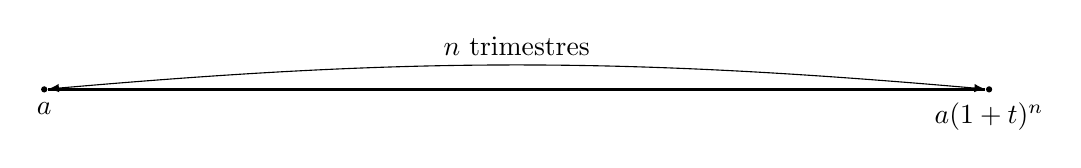
\begin{tikzpicture}
			\draw (0,0) node[circle, inner sep=0.8pt, fill=black, label={below:{$a$}}] (C) {};  
			\draw (12,0) node[circle, inner sep=0.8pt, fill=black, label={below:{$a(1+t)^n$}}] (D) {};  
			\draw[<->,>=latex] (C) to [bend left=5] node[above] {$n$ trimestres} (D); 
			\draw[line width=1.2pt] (C) to   (D); 
		\end{tikzpicture} \hspace{3cm}\null
		\vspace{-1em}
		\item  le 2\ieme versement de $a$ est placé $n-1$ trimestres, à taux d'initêret composés $t$ rapporte \dotfill $a(1+t)^{\ldots\ldots}$. \\
		\null\hfill 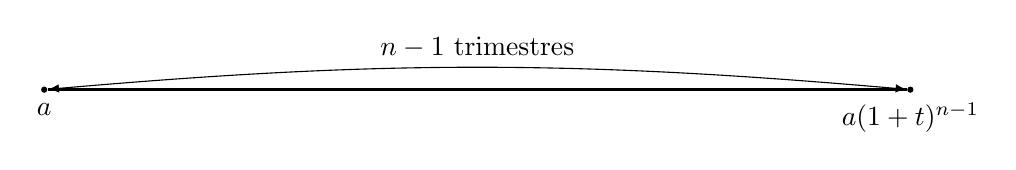
\begin{tikzpicture}
			\draw (0,0) node[circle, inner sep=0.8pt, fill=black, label={below:{$a$}}] (C) {};  
			\draw (11,0) node[circle, inner sep=0.8pt, fill=black, label={below:{$a(1+t)^{n-1}$}}] (D) {};  
			\draw[<->,>=latex] (C) to [bend left=5] node[above] {$n-1$ trimestres} (D); 
			\draw[line width=1.2pt] (C) to   (D); 
		\end{tikzpicture}\hspace{3cm} \null
		\vspace{-1em}
		\item  le 3\ieme versement de $a$ est placé $n-2$ trimestres, à taux d'initêret composés $t$ rapporte \dotfill $a(1+t)^{\ldots\ldots}$.\\
		\null\hfill 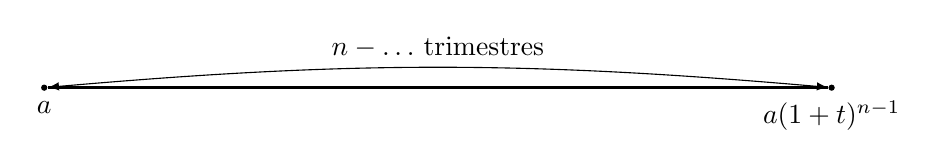
\begin{tikzpicture}
			\draw (0,0) node[circle, inner sep=0.8pt, fill=black, label={below:{$a$}}] (C) {};  
			\draw (10,0) node[circle, inner sep=0.8pt, fill=black, label={below:{$a(1+t)^{n-1}$}}] (D) {};  
			\draw[<->,>=latex] (C) to [bend left=5] node[above] {$n-\ldots$ trimestres} (D); 
			\draw[line width=1.2pt] (C) to   (D); 
		\end{tikzpicture} \hspace{3cm}\null
	\vspace{-1em}
		\item[$\ldots$] 
		\item le $n-1$\ieme versement de $a$ est placé $\ldots$ trimestres à taux d'initêret composés $t$ rapporte \dotfill $a(1+t)^{\ldots\ldots}$. \\
		\null\hfill 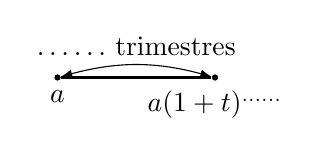
\begin{tikzpicture}
			\draw (0,0) node[circle, inner sep=0.8pt, fill=black, label={below:{$a$}}] (C) {};  
			\draw (2,0) node[circle, inner sep=0.8pt, fill=black, label={below:{$a(1+t)^{\ldots\ldots}$}}] (D) {};  
			\draw[<->,>=latex] (C) to [bend left=15] node[above] {$ \ldots\ldots$ trimestres} (D); 
			\draw[line width=1.2pt] (C) to   (D); 
		\end{tikzpicture} \hspace{3cm}\null
	\vspace{-1em}
		\item le $n$\ieme versement de $a$ est placé $\ldots$ trimestre à taux d'initêret composés $t$ rapporte \dotfill $a(1+t)^{\ldots\ldots}$.\\
		\null\hfill 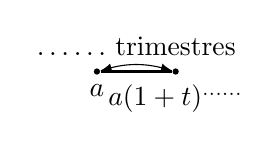
\begin{tikzpicture}
			\draw (0,0) node[circle, inner sep=0.8pt, fill=black, label={below:{$a$}}] (C) {};  
			\draw (1,0) node[circle, inner sep=0.8pt, fill=black, label={below:{$a(1+t)^{\ldots\ldots}$}}] (D) {};  
			\draw[<->,>=latex] (C) to [bend left=15] node[above] {$\ldots\ldots$ trimestres} (D); 
			\draw[line width=1.2pt] (C) to   (D); 
		\end{tikzpicture} \hspace{3cm}\null
	\vspace{-1em}
		\item à la fin du $n$\ieme trimestre le capital accumulé $C_n$ est :
		\item $		C_n=a(1+t)^{\ldots\ldots}+a(1+t)^{\ldots\ldots}+\ldots +a(1+t)^{\ldots\ldots}+a(1+t)^{\ldots\ldots}+a(1+t)^{n}$
		\item $C_n=$\dotfill 
	\end{enumerate}
\end{spacing}
\vspace{-0.75em} 
\end{problem}
\begin{exercise}\label{chapter05:exercise:suites48}\hfill \\
	On effectue 10 versements chaque début d'année de   \EUR{1000} sur un compte rapportant  8\% de taux d'intérêts composés par an (sans retraits possibles). Exprimer le capital accumulé à la fin de la 10\ieme année. 
\end{exercise}

\begin{problem}\label{chapter05:exercise:suites49}\hfill \\
On emprunte une somme $V_0 =$\EUR{500000} au taux d'intêret annuel de $5\%$. On souhaite rembourser cet emprunt en $10$ versement au début de chaque année.
\begin{enumerate}[leftmargin=*,label=\arabic*)]
	\item Détérminer le capital à rembourser après 10 ans en tenant compte des intêrets composés.
	\item Au terme de 10 années, l'imprunteur doit couvrir la somme précédente avec $10$ versements en début d'année de $a$, qui rapporteraient le taux d'intérêt annuel de $5\%$. En déduire que $a$ vérifie :
	\setlength{\abovedisplayskip}{3pt}
	\setlength{\belowdisplayskip}{3pt}
	\[
	500000\times 1.05^{10}=a\frac{1.05}{0.05}\left( 1.05^{10}-1 \right)
	\]
	\item Déduire $a$.
\end{enumerate} 
\end{problem}

\begin{exercise}\label{chapter05:exercise:suites50}\hfill 
\begin{enumerate}[leftmargin=*,label=\arabic*)]
	\item Montrer que pour tout $k\in\mathbb{N}$ : $(k+1)^3-k^3=3k^2+3k+1$
	\item Compléter : 
	\begin{spacing}{2}
		\vspace{-0.5em}
		\begin{enumerate}[leftmargin=*,label={}]
			\item  Si $k=1$ alors \dotfill $2^3-1^3=3\times 1^2+ 3\times 1 + 1$
			\item  Si $k=2$ alors \dotfill $3^3-2^3=3\times 2^2+ 3\times 2 + 1$
			\item  Si $k=3$ alors \dotfill $4^3-3^3=3\times 3^2+ 3\times 3 + 1$
			\item[...] 
			\item  Si $k=n$ alors \dotfill $(n+1)^3-n^3=3\times n^2+ 3\times n + 1$
			\item En ajoutant les égalités précédentes on obtient :
			\item $(n+1)^3-1^3= \ldots (1^2+2^2+3^2+\ldots +n^2)+\ldots(1+2+3+\ldots+n) + \ldots $
			\item $\ldots (1^2+2^2+3^2+\ldots +n^2)=(n+1)^3-\frac{\qquad\qquad\qquad }{2}-\dotfill $
		\end{enumerate}
	\end{spacing}
	\vspace{-0.75em}
	\item En déduire que $1^2+2^2+\ldots +n^2=\frac{n(n+1)(2n+1)}{6}$\medskip
	\item Déterminer $1^2+2^2+3^2+\ldots +10^2$ et $8^2+9^2+10^2+\ldots+15^2$.
\end{enumerate} 
\end{exercise}
\begin{problem}\label{chapter05:exercise:suites51} \hfill
	\begin{enumerate}[leftmargin=*,label=\arabic*)]
		\item Montrer que pour tout $k\in\mathbb{N}$ : $(k+1)^4-k^4=4k^3+6k^2+4k+1$
		\item En suivant la démarche de l'exercice précédent, montrer que $1^3+2^3+3^3+\ldots + n^3=\left(\frac{n(n+1)}{2}\right)^2$
		\item Utiliser l'identité pour retrouver $6^3+7^3+8^3+\ldots+13^3$.
	\end{enumerate} 
\end{problem}
\begin{problem} \label{chapter05:exercise:suites52} 
On considère les suites $u$, $v$ et $w$ définies par : 
\setlength{\abovedisplayskip}{3pt}
\setlength{\belowdisplayskip}{3pt}
$$
\begin{cases}
	u_0=0 \qquad u_1=1 \\
	\text{pour tout $n\in\mathbb{N}$} \quad  u_{n+2}=5u_{n+1}-6u_n
\end{cases}
\qquad 
	 \text{pour tout $n\in\mathbb{N}$} \quad  v_n=u_{n+1}-2u_n
	 \quad 
	 \text{et} \quad  w_n=u_{n}-3^{n}
$$ 
\begin{enumerate}[leftmargin=*,label=\arabic*)]
	\item Montrer que $v$ est une suite géométrique, et donner sa forme explicite.
	\item En déduire que pour tout $n\in\mathbb{N}$ : $u_{n+1}=2u_n+3^n$.
	\item Montrer que $w$ est une suite géométrique, et donner sa forme explicite.
	\item En déduire que pour tout $n\in\mathbb{N}$ on a $u_n=3^n-2^n$.
	\item Exprimer $S_n=\sum_{k=0}^{n} u_k$ en fonction de $n$. 
\end{enumerate} 
\end{problem}
\begin{exercise}
Soit une suite $(u_n)$ tel que pour tout $n\geqslant 1$, la somme des premiers $n$ termes d'une suite géométrique est égale à $5(3^n-1)$
\begin{enumerate}[leftmargin=*,label=\arabic*)]
	\item Quelle est la somme des $90$ premiers termes ?
	\item Montrer que pour tout $n\geqslant 1$ on a $u_n=k(3^n)$. Déterminer $k$.
\end{enumerate}
\end{exercise}
\begin{exercise} 
	\begin{enumerate}[leftmargin=*,label=\arabic*)]
		\item Déterminer $\sum_{r=3}^{10}3^r$.
		\item Montrer que $\sum_{r=1}^{15}(2^r-12r)=64094$.
	\end{enumerate}
\end{exercise}
\begin{exercise}\hfill 
\\
\noindent
\parbox{0.65\linewidth}{
Un élève a programme le dessin ci-contre formé d'une spirale formée de segments perpendiculaires. Le premier segment est de \SI{4}{\milli\meter} de long, et chaque segment est 25\% plus long que le précédent. 
\begin{enumerate}[leftmargin=*,label=\arabic*)]
	\item Détermine la longueur des 8 premiers segments tracés en \si{\milli\meter}.
	\item Détermine la longueur de la spirale en \si{\meter} formée de 20 segments.
\end{enumerate}
}
\hfill 
\parbox{0.3\linewidth}{\centering
\begin{tikzpicture}[yscale=1.25,xscale=1.25]
	\tkzSetUpPoint[size=3, fill=black]
	\tkzfctset{tan style/.style={->,>=latex, color=red, line width=1.2pt}}   
	\tkzSetUpLine[line width= 1.2pt, add=.5 and .5]  
	\tkzInit[xmin=-3,xmax=3,ymin=-3.0,ymax=3,xstep=1.0, ystep=1.0]; 
%	\begin{scope}[dashed]  
%		\tkzGrid[   color=gray](-5,-5)(5,5); 
%	\end{scope}
%	\tkzDrawX[above=5pt, label={$x$}, font=\small, line width=1.2pt] 
%	\tkzDrawY[right=5pt, label={$y$}, font=\small, line width=1.2pt] 
%	\tkzLabelX[  font=\scriptsize ]  
%	\tkzLabelY[orig=false,  font=\scriptsize]     
	
	\tikzmath{
		function f(\u) {%
			return 1.25*\u;
		};
		real \u0, \u1, \u2, \u3, \u4;
		\u0=0.40;
		\u1=f(\u0);
		\u2=f(\u1);
		\u3=f(\u2);
		\u4=f(\u3);
		\u5=f(\u4);
		\u6=f(\u5);
		\u7=f(\u6);
		\u8=f(\u7);
		\u9=f(\u8);
		\uv1=f(\u9);
		\uv2=f(\uv1);
	}
%	\newcount\j
%	\foreach \i in {0,1,2,3,4,5}{%
%		\pgfmathsetcount{\j}{\i+1}
%		\draw[dashed,line width=.2pt] (\u\i,0) node[below=8pt] {$u_\i$} -- (\u\i,{f(\u\i)}) ;%-- (0,{f(\u\i)}) node[left]	{$u_{\the\j}$};
%	}
	
	\draw[line width=2pt, red] (0,0) -- (0,\u0) -- (\u1,\u0)   -- (\u1,\u0-\u2) -- (\u1-\u3,\u0-\u2) --  (\u1-\u3,\u0-\u2+\u4) -- (\u1-\u3+\u5,\u0-\u2+\u4)   --(\u1-\u3+\u5,\u0-\u2+\u4-\u6) -- (\u1-\u3+\u5-\u7,\u0-\u2+\u4-\u6)  -- (\u1-\u3+\u5-\u7,\u0-\u2+\u4-\u6) -- (\u1-\u3+\u5-\u7,\u0-\u2+\u4-\u6+\u8) -- (\u1-\u3+\u5-\u7+\u9,\u0-\u2+\u4-\u6+\u8)  ;%-- (\u1-\u3+\u5-\u7+\u9,\u0-\u2+\u4-\u6+\u8-\uv1) -- (\u1-\u3+\u5-\u7+\u9-\uv2,\u0-\u2+\u4-\u6+\u8-\uv1)  ;
	 	
\end{tikzpicture} 
}
\end{exercise} 
\begin{exercise}\hfill 
	\\
	\noindent
\parbox{0.65\linewidth}{
	Un élève a programme le dessin ci-contre formé d'une spirale formée de segments perpendiculaires.  On note $u_n$ la longueur du $n-$\ieme segment.
	\begin{enumerate}[leftmargin=*,label=\arabic*)]
		\item Détermine la longueur des 8 premiers segments tracés en \si{\milli\meter}. 
		\item Donner une relation de récurrence vérifiée par la suite $(u_n)$.
		\item Détermine la longueur de la spirale en \si{\meter} formée de 20 segments.
	\end{enumerate}
}
\hfill 
\parbox{0.3\linewidth}{\centering
	\begin{tikzpicture}[yscale=0.5,xscale=0.5]
		\tkzSetUpPoint[size=3, fill=black]
		\tkzfctset{tan style/.style={->,>=latex, color=red, line width=1.2pt}}   
		\tkzSetUpLine[line width= 1.2pt, add=.5 and .5]  
		\tkzInit[xmin=-3,xmax=4,ymin=-3.0,ymax=4,xstep=1.0, ystep=1.0]; 
		\begin{scope}[dashed]  
				\tkzGrid[   color=gray](-3,-3)(4,4); 
			\end{scope}
		%	\tkzDrawX[above=5pt, label={$x$}, font=\small, line width=1.2pt] 
		%	\tkzDrawY[right=5pt, label={$y$}, font=\small, line width=1.2pt] 
		%	\tkzLabelX[  font=\scriptsize ]  
		%	\tkzLabelY[orig=false,  font=\scriptsize]     
		
		\tikzmath{
			function f(\u) {%
				return 1+\u;
			};
			real \u0, \u1, \u2, \u3, \u4;
			\u0=1;
			\u1=1;
			\u2=f(\u0);
			\u3=f(\u1);
			\u4=f(\u2);
			\u5=f(\u3);
			\u6=f(\u4);
			\u7=f(\u5);
			\u8=f(\u6);
			\u9=f(\u7);
			\uv1=f(\u8);
			\uv2=f(\u9);
		}
		%	\newcount\j
		%	\foreach \i in {0,1,2,3,4,5}{%
			%		\pgfmathsetcount{\j}{\i+1}
			%		\draw[dashed,line width=.2pt] (\u\i,0) node[below=8pt] {$u_\i$} -- (\u\i,{f(\u\i)}) ;%-- (0,{f(\u\i)}) node[left]	{$u_{\the\j}$};
			%	}
		
		\draw[line width=2pt, red] (0,0) -- (0,\u0) -- (\u1,\u0)   -- (\u1,\u0-\u2) -- (\u1-\u3,\u0-\u2) --  (\u1-\u3,\u0-\u2+\u4) -- (\u1-\u3+\u5,\u0-\u2+\u4)   --(\u1-\u3+\u5,\u0-\u2+\u4-\u6) -- (\u1-\u3+\u5-\u7,\u0-\u2+\u4-\u6)  -- (\u1-\u3+\u5-\u7,\u0-\u2+\u4-\u6) -- (\u1-\u3+\u5-\u7,\u0-\u2+\u4-\u6+\u8) -- (\u1-\u3+\u5-\u7+\u9,\u0-\u2+\u4-\u6+\u8)  ;%-- (\u1-\u3+\u5-\u7+\u9,\u0-\u2+\u4-\u6+\u8-\uv1) -- (\u1-\u3+\u5-\u7+\u9-\uv2,\u0-\u2+\u4-\u6+\u8-\uv1)  ;
		
	\end{tikzpicture} 
}
\end{exercise} 
%----------------------------------------------------------------------------------------
%	 
%----------------------------------------------------------------------------------------
\newpage 
\loadgeometry{widelayout}  
\pagestyle{scrheadings} % Print headers again  
\KOMAoptions{
	headwidth=textwithmarginpar,
	headsepline=true,
	headsepline= 0.5pt,
	footwidth=textwithmarginpar,
}  
\onehalfspacing  
\section{Exercices :corrections}
  
\begin{proof}[correction exercice \ref{chapter05:exercise:suites01}] \hfill 
	\begin{spacing}{2}
\begin{enumerate}[label=\alph*),leftmargin=*]
	\item $u_0=10$; $u_1=12$; $u_2=14$; $u_3=\colorbox{BurntOrange}{14} $ ; $u_4=\colorbox{BurntOrange}{16}$ ; $u_5=\colorbox{BurntOrange}{18}$ ; $u_6=\colorbox{BurntOrange}{20}$ \hfill \fbox{$u_{n+1}=u_n+2$}
	\item $u_0=-7$; $u_1=-2$; $u_2=3$; $u_3=\colorbox{BurntOrange}{8}$ ; $u_4=\colorbox{BurntOrange}{13}$  ; $u_5=\colorbox{BurntOrange}{18}$ ; $u_6=\colorbox{BurntOrange}{23}$\hfill \hfill \fbox{$u_{n+1}=u_n+5$} 
	\item $u_0=20$; $u_1=10$; $u_2=5$; $u_3=\colorbox{BurntOrange}{2.5}$ ; $u_4=\colorbox{BurntOrange}{1.25}$  ; $u_5=\colorbox{BurntOrange}{0.625}$ ; $u_6=\colorbox{BurntOrange}{0.3125}$\hfill \hfill \fbox{$u_{n+1}=\tfrac{1}{2} u_n$}
	\item $u_0=5$; $u_1=10$; $u_2=20$; $u_3=\colorbox{BurntOrange}{40}$ ; $u_4\colorbox{BurntOrange}{80}$  ; $u_5=\colorbox{BurntOrange}{160}$ ; $u_6=\colorbox{BurntOrange}{320}$\hfill \hfill  \fbox{$u_{n+1}=2 u_n$}
	\item $u_0=-12$; $u_1=\colorbox{BurntOrange}{-9}$; $u_2=\colorbox{BurntOrange}{-6}$; $u_3=\colorbox{BurntOrange}{-3}$ ; $u_4=\colorbox{BurntOrange}{0}$  ; $u_5=\colorbox{BurntOrange}{3}$   \hfill \hfill  \fbox{$u_{n+1}=u_n+3$}
	\item $u_0=6$; $u_1=\colorbox{BurntOrange}{-4}$; $u_2=\colorbox{BurntOrange}{-14}$; $u_3=\colorbox{BurntOrange}{-24}$ ; $u_4=\colorbox{BurntOrange}{-34}$  ; $u_5=\colorbox{BurntOrange}{-44}$   \hfill \hfill  \fbox{$u_{n+1}=u_n-10$}
	\item $u_0=1$; $u_1=\colorbox{BurntOrange}{9}$; $u_2=\colorbox{BurntOrange}{33}$; $u_3=\colorbox{BurntOrange}{105}$ ; $u_4=\colorbox{BurntOrange}{321}$  ; $u_5=\colorbox{BurntOrange}{969}$   \hfill \hfill  \fbox{$u_{n+1}=3(u_n+2)$}
	\item $u_0=5$; $u_1=\colorbox{BurntOrange}{-15}$; $u_2=\colorbox{BurntOrange}{25}$; $u_3=\colorbox{BurntOrange}{-55}$ ; $u_4=\colorbox{BurntOrange}{105}$  ; $u_5=\colorbox{BurntOrange}{-215}$   \hfill \hfill \fbox{$u_{n+1}=-2u_n-5$}
\end{enumerate} 
\end{spacing}\vspace{-0.5em}
\end{proof}
\begin{proof}[correction exercice \ref{chapter05:exercise:suites02}] \hfill 
\begin{spacing}{2}
\vspace{-1.0em}
\begin{description} 
	\item[arithmétique] $u_0=0.8$; $u_1=0.75$; $u_2=0.7$; $u_3=0.65$ ; $u_4=\ldots\ldots$  ;  \hfill  {$u_{n+1}=\colorbox{BurntOrange}{$u_n-0.05$} $} 
	\item[arithmétique] $u_0=-5$; $u_1=-7$; $u_2=-9$; $u_3=-11$ ; $u_4=\ldots\ldots$  ;  \hfill  {$u_{n+1}=\colorbox{BurntOrange}{$u_n-2$} $} 
	\item[arithmétique] $u_0=-2.6$; $u_1=-2.4$; $u_2=-2.2$; $u_3==\ldots\ldots$ ;    \hfill  {$u_{n+1}=\colorbox{BurntOrange}{$u_n+0.2$} $} 
	\item[arithmétique] $u_0=\tfrac{1}{4}$; $u_1=\tfrac{2}{4}$; $u_2=\tfrac{3}{4}$; $u_3=1$ ; $u_4=\ldots\ldots$  ;  \hfill  {$u_{n+1}=\colorbox{BurntOrange}{$u_n+\tfrac{1}{4}$} $} 
	\item[géométrique] $u_0=1$; $u_1=3$; $u_2=9$; $u_3= \ldots\ldots$  ;  \hfill  {$u_{n+1}=\colorbox{BurntOrange}{$3u_n$} $}
	\item[géométrique] $u_0=2$; $u_1=20$; $u_2=200$; $u_3= \ldots\ldots$  ;  \hfill  {$u_{n+1}=\colorbox{BurntOrange}{$10u_n$} $}
	\item[géométrique] $u_0=2$; $u_1=-10$; $u_2=50$; $u_3= \ldots\ldots$  ;  \hfill  {$u_{n+1}=\colorbox{BurntOrange}{$-5u_n$} $}
	\item[géométrique] $u_0=1$; $u_1=-1$; $u_2=1$; $u_3= \ldots\ldots$  ;  \hfill  {$u_{n+1}=\colorbox{BurntOrange}{$-u_n$} $}
	\item[Fibonacci] $u_0=1$; $u_1=1$; $u_2=2$; $u_3= \ldots\ldots$  ;  \hfill  {$\colorbox{BurntOrange}{$u_{n+1}=u_{n+1}+u_n$} $}
	\item[Fibonacci] $u_0=2$; $u_1=2$; $u_2=4$; $u_3= \ldots\ldots$  ;  \hfill  {$ \colorbox{BurntOrange}{$u_{n+1}=u_{n+1}+u_n$}  $}
\end{description} 
\end{spacing}\vspace{-0.5em}
\end{proof}
\begin{proof}[correction exercice \ref{chapter05:exercise:suites03}] \hfill
\vspace{-1em}
\begin{spacing}{2}
	\begin{description} 
		\item  $u_0=12$; $u_1=3$; $u_2=\colorbox{BurntOrange}{$-6$}$; $u_3=-15$ ;\hfill $u_{10}=\colorbox{BurntOrange}{$12-9\times 10=-78$}$  ;  \hfill  {$r=\colorbox{BurntOrange}{$-9$}  $}  
		\item  $u_0=4$; $u_1=\ldots\ldots$; $u_2=14$; $u_3=\colorbox{BurntOrange}{$9$}$ ; \hfill$u_{10}=\colorbox{BurntOrange}{$54$}$  ;  \hfill  {$r=\colorbox{BurntOrange}{$\frac{14-4}{2-0}=5$}  $}  
		\item  $u_0=7$; $u_1=\colorbox{BurntOrange}{$11$}$; $u_2=\colorbox{BurntOrange}{$15$}$; $u_3=19$ ; \hfill$u_{10}=\colorbox{BurntOrange}{$47$}$  ;  \hfill  {$r=\colorbox{BurntOrange}{$\frac{19-7}{3-0}=4$}  $}   
		\item  $u_0=1.3$; $u_1=\colorbox{BurntOrange}{$0.6$}$; $u_2=\colorbox{BurntOrange}{$-0.1$}$; $u_3=-0.8$ ; \hfill$u_{10}=\colorbox{BurntOrange}{$-5.7$}$  ;  \hfill  {$r=\colorbox{BurntOrange}{$\frac{u_3-u_0}{3-0}=-0.7$}$}  
	\end{description} 
\end{spacing}\vspace{-1em}
\end{proof}
%
\begin{proof}[correction exercice \ref{chapter05:exercise:suites04}] \hfill 
\vspace{-1em}
\begin{spacing}{2}
	\begin{description} 
		\item  $u_0=3$; $u_1=12$; $u_2=\colorbox{BurntOrange}{$48$}$; $u_3=\colorbox{BurntOrange}{$192$}$ ;\hfill $u_{10}=\colorbox{BurntOrange}{$3\times 4^{10}$}$  ;  \hfill  {$q=\colorbox{BurntOrange}{$\frac{u_1}{u_0}=4$}  $}  
		\item  $u_0=12$; $u_1=\colorbox{BurntOrange}{$24$}$; $u_2=48$; $u_3=\colorbox{BurntOrange}{$96$}$ ; \hfill$u_{10}=\colorbox{BurntOrange}{$12\times 2^{10}$}$    \hfill  {$q=\colorbox{BurntOrange}{$\sqrt{\frac{u_2}{u_0}}=\sqrt{\frac{48}{12}}=2$}  $}  
		\item  $u_0=4$; $u_1=\colorbox{BurntOrange}{$12$}$; $u_2=\colorbox{BurntOrange}{$36$}$; $u_3=108$ ; \hfill$u_{10}=\colorbox{BurntOrange}{$4\times 3^{10}$}$    \hfill  {$q=\colorbox{BurntOrange}{$\sqrt[3]{\frac{u_3}{u_0}}=\sqrt[3]{\frac{108}{4}}=3$}$}   
		\item  $u_0=6$; $u_1=\colorbox{BurntOrange}{$60$}$; $u_2=\colorbox{BurntOrange}{$600$}$; $u_3=6000$ ; \hfill$u_{10}=\colorbox{BurntOrange}{$6\times 10^{10}$}$     \hfill  {$q=\colorbox{BurntOrange}{$\sqrt[3]{\frac{u_3}{u_0}}=\sqrt[3]{\frac{6000}{6}}=10$}  $}  
	\end{description} 
\end{spacing}\vspace{-1em}
\end{proof}
\begin{proof}[correction exercice \ref{chapter05:exercise:suites05}] \hfill 
	
\newlength\radiusc
\pgfmathsetlength{\radius}{0.2cm}
\newcommand\drawballs[2][]{%
	\foreach \y [evaluate=\y as \yy using #2+1-\y] in {1,...,#2} {%
		\foreach \x in {1,...,\yy} {%
			\shade[shading=ball,ball color=white,#1] 
			({(2*\x-2+\y)*\radius},{sqrt(3)*\y*\radiusc}) circle (\radiusc); 
		};
	}%
}  	
\noindent\hfill 
\begin{tikzpicture}
	\drawballs{1}
	\drawballs[xshift=2cm]{2}
	\drawballs[xshift=4cm]{3}
	\drawballs[xshift=7cm]{4}
	\drawballs[xshift=10cm]{5}
	\tkzText[](0,-0.5){$u_1=1$}
	\tkzText[](2.5,-0.5){$u_2=u_1+2$}
	\tkzText[](5,-0.5){$u_3=u_2+3$}
	\tkzText[](7.5,-0.5){$u_4=u_3+4$}
	\tkzText[](11,-0.5){$u_5=u_4+5$}
\end{tikzpicture}
\hfill \null
\begin{enumerate}[label=\arabic*),leftmargin=*]
	\item  les relations récurrences :\hfill $u_{n+1}=u_n+\colorbox{BurntOrange}{$n+1$}$ \hfill $u_{n}=\colorbox{BurntOrange}{$u_{n-1}$}+\colorbox{BurntOrange}{$u_n$}$
	\item  les 10 premiers nombres triangulaires sont  \colorbox{BurntOrange}{$0;~ 1;~ 3;~ 6;~ 10;~ 15;~ 21;~ 28;~ 36;~ 45;~ 55;~ 66;~ 78;~ 91;~ 105$}
\end{enumerate}	
\end{proof}
\begin{proof}[correction exercice \ref{chapter05:exercise:suites06}] \hfill 
	
\noindent
\begin{minipage}{0.62\linewidth} 
\begin{enumerate}[label=\arabic*),leftmargin=*]
	\item   les 4 premiers terme de la suite $(u)$ :\\
	$u_1=\colorbox{BurntOrange}{$\frac{1}{4}$}$\dotfill $u_2=\colorbox{BurntOrange}{$\frac{1}{8}$}$\dotfill $u_3=\colorbox{BurntOrange}{$\frac{1}{16}$}$\dotfill $u_4=\colorbox{BurntOrange}{$\frac{1}{32}$}$\dotfill 
	\item  relation de récurrence : \colorbox{BurntOrange}{$u_{n+1}=\frac{1}{4}u_n$} 
	\item Complétez le script Python pour calculer 
	\setlength{\abovedisplayskip}{3pt}
	\setlength{\belowdisplayskip}{3pt}
$$u_1+u_2+u_3+\ldots+u_{10}=$$	
\begin{lstlisting}[ language=python , 
%	title=Script B,   
linewidth=0.95\columnwidth,
style=python-code,    
aboveskip=0.0\topskip,
belowskip=0.0\topskip,
xleftmargin=1.2em,
%	lineskip=1.0em,
tabsize=4, 
%numbers=none,
%	firstnumber=10  
] 
def calcul() :
	nbr , u = 0  , 0.25
	for i in range(11) :
		nbr = nbr + u
		u = u/4
	return nbr
\end{lstlisting}
	\item  
	$u_1+u_2+u_3+\ldots +u_{100}\approx \colorbox{BurntOrange}{$\frac{1}{3}$} $
\end{enumerate}	 
\end{minipage} 
\hfill 
\begin{minipage}{0.35\linewidth} 
\begin{tikzpicture}[xscale=1.5, yscale=1.5]
	\tkzInit[xmin=-2.0,xmax=2.0,ymin=-1.0,ymax=3.0,xstep=1.0, ystep=1.0];
	\tkzSetUpPoint[size=4, fill=black]
	\tkzfctset{tan style/.style={->,>=latex, color=red, line width=1.2pt}}  
	
	\tkzDefPoint(0,0){A}
	\tkzDefPoint(2,0){B}
	\tkzDefPoint(4,0){B0}
	\tkzDefPoint(2,2){C}
	\tkzDefPoint(3,2){D}
	\tkzDefPoint(3,3){A1}
	\tkzDefPoint(3.5,3){B1}
	\tkzDefPoint(3.5,3.5){A2}
	\tkzDefPoint(3.75,3.5){B2}
	\tkzDefPoint(3.75,3.75){A3}
	\tkzDefPoint(3.875,3.75){B3}
	\tkzDefPoint(3.875,3.875){A4}
	\tkzDefPoint(3.9375,3.875){B4}
	
	\tkzDefSquare(A,B)\tkzGetPoints{E}{F}
	\tkzDefSquare(A,B0)\tkzGetPoints{E0}{F0}
	\tkzDefSquare(A1,B1)\tkzGetPoints{E1}{F1}
	\tkzDefSquare(A2,B2)\tkzGetPoints{E2}{F2}
	\tkzDefSquare(A3,B3)\tkzGetPoints{E3}{F3}
	\tkzDefSquare(A4,B4)\tkzGetPoints{E4}{F4} 
	\tkzDefSquare(C,D)\tkzGetPoints{G}{H}
	\tkzFillPolygon[draw,fill = gray!30 , line width=1.2pt](A,B,E,F)
	\tkzDrawPolygon[draw, line width=1.2pt ](A,B0,E0,F0)
	\tkzFillPolygon[draw,fill = gray!30, line width=1.2pt](C,D,G,H)
	\tkzFillPolygon[draw,fill = gray!30, line width=1.2pt ](A1,B1,E1,F1)
	\tkzFillPolygon[draw,fill = gray!30, line width=1.2pt ](A2,B2,E2,F2) 
	\tkzFillPolygon[draw,fill = gray!30 ](A3,B3,E3,F3) 
	\tkzFillPolygon[draw,fill = gray!30 ](A4,B4,E4,F4) 
	\tkzLabelSegment[](A,E){$u_1$}
	\tkzLabelSegment[](D,H){$u_2$}
	\tkzLabelSegment[above](A1,B1){$u_3$}
	\tkzLabelSegment[above,font=\scriptsize](A2,B2){$u_4$}
	\tkzDefPoint(4,2){I1}
	\tkzDefPoint(2,4){J1}
	\tkzDrawSegments(I1,D J1,H)
	
	\tkzDefPoint(4,3){I2}
	\tkzDefPoint(3,4){J2}
	\tkzDrawSegments(I2,B1 J2,F1)
	
	\tkzDefPoint(4,3.5){I3}
	\tkzDefPoint(3.5,4){J3}
	\tkzDrawSegments(I3,B2 J3,F2)
	
	\tkzDefPoint(4,3.75){I4}
	\tkzDefPoint(3.75,4){J4}
	\tkzDrawSegments(I4,E2 J4,E2)
	
	\tkzDefPoint(4,3.875){I5}
	\tkzDefPoint(3.875,4){J5}
	\tkzDrawSegments(I5,E3 J5,E3)
	
	\tkzDefPoint(4,3.9375){I6}
	\tkzDefPoint(3.9375,4){J6}
	\tkzDrawSegments(I6,E4 J6,E4)
	
	\tkzLabelSegment[below](A,B){\scriptsize$\frac{1}{2}$}
	\tkzLabelSegment[left](A,F){\scriptsize$\frac{1}{2}$}
	
	\tkzLabelSegment[below](C,D){\scriptsize$\frac{1}{4}$}
%	\tkzLabelSegment[below](A1,B1){\scriptsize$\frac{1}{8}$}
%	\tkzLabelSegment[below](A2,B2){\scriptsize$\tfrac{1}{16}$}
	\tkzLabelSegment[left](C,H){\scriptsize$\frac{1}{4}$}
%	\tkzLabelSegment[left](A1,F1){\scriptsize$\frac{1}{8}$}
%	\tkzLabelSegment[left](A2,F2){\scriptsize$\tfrac{1}{16}$}
\end{tikzpicture} 
\end{minipage}
\end{proof}
\begin{proof}[correction exercice \ref{chapter05:exercise:suites08}] \hfill Le grand rectangle est d'aire $1$. On note $u_n$ les aires de la suite des rectangles grisés. 
	
\noindent
\begin{minipage}{0.62\linewidth} 

\begin{enumerate}[label=\arabic*),leftmargin=*]
	 \item les 4 premiers terme de la suite $(u)$ :\\
	$u_1=\colorbox{BurntOrange}{$\frac{1}{3}$}$\dotfill $u_2=\colorbox{BurntOrange}{$\frac{1}{9}$}$\dotfill $u_3=\colorbox{BurntOrange}{$\frac{1}{27}$}$\dotfill $u_4=\colorbox{BurntOrange}{$\frac{1}{81}$}$\dotfill 
	\item  relation de récurrence : \colorbox{BurntOrange}{$u_{n+1}=\frac{1}{3}u_n$} 
	\item Complétez le script Python pour calculer $u_1+u_2+\ldots+u_n$ 
\begin{lstlisting}[ language=python , 
	%	title=Script B,   
	linewidth=0.95\columnwidth,
	style=python-code,    
	aboveskip=0.0\topskip,
	belowskip=0.0\topskip,
	xleftmargin=1.2em,
	%	lineskip=1.0em,
	tabsize=4, 
	%numbers=none,
	%	firstnumber=10  
	] 
def calcul(n) :
	nbr , u =  0  , 1/3
	for i in range( n  ) :
		nbr = nbr + u
		u = u/3
	return nbr
\end{lstlisting}
	\item  $u_1+u_2+u_3+\ldots +u_{100}\approx \colorbox{BurntOrange}{$\frac{1}{2}$}$
\end{enumerate}	 
\end{minipage} 
\hfill 
\begin{minipage}{0.35\linewidth} \centering
\begin{tikzpicture}[xscale=1.5, yscale=1.5]
\tkzInit[xmin=-2.0,xmax=2.0,ymin=-1.0,ymax=3.0,xstep=1.0, ystep=1.0];
\tkzSetUpPoint[size=4, fill=black]
\tkzfctset{tan style/.style={->,>=latex, color=red, line width=1.2pt}}  

\tkzDefPoint(0,0){A}
\tkzDefPoint(3,0){B}
\tkzDefPoint(3,4){C}
\tkzDefPoint(0,4){D}
\tkzDrawPolygon[draw, line width=1.2pt ](A,B,C,D)
\tkzDefBarycentricPoint(A=2,D=1)\tkzGetPoint{A0}
\tkzDefBarycentricPoint(A=1,D=2)\tkzGetPoint{A1}
\tkzDefBarycentricPoint(B=2,C=1)\tkzGetPoint{B0}
\tkzDefBarycentricPoint(B=1,C=2)\tkzGetPoint{B1}
\tkzDrawSegment[line width=1.2pt](A0,B0)
\tkzDrawPolygon[draw,fill = gray!30, line width=1.2pt ](A1,B1,C,D) 
\tkzLabelSegment[](A1,C){$u_1$}
\tkzDefBarycentricPoint(A0=2,B0=1)\tkzGetPoint{A00}
\tkzDefBarycentricPoint(A0=1,B0=2)\tkzGetPoint{A01}
\tkzDefBarycentricPoint(A1=2,B1=1)\tkzGetPoint{B00}
\tkzDefBarycentricPoint(A1=1,B1=2)\tkzGetPoint{B01}
\tkzDrawSegment[line width=1.2pt](A00,B00)
\tkzDrawPolygon[draw,fill = gray!30, line width=1.2pt ](A01,B01,B1,B0) 
\tkzLabelSegment[](A01,B1){$u_2$}
%
\tkzDefBarycentricPoint(A00=2,B00=1)\tkzGetPoint{A000}
\tkzDefBarycentricPoint(A00=1,B00=2)\tkzGetPoint{A001}
\tkzDefBarycentricPoint(A01=2,B01=1)\tkzGetPoint{B000}
\tkzDefBarycentricPoint(A01=1,B01=2)\tkzGetPoint{B001}
\tkzDrawSegment[line width=1.2pt](A000,B000)
\tkzDrawSegment[line width=1.2pt](A001,B001)
\tkzDrawPolygon[draw,fill = gray!30, line width=1.2pt ](B000,A000,A00,A01) 
\tkzLabelSegment[below](A000,B000){$u_3$}
%
\tkzDefBarycentricPoint(A000=2,B000=1)\tkzGetPoint{A0000}
\tkzDefBarycentricPoint(A000=1,B000=2)\tkzGetPoint{A0001}
\tkzDefBarycentricPoint(A001=2,B001=1)\tkzGetPoint{B0000}
\tkzDefBarycentricPoint(A001=1,B001=2)\tkzGetPoint{B0001}
\tkzDrawSegment[line width=1.2pt](A0000,B0000)
\tkzDrawSegment[line width=1.2pt](A0001,B0001)
\tkzDrawPolygon[draw,fill = gray!30, line width=1.2pt ](B0000,A0000,A000,A001) 
\tkzLabelSegment[left, font=\scriptsize](A0000,B0000){$u_4$} 
%
\tkzDefBarycentricPoint(A0000=2,B0000=1)\tkzGetPoint{A00000}
\tkzDefBarycentricPoint(A0000=1,B0000=2)\tkzGetPoint{A00001}
\tkzDefBarycentricPoint(A0001=2,B0001=1)\tkzGetPoint{B00000}
\tkzDefBarycentricPoint(A0001=1,B0001=2)\tkzGetPoint{B00001}
\tkzDrawSegment[line width=1.2pt](A00000,B00000)
\tkzDrawSegment[line width=1.2pt](A00001,B00001)
\tkzDrawPolygon[draw,fill = gray!30, line width=1.2pt ](B00001,A00001,B0000,B0001) 
%
\tkzDefBarycentricPoint(A00000=2,B00000=1)\tkzGetPoint{A000000}
\tkzDefBarycentricPoint(A00000=1,B00000=2)\tkzGetPoint{A000001}
\tkzDefBarycentricPoint(A00001=2,B00001=1)\tkzGetPoint{B000000}
\tkzDefBarycentricPoint(A00001=1,B00001=2)\tkzGetPoint{B000001}
\tkzDrawSegment[line width=1.2pt](A000000,B000000)
\tkzDrawSegment[line width=1.2pt](A000001,B000001)
\tkzDrawPolygon[draw,fill = gray!30, line width=1.2pt ](B000001,A000001,B00000,B00001) 
\end{tikzpicture} 
\end{minipage}
\end{proof}  
\begin{proof}[correction exercice \ref{chapter05:exercise:suites09}]   Dans chaque cas $u_n$ désigne le montant d'un placement après $n$ échéances. 
\begin{spacing}{2}
	\begin{description}
		\item[]\hfill\hfill \textbf{Relation de récurrence}\hfill \textbf{Forme explicite}
		\item[intérêts composés 5\%] $u_0=2000€$\hfill $u_{n+1}=\colorbox{BurntOrange}{$1.05$} u_n$\hfill $u_n=\colorbox{BurntOrange}{$2000\times 1.05^n$} $
		\item[intérêts composés 2\%] $u_0=4000€$\hfill $u_{n+1}=\colorbox{BurntOrange}{$1.02$} u_n$\hfill $u_n=\colorbox{BurntOrange}{$4000\times 1.02^n$} $
		\item[intérêts composés 1\%] $u_0=10000€$\hfill $u_{n+1}=\colorbox{BurntOrange}{$1.01$} u_n$\hfill $u_n=\colorbox{BurntOrange}{$10000\times 1.01^n$} $
		\item[intérêts simples 6\%] $u_0=100€$\hfill $u_{n+1}=\colorbox{BurntOrange}{$u_n+6$} \ldots\ldots$\hfill   $u_n=\colorbox{BurntOrange}{$100+ 6\times n$} $ 
		\item[intérêts simples 2\%] $u_0=3500€$\hfill $u_{n+1}=\colorbox{BurntOrange}{$u_n+70$} $\hfill   $u_n=\colorbox{BurntOrange}{$3500+ 70\times n$} $ 
		\item[dépréciation composée de 7\%] $u_0=500€$\hfill $u_{n+1}=\colorbox{BurntOrange}{$0.93u_n$}  $\hfill   $u_n=\colorbox{BurntOrange}{$500\times 0.93^n$} $ 
		\item[dépréciation composée de 12\%] $u_0=100€$\hfill $u_{n+1}=\colorbox{BurntOrange}{$0.88u_n$}$\hfill   $u_n=\colorbox{BurntOrange}{$100\times 0.88^n$} $ 
		\item[dépréciation composée de 9\%] $u_0=300€$\hfill $u_{n+1}=\colorbox{BurntOrange}{$0.91u_n$}$\hfill   $u_n=\colorbox{BurntOrange}{$300\times 0.91^n$} $ 
		\item[intérêts composés 10\%] $u_1=400€$\hfill $u_{n+1}=\colorbox{BurntOrange}{$1.10u_n$} $\hfill $u_n=\colorbox{BurntOrange}{$400\times 1.10^{n-1}$} $
		\item[intérêts composés 4\%] $u_3=200€$\hfill $u_{n+1}=\colorbox{BurntOrange}{$1.04$}u_n$\hfill $u_n=\colorbox{BurntOrange}{$200\times 1.04^{n-3}$} $
		\item[intérêts composés 3\%] $u_5=100€$\hfill $u_{n+1}=\colorbox{BurntOrange}{$1.03$} u_n$\hfill $u_n=\colorbox{BurntOrange}{$100\times 1.03^{n-5}$} $
		\item[dépréciation composés de 3\%] $u_{2}=200€$\hfill $u_{n+1}=\colorbox{BurntOrange}{$0.97$} u_n$\hfill $u_n=\colorbox{BurntOrange}{$200\times 0.97^{n-2}$} $
		\item[dépréciation composés de 3\%] $u_{10}=300€$\hfill $u_{n+1}=\colorbox{BurntOrange}{$0.97$} u_n$\hfill $u_n=\colorbox{BurntOrange}{$300\times 0.97^{n-10}$} $
	\end{description}
\vspace{-1em}
\end{spacing} 
\end{proof} 
\begin{proof}[correction exercice \ref{chapter05:exercise:suites10}] \hfill  

\noindent\QCM[  VF, Stretch=1.3, NomV=arithmétique,NomF=non arithmétique, Largeur=3.5cm,Reponses=2,Solution,  ]%
{% 
{$u$ définie pour tout $n\in\mathbb{N}$ par $u_n=3n-2$}&1,%  
{$u$ définie par $u_0=3$ et pour tout $n\in\mathbb{N}$  on  $u_{n+1}= u_{n}-\tfrac{1}{3}$}&1,%    
{$u$ définie pour tout $n\in\mathbb{N}$ par $u_n=5n-2$}&1,%  
{$u$ définie par $u_0=5$ et pour tout $n\in\mathbb{N}$   $u_{n+1}=2u_{n}+5$}&2,% 
{$u$ définie pour tout $n\in\mathbb{N}$ par $u_n=n^2-n$}&2,% 
{$u$ définie pour tout $n\in\mathbb{N}$ par $u_n=2n-5$}&1,%  
{$u$ définie pour tout $n\in\mathbb{N}$ par $u_n=-n+3$}&1,%      
{$u$ définie par $u_0=-2$ et pour tout $n\in\mathbb{N}$ on a  $u_{n+1}=u_{n}+5$}&1%
} 
\end{proof} 
%
\begin{proof}[correction exercice \ref{chapter05:exercise:suites11}] \hfill   
	
\noindent\QCM[  VF, Stretch=1.3, NomV=géométrique,NomF=non géométrique, Largeur=3.5cm,Reponses=2,Solution,  ]%
{  
	{$u$ définie pour tout $n\in\mathbb{N}$ par $u_n=4^n$}&1,%   
	{$u$ définie pour tout $n\in\mathbb{N}$ par $u_n=7\times 0.5^n$}&1,%   
	{$u$ définie par $u_0=5$ et pour tout $n$, $u_{n+1}=\numprint{1.05}u_{n}$}&1,%
{$u$ définie par $u_0=3$ et pour tout $n\in\mathbb{N}$,  $u_{n+1}=\frac{u_{n}}{2}$}&1,% 
{$u$ définie pour tout $n$, $u_{n+1}=\numprint{1.1}n$}&2,% 
{$u$ définie  pour tout $n$, $u_{n+1}=n^4$}&2,%
	  {$u$ définie par $u_0=5$ et pour tout $n$, $u_{n+1}=5u_{n}+1$}&2,%
	{$u$ définie pour tout $n\in\mathbb{N}$ par $u_n=3^{-n}$}&1,%   
} 


\end{proof} 
\begin{proof}[correction exercice \ref{chapter05:exercise:suites12}]      Les suites $u$ sont \textbf{arithmétiques} de raison $r$.  
% \vspace{-0.5em}
%\begin{multicols}{4}
\begin{enumerate}[label=\arabic*),leftmargin=*]
	\item $u_0=-3$ et $r=-\tfrac{1}{2}$. \colorbox{BurntOrange}{$u_n=-3-\frac{1}{2}\times n$; $u_{100}=-53$}
	\item $u_1=5$ et $r=\tfrac{1}{10}$. \colorbox{BurntOrange}{$u_n=5+\frac{1}{10}\times (n-1)$; $u_{100}=14.9$}
	\item $u_5=-\tfrac{1}{3}$ et $r=\tfrac{1}{2}$. \colorbox{BurntOrange}{$u_n=-\frac{1}{3}+\frac{1}{2}\times (n-5)$; $u_{100}=\frac{283}{6}$}
	\item $u_{10}=0$ et $r=-\tfrac{1}{3}$.  \colorbox{BurntOrange}{$u_n=0-\frac{1}{3}\times (n-10)$; $u_{100}=-30$}
\end{enumerate}
%\end{multicols}
\end{proof}
\vspace{-0.5em} 
\begin{proof}[correction exercice \ref{chapter05:exercise:suites13}]   suites \textbf{arithmétique} suivantes déterminer la raison $r$ et déduire la forme explicite.
%\vspace{-0.5em}
%\begin{multicols}{3}
	\begin{enumerate}[label=\arabic*),leftmargin=*]
		\item $u_0=3$ et $u_{1}=7$.   \colorbox{BurntOrange}{$r=u_{1}-u_{0}=4$ et $u_n=4n+3$}
		\item $u_0=3$ et $u_{2}=7$.   \colorbox{BurntOrange}{$r=\frac{u_{2}-u_{0}}{2-0}=2$ et $u_n=2n+3$}
		\item $u_1=-4$ et $u_{10}=38$.  \colorbox{BurntOrange}{$r=\frac{u_{10}-u_{1}}{10-1}=\frac{14}{3}$ et $u_n=\frac{14}{3}(n-1)-4$}
		\item $u_1=5$ et $u_{100}=-45$. \colorbox{BurntOrange}{$r=\frac{u_{100}-u_{1}}{100-1}=\frac{-50}{99}$ et $u_n=\frac{-50}{99}(n-1)+5$}
		\item $u_2=4$ et $u_8=-6$.  \colorbox{BurntOrange}{$r=\frac{u_{8}-u_{2}}{8-2}=\frac{-5}{3}$ et $u_n=\frac{-5}{3}(n-2)+4$}
		\item $u_5=27$ et $u_{10}=33$.  \colorbox{BurntOrange}{$r=\frac{u_{10}-u_{5}}{10-5}=\frac{6}{5}$ et $u_n=\frac{6}{5}(n-5)+27$} 
%		\item $u_{20}=3$ et $u_{15}=10$. 
%		\item $u_4=\tfrac{1}{6}$ et $u_{6}=\tfrac{1}{4}$. 
	\end{enumerate}
%\end{multicols}
\end{proof}
\vspace{-0.5em}
\begin{proof}[correction exercice \ref{chapter05:exercise:suites14}]        Les suites $u$ sont \textbf{géométriques} de raison $q$. \\
	Donner les formes explicites des suites arithmétiques suivantes et calculer $u_{10}$.
	\vspace{-0.5em}
%	\begin{multicols}{4}
		\begin{enumerate}[label=\arabic*),leftmargin=*]
			\item $u_0=4$ et $q=5$.   \colorbox{BurntOrange}{$u_n=4\times 5^{n}$; $u_{10}=4\times 5^{10}$}
			\item $u_0=\frac{1}{3}$ et $q=-2$.  \colorbox{BurntOrange}{$u_n=\frac{1}{3}\times (-2)^{n}$; $u_{10}=\frac{1}{3}\times (-2)^{10}$}
			\item $u_5=\num{3}$, et $q=\frac{1}{2}$.  \colorbox{BurntOrange}{$u_n=3\times \left(\frac{1}{2}\right)^{n-5}=3\times 2^{5-n}$; $u_{10}=3\times 2^{-5}$}
			\item $u_{20}=\num{10}$, et $q=\frac{-1}{3}$.  \colorbox{BurntOrange}{$u_n=10\times \left(\frac{-1}{3}\right)^{n-20}$; $u_{10}=10\times \left(\frac{-1}{3}\right)^{-10}=10\times (-3)^{10}$}
		\end{enumerate}
%	\end{multicols}
\end{proof}
\vspace{-0.5em}
\begin{proof}[correction exercice \ref{chapter05:exercise:suites15}] \hfill  
Pour les suites \textbf{géométriques} suivantes déterminer la raison $q$ et déduire la forme explicite.
\vspace{-0.5em}
%	\begin{multicols}{2}
		\begin{enumerate}[label=\arabic*),leftmargin=*]
			\item $u_0=\num{6}$, et $u_1=9$.  \colorbox{BurntOrange}{$q=\frac{u_1}{u_0}=\frac{9}{6}=\frac{3}{2}$; $u_{n}=6\times \left(\frac{3}{2}\right)^{n}$}
			\item $u_0=\num{1}$, et $u_2=9$. $q>0$. \colorbox{BurntOrange}{$q=\sqrt{\frac{u_2}{u_0}}=3$; $u_{n}=1\times 3^{n}$}
			\item $u_5=\num{486}$, et $u_7=4374$. $q>0$. \colorbox{BurntOrange}{$q=\sqrt{\frac{u_7}{u_5}}=3$; $u_{n}=486\times 3^{n-5}$}
			\item $u_2=\num{-1.92}$, et $u_4=\num{-1.2288}$. $q>0$. \colorbox{BurntOrange}{$q=\sqrt{\frac{u_4}{u_2}}=0.8$; $u_{n}=-1.92\times 0.8^{n-2}$}
			\item $u_5=100$ et $u_8=\numprint{6.25}$. $q<0$. \colorbox{BurntOrange}{$q=-\sqrt[3]{\frac{u_9}{u_5}}=0.5$; $u_{n}=1000\times (-0.5)^{n-5}$}
			\item $u_3=9$ et $u_7=2304$. $q<0$. \colorbox{BurntOrange}{$q=-\sqrt[4]{\frac{u_7}{u_3}}=-4$; $u_{n}=9\times (-4)^{n-3}$}
		\end{enumerate}
%	\end{multicols}
\end{proof} 
% 
%%----------------------------------------------------------------------------------------
%%	 
%%----------------------------------------------------------------------------------------
%\newpage 
\begin{proof}[correction exercice \ref{chapter05:exercise:suites16}] \hfill   Indiquer le sens de variation des suites suivantes.
	
 

\noindent\QCM[Multiple,Alterne,Solution, Stretch=1.3,  Largeur=2.2cm,Reponses=3,
Noms={croissante/décroissante/non monotone}]
{ 
	{$u$ définie pour tout $n\in\mathbb{N}$ par $u_n=3n-2$}&1&0&0,%  
	{$u$ définie par $u_0=3$ et pour tout $n\in\mathbb{N}$, $u_{n+1}=u_{n}+1$}&1&0&0,%   
	{$u$ définie par $u_0=5$ et pour tout $n\in\mathbb{N}$,  $u_{n+1}=2u_{n}$}&1&0&0,%   
	{$u$ définie par $u_0=-3$ et pour tout $n\in\mathbb{N}$,  $u_{n+1}=3u_{n}$}&0&1&0,%   
	{$u$ définie par $u_0=-1$ et pour tout $n\in\mathbb{N}$,  $u_{n+1}=0.5u_{n}$}&1&0&0,%
	{$u$ définie pour tout $n\in\mathbb{N}$ par $u_n=0.95^n$}&0&1&0,%  
	{$u$ définie pour tout $n\in\mathbb{N}$ par $u_n=1.10^n$}&1&0&0,% 
	{$u$ définie pour tout $n\in\mathbb{N}$ par $u_n=2^n+1$}&1&0&0,% 
	{$u$ définie pour tout $n\in\mathbb{N}$ par $u_n=-3^n+1$}&0&1&0,%  
	{$u$ définie pour tout $n\in\mathbb{N}$ par $u_n=1.05^n+3$}&1&0&0,% 
	{$u$ définie pour tout $n\in\mathbb{N}$ par $u_n=5+0.3^n$}&0&1&0,%  
	{$u$ définie pour tout $n\in\mathbb{N}$ par $u_n=3-0.25^n$}&0&1&0,% 
	{$u$ définie pour tout $n\in\mathbb{N}$ par $u_n=3+(-0.80)^n$}&0&0&1,%           
} 
\end{proof} 
 
\begin{proof}[correction exercice \ref{chapter05:exercise:suites17}] \hfill   Donner les limites lorsque $n\to\infty$ des suites suivantes.
\begin{spacing}{2}
\begin{enumerate}[label=\arabic*),leftmargin=*]
	\item $u$ définie pour tout $n\in\mathbb{N}$ par $u_n=5n^2-3n+2$. $\lim_{n\to\infty}u_n=$\colorbox{BurntOrange}{$+\infty$; diverge} 
	\item $u$ définie pour tout $n\in\mathbb{N}$ par $u_n=-n^2+2$. $\lim_{n\to\infty}u_n=$\colorbox{BurntOrange}{$-\infty$; diverge}  
	\item $u$ définie pour tout $n\in\mathbb{N}$ par $u_n=\frac{2n}{3n+1}$. $\lim_{n\to\infty}u_n=$\colorbox{BurntOrange}{$\frac{2}{3}$; converge} 
	\item $u$ définie pour tout $n\in\mathbb{N}$ par $u_n=2^n$. $\lim_{n\to\infty}u_n=$\colorbox{BurntOrange}{$+\infty$; diverge}  
	\item $u$ définie pour tout $n\in\mathbb{N}$ par $u_n=-1.5^n$. $\lim_{n\to\infty}u_n=$\colorbox{BurntOrange}{$-\infty$; diverge}  
	\item $u$ définie pour tout $n\in\mathbb{N}$ par $u_n=-0.5^n$. $\lim_{n\to\infty}u_n=$\colorbox{BurntOrange}{$0$; converge}  
	\item $u$ définie pour tout $n\in\mathbb{N}$ par $u_n=0.25^n$. $\lim_{n\to\infty}u_n=$\colorbox{BurntOrange}{$0$; converge}  
	\item $u$ définie pour tout $n\in\mathbb{N}$ par $u_n=2-0.25^n$. $\lim_{n\to\infty}u_n=$\colorbox{BurntOrange}{$2$; converge}   
	\item $u$ définie pour tout $n\in\mathbb{N}$ par $u_0=2$ et $u_{n+1}=-0.7u_n$. $\lim_{n\to\infty}u_n=$\colorbox{BurntOrange}{$0$; converge}   
	\item $u$ définie pour tout $n\in\mathbb{N}$ par $u_0=-2$ et $u_{n+1}=1.25u_n$. $\lim_{n\to\infty}u_n=$\colorbox{BurntOrange}{$-\infty$; diverge}   
	\item $u$ définie pour tout $n\in\mathbb{N}$ par $u_n=(-0.8)^n+1$. $\lim_{n\to\infty}u_n=$ \colorbox{BurntOrange}{$0$; converge} 
	\item $u$ définie pour tout $n\in\mathbb{N}$ par $u_0=2$ et $u_{n+1}=1.15u_n$. $\lim_{n\to\infty}u_n=$\colorbox{BurntOrange}{$+\infty$; diverge}   
\end{enumerate} 
\end{spacing}
\end{proof} 
%%----------------------------------------------------------------------------------------
%%	 
%%----------------------------------------------------------------------------------------
%\newpage 
\begin{proof}[correction exercice \ref{chapter05:exercise:suites18}]    $u$ définie par  $u_0=108$ et $\forall n\in\mathbb{N}$   $u_{n+1}=u_n-3$
	\begin{enumerate}[label=\arabic*),leftmargin=*] 
		\item \colorbox{BurntOrange}{pour tout $n\in\mathbb{N}$ on a $u_{n+1}-u_n=3$. Suite arithmétique de raison $r=-3$}
		\item    \colorbox{BurntOrange}{$u_{20}=u_0+20\times (-3)=108-60=48$}.
		\item  \colorbox{BurntOrange}{On cherche $n$ tel que $108-3n=-301$.Pas de solutions entières. Un tel terme n'existe pas}.
		\item \colorbox{BurntOrange}{$u_n<0$ si $108-3n<0$ i.e. $n>36$. La suite est négative à partir du terme de  rang $37$}.
	\end{enumerate}
\end{proof}
%
%
\begin{proof}[correction exercice \ref{chapter05:exercise:suites19}]   $u_n=4n-3$.  
	\begin{enumerate}[label=\arabic*),leftmargin=*]
		\item   \colorbox{BurntOrange}{$u_{n+1}=4n+1$} et \colorbox{BurntOrange}{$u_n=4n-3$} et     $\forall n\in\mathbb{N}$ $u_{n+1}-u_n=4$.
		\item   $u$ est une suite arithmétique de raison \colorbox{BurntOrange}{$r=4$}. 
	\end{enumerate}
\end{proof}
\begin{proof}[correction exercice \ref{chapter05:exercise:suites20}]  $u_n=\tfrac{2}{3^{n+1}}$.
	\begin{enumerate}[label=\arabic*),leftmargin=*]
		\item   \colorbox{BurntOrange}{$\frac{u_{n+1}}{u_n}=\frac{2}{3^{n+2}}\times \frac{3^ {n+1}}{2}=\frac{1}{3}$}
		\item   $u$ est une suite géométrique et préciser la raison \colorbox{BurntOrange}{$q=\frac{1}{3}$}.
	\end{enumerate} 
\end{proof}
\begin{proof}[correction exercice \ref{chapter05:exercise:suites21}] 
	Soit la suite $u$ définie par $u_0=1$, $u_1=3$ et $u_{n+2}=u_{n+1}-u_n$
	\begin{enumerate}[label=\arabic*),leftmargin=*] 
		\item Calculer  \colorbox{BurntOrange}{$u_2=2$},  \colorbox{BurntOrange}{$u_3=-1$},  \colorbox{BurntOrange}{$u_4=-3$}.  \colorbox{BurntOrange}{$u_5=-2$}.  \colorbox{BurntOrange}{$u_6=1$} ,  \colorbox{BurntOrange}{$u_7=3$}...  
		\item    \colorbox{BurntOrange}{$u_{n+3}=u_{n+2}-u_{n+1}=u_{n+1}-u_{n}-u_{n+1}=-u_n$}
		\item    \colorbox{BurntOrange}{$u_{n+6}=-u_{n+3}=u_{n}$}.
		\item   \colorbox{BurntOrange}{$u_{n+3k}=u_n$} 
		\item    \colorbox{BurntOrange}{$u_{2022}=u_0=1$ et $u_{2023}=u_1=3$}
	\end{enumerate} 
\end{proof}
\begin{proof}[correction exercice \ref{chapter05:exercise:suites22}]   $\forall n\in\mathbb{N}$ : $u_{n+2}=u_{n+1}+u_n$, avec $u_0=1$.\\ On suppose  que $u$ est aussi suite géométrique non nulle de raison $q$. 
\begin{enumerate}[label=\arabic*),leftmargin=*]
	\item  \colorbox{BurntOrange}{ $u_{n+2}=q^2\times u_n$} et  \colorbox{BurntOrange}{$u_{n+1}=qu_n$} 
	\item   \colorbox{BurntOrange}{$q^2u_n=qu_n+u_n$. La suite étant non nulle, on a $q^2=q+1$}
	\item  \colorbox{BurntOrange}{$q=\frac{1+\sqrt{5}}{2}$ ou $\frac{1-\sqrt{5}}{2}$}
	\item  \colorbox{BurntOrange}{ $\lim_{n\to\infty}\left(\frac{1-\sqrt{5}}{2}\right)^n=0$ et $\lim_{n\to\infty}\left(\frac{1-\sqrt{5}}{2}\right)^n=+\infty$}.  
\end{enumerate} 
\end{proof} 
\begin{proof}[correction exercice \ref{chapter05:exercise:suites23}] \hfill  \\
	 $2u_{n+2}=3u_{n+1}-u_{n}$, avec $u_0=1$.\\
	 On suppose  que $u$ est aussi suite géométrique non nulle de raison $q$. 
\begin{enumerate}[label=\arabic*),leftmargin=*] 
	\item   \colorbox{BurntOrange}{$2q^2=3q-1$}.
	\item  \colorbox{BurntOrange}{$q=1$ ou $\frac{1}{2}$}
	\item \colorbox{BurntOrange}{ $\lim_{n\to\infty}\left(\frac{1}{2}\right)^n=0$ et $\lim_{n\to\infty}1^n=1$}.  
\end{enumerate} 
\end{proof} 
% 
\begin{proof}[correction exercice \ref{chapter05:exercise:suites24}] \hfill  \hfill \\ 
\begin{enumerate}[label=\arabic*),leftmargin=*] 
 	\item \colorbox{BurntOrange}{ $u_n=100+50n$}
 	\item \colorbox{BurntOrange}{$u_{15}=100+15\times 50=1600$}
 	\item \colorbox{BurntOrange}{on cherche $n$ tel que $100+15n>1000$, donc $n>60$.}
 \end{enumerate}
\end{proof}

\begin{proof}[correction exercice \ref{chapter05:exercise:suites25}] \hfill  
\begin{enumerate}[label=\arabic*),leftmargin=*] 
	\item  \colorbox{BurntOrange}{$a_1=q_0+7=1507$} 
	\item   \colorbox{BurntOrange}{$a_{n+1}=a_n+7$}
	\item \begin{enumerate}[label=\alph*),leftmargin=*] 
		\item \colorbox{BurntOrange}{$a_{n}=1500+7n$, donc $a_{7}=1549$}  
		\item \colorbox{BurntOrange}{on cherche $n$ tel que $1500+7n>2000$, donc $n>\frac{500}{7}$ i.e. $n\geqslant 72$} 
	\end{enumerate}
\end{enumerate}
\end{proof}

\begin{proof}[correction exercice \ref{chapter05:exercise:suites26}] \hfill  
\begin{enumerate}[label=\arabic*),leftmargin=*] 
	\item   \colorbox{BurntOrange}{$u_0=10000$ et   $u_1=1.1\times 10000=11000$}.
	\item \colorbox{BurntOrange}{$u_{n+1}=u_n$ augmenté de 10\%  $=1.1u_n$. Suite géométrique de raison $q=1.1$ } 
\end{enumerate} 
\end{proof}
\begin{proof}[correction exercice \ref{chapter05:exercise:suites27}] \hfill   
\begin{enumerate}[label=\arabic*),leftmargin=*] 
	\item  \colorbox{BurntOrange}{$u_0=0.01$ et de $u_1=0.92\times 0.01=0.0092$}.
	\item \colorbox{BurntOrange}{$u_{n+1}=0.92u_n$}
	\item \colorbox{BurntOrange}{La forme explicite d'une suite géométrique de raison $q=0.92$ est $u_n=0.01\times 0.92^n$}.
	\item \colorbox{BurntOrange}{utiliser la calculatrice pour afficher les termes et trouver $n=28$} 
	\item \colorbox{BurntOrange}{on cherche $n$ tel que $u_n<0.005$, on trouve $n>8$}
\end{enumerate}

\end{proof}

\begin{proof}[correction problème \ref{chapter05:exercise:suites28}]  
	
On note $n$ le nombre de soldats, numérotés de $0$ à $n-1$. Le soldat de rang 0 exécute le soldat 1, donne l'épée à 2 qui exécute 3 ... On note $u_n$ la position du soldat survivant.   
\begin{enumerate}[label=\arabic*),leftmargin=*] 
	\item Complétez le tableau des premières valeurs de la suite $u$.\\ 
	\renewcommand{\arraystretch}{1.5}
\begin{tabularx}{0.99\linewidth}{|c|*{16}{Y|}} \hline   
$n$ & $1$ & $2$ & $3$ & $4$ & $5$ & $6$ & $7$ & $8$& $9$ & $10$& $11$& $12$& $13$& $14$ & $15$ & $16$\\ \hline    
$u_n$ & $0$ & $0$ & $2$ &   &   &  &   & & &&&&&&&\\ \hline   
\end{tabularx}	 
\item 	
	On suppose que le nombre de soldats est $2n$. $n$ soldats sont éliminés au 1\ier tour.
	\begin{enumerate}[label=\alph*),leftmargin=*] 
		\item Si $p$ est la position d'un soldat au second tour, quelle était sa position au premier ? 
		\item Quelle est la position au second tour, du premier soldat exécuté ? 
		\item En déduire une relation entre $u_{2n}$ et $u_n$.
	\end{enumerate}
\item On suppose que le nombre de soldat est $2n+1$.  
\begin{enumerate}[label=\alph*),leftmargin=*] 
	\item Sur les $n+1$ soldats du 2nd tour, montrer (par un graphique) que le rang du survivant est $1+u_n$.
	\item En déduire une relation entre $u_{2n+1}$ et $u_{n}$.
\end{enumerate}
%\begin{minipage}{0.65\linewidth}   
%	\item On suppose que le nombre de soldat est $2n+1$.  
%	\begin{enumerate}[label=\alph*),leftmargin=*] 
%		\item Sur les $n+1$ soldats du 2nd tour, montrer (par un graphique) que le rang du survivant est $1+u_n$.
%		\item En déduire une relation entre $u_{2n+1}$ et $u_{n}$.
%	\end{enumerate}
%	\item Complétez l'algorithme en langage Python de la fonction d'argument $n$ et qui retourne $u_n$. En déduire $u_{105}$
%\end{minipage} 
%\begin{minipage}{0.35\linewidth} 
%\begin{lstlisting}[ language=python , 
%%	title=Script B,   
%linewidth=0.95\columnwidth,
%style=python-code,    
%aboveskip=0.0\topskip,
%belowskip=0.0\topskip,
%xleftmargin=1.2em,
%%	lineskip=0.5em,
%tabsize=4, 
%%numbers=none,
%%	firstnumber=10  
%] 
%def u(n) :
%	if n == 1 :
%		return ...
%	if n%2 == 0 :
%		return ........
%	else :
%		return ........
%\end{lstlisting}
%\end{minipage}
\end{enumerate}
\end{proof}
%
%\end{exercise}
%%----------------------------------------------------------------------------------------
%%	 
%%----------------------------------------------------------------------------------------
%\newpage
\begin{eBox} Pour représenter des suites définies par  une relation de récurrence $u_{n+1}=f(u_n)$, on commence par tracer la courbe $\mathscr{C}_f\colon y=f(x)$ et la droite $D\colon y= x$.
\end{eBox}
\begin{example} 	Représenter les 5 premiers termes des suites suivantes :
\vspace{-0.5em}
\begin{multicols}{2}
\begin{enumerate}[label=\arabic*),leftmargin=*] 
	\item  $u_0=1$ et pour tout $n\in\mathbb{N}$ , $u_{n+1}=-\tfrac{2}{3}u_n+5$.
	\item  $u_0=0$ et pour tout $n\in\mathbb{N}$ , $u_{n+1}= \tfrac{1}{2}u_n+2$.
\end{enumerate}
\end{multicols}
\end{example}
\noindent
\begin{tikzpicture}[yscale=1.25,xscale=1.25]
	\tkzSetUpPoint[size=3, fill=black]
	\tkzfctset{tan style/.style={->,>=latex, color=red, line width=1.2pt}}   
	\tkzSetUpLine[line width= 1.2pt, add=.5 and .5]  
	\tkzInit[xmin=0,xmax=6,ymin=0.0,ymax=6,xstep=1.0, ystep=1.0]; 
	\begin{scope}[dashed]  
		\tkzGrid[   color=gray](0,0)(6,6); 
	\end{scope}
	\tkzDrawX[above=5pt, label={$x$}, font=\small, line width=1.2pt] 
	\tkzDrawY[right=5pt, label={$y$}, font=\small, line width=1.2pt]
	%	\tkzText[font=\small](60,-20){temps en s}
	%	\tkzText[rotate=90,font=\small](-15,100){distance à la maison en m}
	\tkzLabelX[  font=\scriptsize ]  
	\tkzLabelY[orig=false,  font=\scriptsize]    
	
	\tkzFct[domain =-6:7.0,  line width=1.0pt]{ 
		(1*\x)	
	}; 
	\tkzFct[domain =-6:7.0,  line width=1.0pt]{ 
		(5-2.0/3.0*\x)	
	}; 

 \tikzmath{
 	function f(\u) {%
 		return 5-2.0/3.0*\u;
 	};
 	real \u0, \u1, \u2, \u3, \u4;
 	\u0=1;
 	\u1=f(\u0);
 	\u2=f(\u1);
 	\u3=f(\u2);
 	\u4=f(\u3);
 	\u5=f(\u4);
 }
\newcount\j
\foreach \i in {0,1,2,3,4,5}{%
	\pgfmathsetcount{\j}{\i+1}
	\draw[dashed,line width=.2pt] (\u\i,0) node[below=8pt] {$u_\i$} -- (\u\i,{f(\u\i)}) ;%-- (0,{f(\u\i)}) node[left]	{$u_{\the\j}$};
}

\draw[line width=1pt, red] (\u0,0) -- (\u0,\u1)   -- (\u1,\u1) -- (\u1,\u2) -- (\u2,\u2) -- (\u2,\u3)  -- (\u3,\u3) -- (\u3,\u4)  -- (\u4,\u4) -- (\u4,\u5)-- (\u5,\u5);

%	\tkzText[](3,10){$y=f(x)$}
	%		\tkzSetUpPoint[size=3, fill=black]
%	\tkzDrawTangentLine[kr=1,kl=1,draw](5)
%	\tkzDrawTangentLine[kr=1,kl=1,draw](-4)
	%		\tkzDrawTangentLine[kr=0.75,kl=0.75,draw](1)
%	\tkzDefPointByFct[ref=A]({5}); 
	%		\tkzDefPointByFct[ref=B]({1});  
	%		\tkzLabelPoint[below](A){\small$A$}
	%		\tkzLabelPoint[above](B){\small$B$} 	
\end{tikzpicture}
\hfill 
\begin{tikzpicture}[yscale=1.25,xscale=1.25]
	\tkzSetUpPoint[size=3, fill=black]
	\tkzfctset{tan style/.style={->,>=latex, color=red, line width=1.2pt}}   
	\tkzSetUpLine[line width= 1.2pt, add=.5 and .5]  
	\tkzInit[xmin=0,xmax=6,ymin=0.0,ymax=6,xstep=1.0, ystep=1.0]; 
	\begin{scope}[dashed]  
		\tkzGrid[   color=gray](0,0)(6,6); 
	\end{scope}
	\tkzDrawX[above=5pt, label={$x$}, font=\small, line width=1.2pt] 
	\tkzDrawY[right=5pt, label={$y$}, font=\small, line width=1.2pt]
	%	\tkzText[font=\small](60,-20){temps en s}
	%	\tkzText[rotate=90,font=\small](-15,100){distance à la maison en m}
	\tkzLabelX[  font=\scriptsize ]  
	\tkzLabelY[orig=false,  font=\scriptsize]    
	
	\tkzFct[domain =-6:7.0,  line width=1.0pt]{ 
		(1*\x)	
	}; 
	\tkzFct[domain =-6:7.0,  line width=1.0pt]{ 
		(2+1.0/2.0*\x)	
	}; 
	
	\tikzmath{
		function f(\u) {%
			return 2+1.0/2.0*\u;
		};
		real \u0, \u1, \u2, \u3, \u4;
		\u0=0;
		\u1=f(\u0);
		\u2=f(\u1);
		\u3=f(\u2);
		\u4=f(\u3);
		\u5=f(\u4);
	}
	\newcount\j
	\foreach \i in {0,1,2,3,4,5}{%
		\pgfmathsetcount{\j}{\i+1}
		\draw[dashed,line width=.2pt] (\u\i,0) node[below=8pt] {$u_\i$} -- (\u\i,{f(\u\i)}) ;%-- (0,{f(\u\i)}) node[left]	{$u_{\the\j}$};
	}
	
	\draw[line width=1pt, red] (\u0,0) -- (\u0,\u1)   -- (\u1,\u1) -- (\u1,\u2) -- (\u2,\u2) -- (\u2,\u3)  -- (\u3,\u3) -- (\u3,\u4)  -- (\u4,\u4) -- (\u4,\u5)-- (\u5,\u5);
	
	%	\tkzText[](3,10){$y=f(x)$}
	%		\tkzSetUpPoint[size=3, fill=black]
	%	\tkzDrawTangentLine[kr=1,kl=1,draw](5)
	%	\tkzDrawTangentLine[kr=1,kl=1,draw](-4)
	%		\tkzDrawTangentLine[kr=0.75,kl=0.75,draw](1)
	%	\tkzDefPointByFct[ref=A]({5}); 
	%		\tkzDefPointByFct[ref=B]({1});  
	%		\tkzLabelPoint[below](A){\small$A$}
	%		\tkzLabelPoint[above](B){\small$B$} 	
\end{tikzpicture}
\begin{proof}[correction exercice \ref{chapter05:exercise:suites29}]	Représenter les 5 premiers termes des suites suivantes et conjecturez sens de variation et limite.
	\vspace{-1.5em}
\begin{multicols}{2}
\begin{enumerate}[label=\arabic*),leftmargin=*]  
	\item  $u_0=5$ et pour tout $n\in\mathbb{N}$ , $u_{n+1}=-\tfrac{4}{5}u_n+6$. \colorbox{BurntOrange}{non monotone, $\lim_{n\to\infty}u_n=\frac{10}{3}$}.
	\item  $u_0=\tfrac{10}{3}$ et pour tout $n\in\mathbb{N}$ , $u_{n+1}=-\tfrac{4}{5}u_n+6$. \colorbox{BurntOrange}{suite constante !}
	\item  $u_0=6$ et pour tout $n\in\mathbb{N}$ , $u_{n+1}= \tfrac{1}{3}u_n+2$. \colorbox{BurntOrange}{strictement décroissante et $\lim_{n\to\infty}u_n=3$}
	\item  $u_0=3$ et pour tout $n\in\mathbb{N}$ , $u_{n+1}= \tfrac{1}{3}u_n+2$.\colorbox{BurntOrange}{suite constante}
%	\item  $u_0=6$ et pour tout $n\in\mathbb{N}$ , $u_{n+1}=\tfrac{2}{3}u_n+1$.
%	\item  $u_0=0$ et pour tout $n\in\mathbb{N}$ , $u_{n+1}=\tfrac{5}{4}u_n+1$.
\end{enumerate}
	\end{multicols} 
\end{proof}

\noindent 
\begin{tikzpicture}[yscale=1.25,xscale=1.25]
	\tkzSetUpPoint[size=3, fill=black]
	\tkzfctset{tan style/.style={->,>=latex, color=red, line width=1.2pt}}   
	\tkzSetUpLine[line width= 1.2pt, add=.5 and .5]  
	\tkzInit[xmin=0,xmax=6,ymin=0.0,ymax=6,xstep=1.0, ystep=1.0]; 
	\begin{scope}[dashed]  
		\tkzGrid[   color=gray](0,0)(6,6); 
	\end{scope}
	\tkzDrawX[above=5pt, label={$x$}, font=\small, line width=1.2pt] 
	\tkzDrawY[right=5pt, label={$y$}, font=\small, line width=1.2pt]
	%	\tkzText[font=\small](60,-20){temps en s}
	%	\tkzText[rotate=90,font=\small](-15,100){distance à la maison en m}
	\tkzLabelX[  font=\scriptsize ]  
	\tkzLabelY[orig=false,  font=\scriptsize]    
	
	\tkzFct[domain =-6:7.0,  line width=1.0pt]{ 
		(1*\x)	
	}; 
	\tkzFct[domain =-6:7.0,  line width=1.0pt]{ 
		(6-4.0/5.0*\x)	
	}; 
	
	\tikzmath{
		function f(\u) {%
			return 6-4.0/5.0*\u;
		};
		real \u0, \u1, \u2, \u3, \u4;
		\u0=5;
		\u1=f(\u0);
		\u2=f(\u1);
		\u3=f(\u2);
		\u4=f(\u3);
		\u5=f(\u4);
	}
	\newcount\j
	\foreach \i in {0,1,2,3,4,5}{%
		\pgfmathsetcount{\j}{\i+1}
		\draw[dashed,line width=.2pt] (\u\i,0) node[below=8pt] {$u_\i$} -- (\u\i,{f(\u\i)}) ;%-- (0,{f(\u\i)}) node[left]	{$u_{\the\j}$};
	}
	
	\draw[line width=1pt, red] (\u0,0) -- (\u0,\u1)   -- (\u1,\u1) -- (\u1,\u2) -- (\u2,\u2) -- (\u2,\u3)  -- (\u3,\u3) -- (\u3,\u4)  -- (\u4,\u4) -- (\u4,\u5)-- (\u5,\u5); 
\end{tikzpicture}
\hfill 
\begin{tikzpicture}[yscale=1.25,xscale=1.25]
	\tkzSetUpPoint[size=3, fill=black]
	\tkzfctset{tan style/.style={->,>=latex, color=red, line width=1.2pt}}   
	\tkzSetUpLine[line width= 1.2pt, add=.5 and .5]  
	\tkzInit[xmin=0,xmax=6,ymin=0.0,ymax=6,xstep=1.0, ystep=1.0]; 
	\begin{scope}[dashed]  
		\tkzGrid[   color=gray](0,0)(6,6); 
	\end{scope}
	\tkzDrawX[above=5pt, label={$x$}, font=\small, line width=1.2pt] 
	\tkzDrawY[right=5pt, label={$y$}, font=\small, line width=1.2pt]
	%	\tkzText[font=\small](60,-20){temps en s}
	%	\tkzText[rotate=90,font=\small](-15,100){distance à la maison en m}
	\tkzLabelX[  font=\scriptsize ]  
	\tkzLabelY[orig=false,  font=\scriptsize]    
	
	\tkzFct[domain =-6:7.0,  line width=1.0pt]{ 
		(1*\x)	
	}; 
	\tkzFct[domain =-6:7.0,  line width=1.0pt]{ 
		(2+1.0/3.0*\x)	
	}; 
	
	\tikzmath{
		function f(\u) {%
			return 2+1.0/3.0*\u;
		};
		real \u0, \u1, \u2, \u3, \u4;
		\u0=6;
		\u1=f(\u0);
		\u2=f(\u1);
		\u3=f(\u2);
		\u4=f(\u3);
		\u5=f(\u4);
	}
	\newcount\j
	\foreach \i in {0,1,2,3,4,5}{%
		\pgfmathsetcount{\j}{\i+1}
		\draw[dashed,line width=.2pt] (\u\i,0) node[below=8pt] {$u_\i$} -- (\u\i,{f(\u\i)}) ;%-- (0,{f(\u\i)}) node[left]	{$u_{\the\j}$};
	}
	
	\draw[line width=1pt, red] (\u0,0) -- (\u0,\u1)   -- (\u1,\u1) -- (\u1,\u2) -- (\u2,\u2) -- (\u2,\u3)  -- (\u3,\u3) -- (\u3,\u4)  -- (\u4,\u4) -- (\u4,\u5)-- (\u5,\u5);
	
	%	\tkzText[](3,10){$y=f(x)$}
	%		\tkzSetUpPoint[size=3, fill=black]
	%	\tkzDrawTangentLine[kr=1,kl=1,draw](5)
	%	\tkzDrawTangentLine[kr=1,kl=1,draw](-4)
	%		\tkzDrawTangentLine[kr=0.75,kl=0.75,draw](1)
	%	\tkzDefPointByFct[ref=A]({5}); 
	%		\tkzDefPointByFct[ref=B]({1});  
	%		\tkzLabelPoint[below](A){\small$A$}
	%		\tkzLabelPoint[above](B){\small$B$} 	
\end{tikzpicture}

	\begin{multicols}{2}
	\begin{enumerate}[label=\arabic*),leftmargin=*,start=5]  
%		\item  $u_0=5$ et pour tout $n\in\mathbb{N}$ , $u_{n+1}=-\tfrac{3}{4}u_n+6$.
%		\item  $u_0=6$ et pour tout $n\in\mathbb{N}$ , $u_{n+1}= \tfrac{1}{3}u_n+2$.
		\item  $u_0=6$ et pour tout $n\in\mathbb{N}$ , $u_{n+1}=\tfrac{2}{3}u_n+1$. \colorbox{BurntOrange}{strictement décroissante et $\lim_{n\to\infty}u_n=3$}
		\item  $u_0=0$ et pour tout $n\in\mathbb{N}$ , $u_{n+1}=\tfrac{5}{4}u_n+1$. \colorbox{BurntOrange}{strictement croissante et $\lim_{n\to\infty}u_n=+\infty$}
	\end{enumerate}
\end{multicols} 
\noindent
\begin{tikzpicture}[yscale=1.25,xscale=1.25]
	\tkzSetUpPoint[size=3, fill=black]
	\tkzfctset{tan style/.style={->,>=latex, color=red, line width=1.2pt}}   
	\tkzSetUpLine[line width= 1.2pt, add=.5 and .5]  
	\tkzInit[xmin=0,xmax=6,ymin=0.0,ymax=6,xstep=1.0, ystep=1.0]; 
	\begin{scope}[dashed]  
		\tkzGrid[   color=gray](0,0)(6,6); 
	\end{scope}
	\tkzDrawX[above=5pt, label={$x$}, font=\small, line width=1.2pt] 
	\tkzDrawY[right=5pt, label={$y$}, font=\small, line width=1.2pt]
	%	\tkzText[font=\small](60,-20){temps en s}
	%	\tkzText[rotate=90,font=\small](-15,100){distance à la maison en m}
	\tkzLabelX[  font=\scriptsize ]  
	\tkzLabelY[orig=false,  font=\scriptsize]    
	
	\tkzFct[domain =-6:7.0,  line width=1.0pt]{ 
		(1*\x)	
	}; 
	\tkzFct[domain =-6:7.0,  line width=1.0pt]{ 
		(1+2.0/3.0*\x)	
	}; 
	
	\tikzmath{
		function f(\u) {%
			return 1+2.0/3.0*\u;
		};
		real \u0, \u1, \u2, \u3, \u4;
		\u0=6;
		\u1=f(\u0);
		\u2=f(\u1);
		\u3=f(\u2);
		\u4=f(\u3);
		\u5=f(\u4);
	}
	\newcount\j
	\foreach \i in {0,1,2,3,4,5}{%
		\pgfmathsetcount{\j}{\i+1}
		\draw[dashed,line width=.2pt] (\u\i,0) node[below=8pt] {$u_\i$} -- (\u\i,{f(\u\i)}) ;%-- (0,{f(\u\i)}) node[left]	{$u_{\the\j}$};
	}
	
	\draw[line width=1pt, red] (\u0,0) -- (\u0,\u1)   -- (\u1,\u1) -- (\u1,\u2) -- (\u2,\u2) -- (\u2,\u3)  -- (\u3,\u3) -- (\u3,\u4)  -- (\u4,\u4) -- (\u4,\u5)-- (\u5,\u5);
	
	%	\tkzText[](3,10){$y=f(x)$}
	%		\tkzSetUpPoint[size=3, fill=black]
	%	\tkzDrawTangentLine[kr=1,kl=1,draw](5)
	%	\tkzDrawTangentLine[kr=1,kl=1,draw](-4)
	%		\tkzDrawTangentLine[kr=0.75,kl=0.75,draw](1)
	%	\tkzDefPointByFct[ref=A]({5}); 
	%		\tkzDefPointByFct[ref=B]({1});  
	%		\tkzLabelPoint[below](A){\small$A$}
	%		\tkzLabelPoint[above](B){\small$B$} 	
\end{tikzpicture}
\hfill
\begin{tikzpicture}[yscale=1.25,xscale=1.25]
	\tkzSetUpPoint[size=3, fill=black]
	\tkzfctset{tan style/.style={->,>=latex, color=red, line width=1.2pt}}   
	\tkzSetUpLine[line width= 1.2pt, add=.5 and .5]  
	\tkzInit[xmin=0,xmax=6,ymin=0.0,ymax=6,xstep=1.0, ystep=1.0]; 
	\begin{scope}[dashed]  
		\tkzGrid[   color=gray](0,0)(6,6); 
	\end{scope}
	\tkzDrawX[above=5pt, label={$x$}, font=\small, line width=1.2pt] 
	\tkzDrawY[right=5pt, label={$y$}, font=\small, line width=1.2pt]
	%	\tkzText[font=\small](60,-20){temps en s}
	%	\tkzText[rotate=90,font=\small](-15,100){distance à la maison en m}
	\tkzLabelX[  font=\scriptsize ]  
	\tkzLabelY[orig=false,  font=\scriptsize]    
	
	\tkzFct[domain =-6:7.0,  line width=1.0pt]{ 
		(1*\x)	
	}; 
	\tkzFct[domain =-6:7.0,  line width=1.0pt]{ 
		(1+5.0/4.0*\x)	
	}; 
	
	\tikzmath{
		function f(\u) {%
			return 1+5.0/4.0*\u;
		};
		real \u0, \u1, \u2, \u3, \u4;
		\u0=0;
		\u1=f(\u0);
		\u2=f(\u1);
		\u3=f(\u2);
		\u4=f(\u3);
		\u5=f(\u4);
	}
	\newcount\j
	\foreach \i in {0,1,2,3}{%
		\pgfmathsetcount{\j}{\i+1}
		\draw[dashed,line width=.2pt] (\u\i,0) node[below=8pt] {$u_\i$} -- (\u\i,{f(\u\i)}) ;%-- (0,{f(\u\i)}) node[left]	{$u_{\the\j}$};
	}
	
	\draw[line width=1pt, red] (\u0,0) -- (\u0,\u1)   -- (\u1,\u1) -- (\u1,\u2) -- (\u2,\u2) -- (\u2,\u3)  -- (\u3,\u3) -- (\u3,\u4)  -- (\u4,\u4) ;
	
	%	\tkzText[](3,10){$y=f(x)$}
	%		\tkzSetUpPoint[size=3, fill=black]
	%	\tkzDrawTangentLine[kr=1,kl=1,draw](5)
	%	\tkzDrawTangentLine[kr=1,kl=1,draw](-4)
	%		\tkzDrawTangentLine[kr=0.75,kl=0.75,draw](1)
	%	\tkzDefPointByFct[ref=A]({5}); 
	%		\tkzDefPointByFct[ref=B]({1});  
	%		\tkzLabelPoint[below](A){\small$A$}
	%		\tkzLabelPoint[above](B){\small$B$} 	
\end{tikzpicture}
\begin{proof}[correction exercice \ref{chapter05:exercise:suites30}]  Tracer le diagramme type colimaçon des suites suivantes définies par récurrence. Conjecturer les sens de variation et l'existence de limites.
\begin{enumerate}[label=\arabic*),leftmargin=*]
	\item $u_0=1$ et $u_{n+1}=0.5u_n+3$\dotfill (croissante/décroissante/non monotone)\dotfill (divergente/ $\lim_{n\to\infty}u_n=$\dotfill) 
	\item  $u_0 = 2$ et $u_{n+1} =\sqrt{u_n+1}$\dotfill (croissante/décroissante/non monotone)\dotfill (divergente/ $\lim_{n\to\infty}u_n=$\dotfill) 
	\item $u_0=5$ et $u_{n+1}=\frac{6}{u_n+2}-1$.  \dotfill (croissante/décroissante/non monotone)\dotfill (divergente/ $\lim_{n\to\infty}u_n=$\dotfill)  
	\item  $u_0 =\frac{1}{9}$ et $u_{n+1} =\frac{1}{2}\left( u_n+\frac{1}{u_n}\right)$ \dotfill (croissante/décroissante/non monotone)\dotfill (divergente/ $\lim_{n\to\infty}u_n=$\dotfill)  
%	\item  $u_0 = \frac{1}{2}$ et $u_{n+1} =1+\frac{1}{u_n}$ \dotfill (croissante/décroissante/non monotone)\dotfill (divergente/ $\lim_{n\to\infty}u_n=$\dotfill)  
%	\item  $u_0 = \tfrac{1}{2}$ et $u_{n+1} = u_n+\tfrac{1}{u_n} $
%	\item  $u_0 =0.5$ et $u_{n+1} =\sqrt{u_n}$
\end{enumerate} 
\end{proof}
\begin{eBox} Si pour tout $n\in\mathbb{N}$,  $u_{n+1}=qu_n+r$ ($q\neq 1$, $r\neq 0$)  alors $u$ est dite  suite \textbf{arithmético-géométrique}. 
\end{eBox}
\begin{proof}[correction exercice \ref{chapter05:exercise:suites31}] Compléter pour trouver l'expression de la suite $u$ définie par $u_0=3$ et pour tout $n\in\mathbb{N}$ : $u_{n+1}=1.25 u_n + 5$. 
\begin{spacing}{2}
	\begin{enumerate}[label={},leftmargin=*]
		\item La solution de l'équation $x=1.25 x+5$ est  $l= \colorbox{BurntOrange}{-20} $  
		\item On définit la suite définie pour $n\in\mathbb{N}$ par $v_{n}=u_{n}-l$. 
	 	\item  \colorbox{BurntOrange}{ $v_0=u_{0}-l= 3+20=23  $}
		\item Pour tout $n\in\mathbb{N}$ on a \colorbox{BurntOrange}{ $ v_{n+1}=u_{n+1}-l= 1.25u_n + 5 +20 = 1.25u_n+ 25 = 1.25(u_n+20)=1.25v_n$}.
		\item  $v$ est une suite \colorbox{BurntOrange}{géométrique} de raison \colorbox{BurntOrange}{$q=1.25$}  
		\item L'expression de la suite $v$ est : pour tout $n\in\mathbb{N}$ : \colorbox{BurntOrange}{$v_n=23\times (1.25)^{n}$}. 
		\item Donc pour tout $n\in\mathbb{N}$ : \colorbox{BurntOrange}{$u_n= v_n + l = =v_n-20=23\times (1.25)^{n}-20 $}.
	\end{enumerate}
\end{spacing}
\end{proof}
%%----------------------------------------------------------------------------------------
%%	 
%%----------------------------------------------------------------------------------------
%%\newpage 
\begin{proof}[correction exercice \ref{chapter05:exercise:suites32}] \hfill \\
Soit $u$ la suite définie par $u_0=2$ et, pour tout $n \in \mathbb{N}$, $u_{n+1}=3u_n+4$.
\begin{enumerate}[label=\arabic*),leftmargin=*] 
	\item \colorbox{BurntOrange}{$u_1=3\times 2+4=10$ et $u_2=3\times 10+4=34$}.
	\item  pour tout $n \in \mathbb{N}$, par $v_n = u_n +2$.
	\begin{enumerate}[label=\alph*),leftmargin=*] 
		\item  \colorbox{BurntOrange}{$v_0=2+2=4$}.
		\item  
		\colorbox{BurntOrange}{pour tout $n\in\mathbb{N}$ $v_{n+1}=u_{n+1}+2=3u_n+4+2=3u_n+6=3(u_n+2)=3v_n$}.
		\item \colorbox{BurntOrange}{forme explicite $v_n=v_0 3^n=4\times 3^n$}.
		\item \colorbox{BurntOrange}{forme explicite pour tout $n\in\mathbb{N}$ on a $u_n=v_n-2=4\times 3^n-2$} 
	\end{enumerate}
\end{enumerate}
\end{proof} 
\begin{proof}[correction exercice \ref{chapter05:exercise:suites33}] \hfill \\
	Soit $u$ la suite définie par $u_0=250$ et, pour tout $n \in \mathbb{N}$, $u_{n+1} = 0,72u_{n} +420$.
	\begin{enumerate}[label=\arabic*),leftmargin=*] 
		\item \colorbox{BurntOrange}{$u_1=0.75\times 250+400=600$ et $u_2=0.72\times 250+400=852$}.
		\item Soit $(v_n)$ la suite définie, pour tout $n \in \mathbb{N}$, par $v_n = u_n -1500$.
		\begin{enumerate}[label=\alph*),leftmargin=*] 
			\item \colorbox{BurntOrange}{ $v_0=u_0-1500=-1250$}.
			\item \colorbox{BurntOrange}{pour tout $n \in \mathbb{N}$, $v_{n+1}=u_{n+1}-1500=0.72u_n+420-1500=0.72u_n-1080=0.72(u_n-1500)=0.72v_n$. Suite géométrique de raison 0.72}
			\item \colorbox{BurntOrange}{forme explicite $v_n=v_0\times 0.72^n=-1250\times 0.72^n$}
			\item \colorbox{BurntOrange}{évident}
		\end{enumerate}
		\item \colorbox{BurntOrange}{$0.72^n$ est décroissant vers $0$, donc $u_n=1500-1250\times 0.72^n$ est croissant et converge vers 1500}
	\end{enumerate}
\end{proof}  
\begin{proof}[correction exercice \ref{chapter05:exercise:suites34}] \hfill \\
Soit la suite $u$ définie par $u_0=15$ et pour tout $n\in\mathbb{N}$ : $u_{n+1}=0.75 u_n + 3$. \\
En suivant la démarche des exercices précédents montrer que $u_n=3\times 0.75^n+12$ et déduire la limite. 
\end{proof}
%\begin{exercise}[entrainement] \hfill \\
%Soit la suite $u$ définie par $u_0=1$ et pour tout $n\in\mathbb{N}$ : $u_{n+1}=0.5u_n+0.25$. \\
%En suivant la démarche de l'exercice précédent montrer que $u_n=0.5^{n+1} + 0.5$. 
%\end{exercise}
\begin{proof}[solution du un roman-problème type bac exercice \ref{chapter05:exercise:suites35}]
 
Un parc d'attraction propose à ses visiteurs des pass annuels donnant accès illimité à l'ensemble du site. En $2019$, $5000$ visiteurs achètent le pass. Chaque année, le directeur de parc prévoit que $90\%$ de ces visiteurs renouvelleront leur pass et $800$ nouveaux visiteurs en achèteront un. On note $u_n$ le nombre de visiteurs ayant un pass annuel en $2019+n$.
\begin{enumerate}[label=\arabic*),leftmargin=*] 
	\item Déterminer la valeur de $u_0$ et $u_1$.
	\item Justifier que, pour tout $n \in \mathbb{N}$, $u_{n+1}=0,9u_n+800$.
	\item Soit $(v_n)$ la suite définie par $v_n=u_n-8000$.
	\begin{enumerate}[label=\alph*),leftmargin=*] 
		\item Justifier que la suite $(v_n)$ est géométrique.
		\item Donner l'expression de $v_n$ en fonction de $n$.
		\item En déduire l'expression de $u_n$ en fonction de $n$.
	\end{enumerate}
	\item Combien peut-on prévoir qu'il y aura de visiteurs détenteur du pass annuel en $2040$ ?
\end{enumerate}
\end{proof}
\begin{proof}[correction problème \ref{chapter05:exercise:suites36}] \hfill \\
Soit la suite $u$ définie par $u_0=0.5$ et pour tout $n\in\mathbb{N}$ : $u_{n+1}=\frac{u_n}{1+2u_n}$.\\
On pose la suite auxiliaire $v$ définie pour tout $n\in\mathbb{N}$ par  $v_n=\frac{1}{u_n}+1$
\begin{enumerate}[label=\arabic*),leftmargin=*] 
	\item Calculer les termes $v_0$ à $v_4$.
	\item Montrer que pout tout $n\in\mathbb{N}$ : $v_{n+1}=\frac{1}{u_n}+3$.
	\item En déduire que $v$ est une suite arithmétique, et donner son expression.
	\item En déduire la forme explicite de la suite $u$.
\end{enumerate} 
\end{proof}
%
 
%%----------------------------------------------------------------------------------------
%%	 
%%----------------------------------------------------------------------------------------
 
%
\begin{proof}[correction exercice \ref{chapter05:exercise:suites37}]   Calculer la somme des termes de la suite arithmétique dans les cas suivants :
\begin{enumerate}[leftmargin=*,label=\arabic*)]
	\item Le premier terme est $7$. Le dernier terme est $61$, et il y a 10 termes.\\ \colorbox{BurntOrange}{$S=\frac{7+61}{2}\times 10=380$}
	\item Le premier terme est $-10$. La raison de la suite est $4$, et il y a 13 termes.\\ \colorbox{BurntOrange}{$S=\frac{-10+(-10+12\times 4)}{2}\times 13=182$}
	\item Le premier terme est $21$. La raison de la suite est $-6$, et le dernier terme est $-117$.  \colorbox{BurntOrange}{Il faut trouver le nombre de terme. La forme explicite de la suite est $u_n=21-6n$ avec $u_0=21$.}\\
	\colorbox{BurntOrange}{
		 On cherche $n$ tel que $21-6n=-117$. Donc $n=23$, il y a donc $24$ termes!}\\ \colorbox{BurntOrange}{$S=\frac{21+(-117)}{2}\times 24=-1152$}
\end{enumerate} 
\end{proof}
\begin{proof}[correction exercice \ref{chapter05:exercise:suites54}] Déterminer la somme des termes des suites arithmétiques suivantes :
\begin{spacing}{2}
	\vspace{-0.5em}
	\begin{enumerate}[leftmargin=*,label=\arabic*)]
		\item $1+2+3+4+\ldots +100=$\colorbox{BurntOrange}{$\frac{1+100}{2}\times 100=5050$} \dotfill 
		\item $50+51+52+53+\ldots +100=$\colorbox{BurntOrange}{$\frac{50+100}{2}\times 51=3825$} \dotfill 
		\item $1+3+5+7+\ldots +99 =$\colorbox{BurntOrange}{$\frac{1+99}{2}\times 99=4950$} \dotfill 
		\item $3+6+9+12+\ldots + 198=$\colorbox{BurntOrange}{$\frac{3+198}{2}\times 66= 6633$}.\\
		\colorbox{BurntOrange}{ Pour trouver le nombre de termes il s'agit d'une suite arithmétique de raison $3$ avec $u_0=3$}\\
		\colorbox{BurntOrange}{sa forme explicite est $u_n=3+3n$.}\\
		\colorbox{BurntOrange}{ On cherche $n$ tel que $3+3n=198$ donc $n=65$. Il ya $66$ termes.} 
	\end{enumerate}
\end{spacing}
\vspace{-0.75em}
\end{proof} 
\begin{proof}[correction exercice \ref{chapter05:exercise:suites38}] \hfill \\
Compléter pour trouver l'expression pour tout $n\in\mathbb{N}$ de $S(n)=1+2+3+\ldots+n$. 
\begin{spacing}{2}
	\vspace{-0.5em}
	\begin{enumerate}[leftmargin=*,label={}]
		\item  $S(n)=1+2+3+\ldots + n$
		\item $S(n)= n + (n\colorbox{BurntOrange}{$-1$}) + (n\colorbox{BurntOrange}{$-2$}) + \ldots + 1$
		\item $2S(n)= \colorbox{BurntOrange}{$n+1$} + \colorbox{BurntOrange}{$n+1$}  + \ldots + \colorbox{BurntOrange}{$n+1$} $\dotfill 
		\item $2S(n)= \colorbox{BurntOrange}{$ n (n + 1)$} $
		\item $S(n)=\colorbox{BurntOrange}{$\frac{n (n+1)}{2}$} $
	\end{enumerate}
\end{spacing} 
\vspace{-0.75em}
\end{proof}
\begin{proof}[correction exercice \ref{chapter05:exercise:suites39}] \hfill \\
Montrer que pour tout $n\in\mathbb{N}$ on a $S(n)=1+3+5+\ldots + (2n-1)=n^2$\\
\colorbox{BurntOrange}{La suite est arithmétique de forme explicite $u_n=2n-1$, avec $u_1=2\times 1 -1= 1$.}\\
\colorbox{BurntOrange}{Il y a donc $n$ termes : $S=\frac{1+2n-1}{2}\times n=n^2$}.
\end{proof} 
\begin{proof}[correction exercice \ref{chapter05:exercise:suites40}] \hfill \\
	Montrer que pour tout $n\in\mathbb{N}$ on a $S(n)=1+6+11+\ldots + (5n+1)=3n^2+4n+1$%(n+1)(3n+1)$
	\\
	\colorbox{BurntOrange}{La suite est arithmétique de forme explicite $u_n=5n+1$, avec $u_0=5\times 0 +1= 1$.}\\
	\colorbox{BurntOrange}{Il y a donc $n+1$ termes : $S=\frac{1+5n+1}{2}\times (n+1)=(3n+1)(n+1)$}.
\end{proof}
\begin{proof}[correction exercice \ref{chapter05:exercise:suites41}]\hfill \\
	La somme des $n$ premiers termes d'une suite arithmétique est $297$. Sachant que le premier terme est $45$, la raison est $-3$, quelle est la valeur de $n$ ?\\
	\colorbox{BurntOrange}{La forme explicite est $u_1=45$ et $u_n=45-3(n-1)$. Il y bien $n$ termes.}\\
	\colorbox{BurntOrange}{On cherche $n$ tel que $S_n=\frac{45+45-3n+3}{2}\times n=297$}\\
	\colorbox{BurntOrange}{ Equation du second degré avec deux solutions $9$ et $22$. }
\end{proof} 
\begin{proof}[correction exercice \ref{chapter05:exercise:suites42}] \hfill  \\
	Soit une suite arithmétique de premier terme  $u_0=a$ et de raison $b$. 
	\begin{enumerate}[leftmargin=*,label=\arabic*)]
		\item Sachant que $u_9=48$, écrire une équation vérifiée par $a$ et $b$.\\
		\colorbox{BurntOrange}{$a+9b=48$}
		\item Sachant que  $u_2+u_3+u_4=36$, montrer que $3a+9b =36$\\
		\colorbox{BurntOrange}{$a+2b+a+3b+a+4b=36$ donc $3a+9b=36$}
		\item \colorbox{BurntOrange}{$a=-6$ et $b=6$}
	\end{enumerate}
\end{proof} 
\begin{proof}[correction exercice \ref{chapter05:exercise:suites43}]\hfill  \\
Soit une suite arithmétique de premier terme $u_0=a$ et de raison $b$.
	\begin{enumerate}[leftmargin=*,label=\arabic*)]
	\item  
	\colorbox{BurntOrange}{$a+3b=7$}
	\item 
	\colorbox{BurntOrange}{$\frac{a+b+a+8b}{2}\times 8=176$ d'où $8a+36b=176$}
	\item \colorbox{BurntOrange}{$a=-23$ et $b=10$}
\end{enumerate}
\end{proof}
%----------------------------------------------------------------------------------------
%	 
%----------------------------------------------------------------------------------------
%\newpage  
\begin{proof}[correction exercice \ref{chapter05:exercise:suites44}] Calculer la somme des termes de la suite géométrique $u$ dans les cas suivants :
	\begin{enumerate}[leftmargin=*,label=\arabic*)]
		\item Le premier terme est $3$, la raison est $2$, et il y a $7$ membres.\\
		\colorbox{BurntOrange}{$S=\frac{2^7-1}{2-1}\times 3$}
		\item Le premier terme est $1$, la raison est $-3$ et il y a $6$ termes.\\
		\colorbox{BurntOrange}{$S=1\times \frac{(-3)^6-1}{(-3)-1}$}
		\item Le premier terme est $5$, la raison est $\tfrac{1}{2}$ et il y a $5$ termes.\\
		\colorbox{BurntOrange}{$S=5\times \frac{(\tfrac{1}{2})^5-1}{(\tfrac{1}{2})-1}$}
		\item On a $u_0=1000$. La raison de la suite est $0.85$. On cherche $S=u_1+ u_{10}+\ldots+u_{10}=\colorbox{BurntOrange}{$1000\times(0.85) \times  \frac{(0.85)^{10}-1}{(0.85)-1}$}$ 
		\item On a $u_0=5$. La raison de la suite est $1.15$. On veut $S=u_5+u_6+u_{7}+\ldots+u_{15}$ 
		\colorbox{BurntOrange}{$=u_5\times \frac{(1.15)^{11}-1}{(1.15)-1}=5\times 1.15^5\frac{(1.15)^{3}-1}{(1.15)-1} $} 
	\end{enumerate} 
\end{proof}
\begin{proof}[correction exercice \ref{chapter05:exercise:suites45}] \hfill\\
Soit les suites $u$ et $S$  définies  pour $n\in\mathbb{N}$ par $u_n=\frac{1}{2^n}$ et $S(n)=\frac{1}{2}+\frac{1}{2^2}+\frac{1}{2^3}+\ldots + \frac{1}{2^{n-1}}$.
	\begin{enumerate}[leftmargin=*,label=\arabic*)]
	\item \colorbox{BurntOrange}{pour tout $n\in\mathbb{N}$ : $u_{n+1}=\frac{1}{2^{n+1}}=\frac{1}{2}\frac{1}{2^n}=\frac{1}{2}u_n$}
	\item \colorbox{BurntOrange}{pour tout $n\in\mathbb{N}$ : $S_{n+1}-S_{n}=u_n=\frac{1}{2^n}>0$}
	\item \colorbox{BurntOrange}{pour tout $n\in\mathbb{N}$ :  $S(n)=\frac{1}{2}\times \frac{0.5^{n-1}-1}{0.5-1}=1-0.5^{n-1}$}\\
	 \colorbox{BurntOrange}{ $\lim_{n\to\infty}S(n)=1$}.
 \end{enumerate} 	
\end{proof} 
\begin{proof}[correction exercice \ref{chapter05:exercise:suites46}]\hfill\\
Déterminer la somme des termes des suites arithmétiques suivantes :
	\begin{spacing}{2}
		\vspace{-0.5em}
		\begin{enumerate}[leftmargin=*,label=\arabic*)]
			\item $1+3+3^2+\ldots +3^{12}=$ \colorbox{BurntOrange}{$1\times\frac{3^{13}-1}{3-1} $} 
			\item $1-2+4-8+\ldots +1024-2048=$\colorbox{BurntOrange}{$1\times \frac{(-2)^{12}-1}{(-2)-1} $}  
			\item $4+4^2+4^3+\ldots +4^{10} =$\colorbox{BurntOrange}{$4\times \frac{(4)^{10}-1}{(4)-1} $}  
			\item $1+0.8+0.8^2+0.8^3+\ldots + 0.8^{10}=$\colorbox{BurntOrange}{$\frac{(0.8)^{11}-1}{(0.8)-1} $}  
		\end{enumerate}
	\end{spacing}
	\vspace{-0.75em}
\end{proof}  
\begin{proof}[solution de l'exercice \ref{chapter05:exercise:suites53}] 	Déterminer la somme des termes des suites arithmétiques suivantes :
	\begin{spacing}{2}
		\vspace{-0.5em}
		\begin{enumerate}[leftmargin=*,label={}]
			\item $\sum_{k=3}^6(2k+3)=(2\times 3 +3) + (2\times \ldots +3)+(2\times \ldots +3)+(2\times \ldots +3)= 9+ \dotfill $
			\item  $\sum_{k=1}^5(1)=  $\colorbox{BurntOrange}{$5 $}  
			\item  $\sum_{i=1}^8(3i+1)=  $
			\item  $\sum_{j=0}^4\left(\frac{1}{2}\right)^i=\dotfill $
			\item $\sum_{i=1}^5 j(j+1)=\dotfill $
			\item $1^3+2^3+3^3+\ldots +100^3 = \sum_{k=\ldots}^{\ldots}\dotfill $
			\item $5+9+13+17 +\ldots + 41 = \sum_{k=0}^{\ldots}(\ldots k+ \ldots )=\dotfill $ 
			\item $3+8+13+18 +\ldots + 43 = \sum_{k=0}^{\ldots}(\ldots k+ \ldots )=\dotfill $
		\end{enumerate}
	\end{spacing}
	\vspace{-0.75em}
\end{proof} 

\begin{proof}[Capital accumulé après $n$ mensualités du problème  \ref{chapter05:exercise:suites47}]\hfill \\
On verse une mensualité de $a$ fixe au \textbf{début} de chaque trimestre rémunérée à taux fixe de $t$. On note $n$ le nombre de trimestres écoulés, et $C_n$ le capital en \textbf{fin} du  $n$\ieme trimestre. \\
Complète pour trouver l'expression du capital $C_n$.

\begin{spacing}{2}
	\vspace{-0.5em}
	\begin{enumerate}[leftmargin=*,label={}]  
		\item $		C_n=a(1+t)^{\colorbox{BurntOrange}{1}}+a(1+t)^{\colorbox{BurntOrange}{2}}+\ldots +a(1+t)^{\colorbox{BurntOrange}{$n-1$}}+a(1+t)^{\ldots\ldots}+a(1+t)^{n}$
		\item $C_n=$\colorbox{BurntOrange}{$a(1+t)\frac{(1+t)^{n}-1}{1+t-1}=a(1+t)\frac{(1+t)^n-1}{t}$} 
	\end{enumerate}
\end{spacing}
\vspace{-0.75em} 
\end{proof}
%\begin{proof}[correction problème \ref{chapter05:exercise:suites48}]\hfill \\
%	On effectue 10 versements chaque début d'année de   \EUR{1000} sur un compte rapportant  8\% de taux d'intérêts composés par an (sans retraits possibles). Exprimer le capital accumulé à la fin de la 10\ieme année. 
%\end{proof}

%\begin{proof}[correction exercice \ref{chapter05:exercise:suites49}]\hfill \\
%On emprunte une somme $V_0 =$\EUR{500000} au taux d'intêret annuel de $5\%$. On souhaite rembourser cet emprunt en $10$ versement au début de chaque année.
%\begin{enumerate}[leftmargin=*,label=\arabic*)]
%	\item Détérminer le capital à rembourser après 10 ans en tenant compte des intêrets composés.
%	\item Au terme de 10 années, l'imprunteur doit couvrir la somme précédente avec $10$ versements en début d'année de $a$, qui rapporteraient le taux d'intérêt annuel de $5\%$. En déduire que $a$ vérifie :
%	\setlength{\abovedisplayskip}{3pt}
%	\setlength{\belowdisplayskip}{3pt}
%	\[
%	500000\times 1.05^{10}=a\frac{1.05}{0.05}\left( 1.05^{10}-1 \right)
%	\]
%	\item Déduire $a$.
%\end{enumerate} 
%\end{proof}

\begin{proof}[correction problème \ref{chapter05:exercise:suites50}]\hfill 
\begin{enumerate}[leftmargin=*,label=\arabic*)]
	\item Montrer que pour tout $k\in\mathbb{N}$ : $(k+1)^3-k^3=3k^2+3k+1$
	\item Compléter : 
	\begin{spacing}{2}
		\vspace{-0.5em}
		\begin{enumerate}[leftmargin=*,label={}]
			\item  Si $k=1$ alors \dotfill $2^3-1^3=3\times 1^2+ 3\times 1 + 1$
			\item  Si $k=2$ alors \dotfill $3^3-2^3=3\times 2^2+ 3\times 2 + 1$
			\item  Si $k=3$ alors \dotfill $4^3-3^3=3\times 3^2+ 3\times 3 + 1$
			\item[...] 
			\item  Si $k=n$ alors \dotfill $(n+1)^3-n^3=3\times n^2+ 3\times n + 1$
			\item En ajoutant les égalités précédentes on obtient :
			\item $(n+1)^3-1^3= \ldots (1^2+2^2+3^2+\ldots +n^2)+\ldots(1+2+3+\ldots+n) + \ldots $
			\item $\ldots (1^2+2^2+3^2+\ldots +n^2)=(n+1)^3-\frac{\qquad\qquad\qquad }{2}-\dotfill $
		\end{enumerate}
	\end{spacing}
	\vspace{-0.75em}
	\item En déduire que $1^2+2^2+\ldots +n^2=\frac{n(n+1)(2n+1)}{6}$
	\item Déterminer $1^2+2^2+3^2+\ldots +10^2$ et $8^2+9^2+10^2+\ldots+15^2$.
\end{enumerate} 
\end{proof}
\begin{proof}[correction problème \ref{chapter05:exercise:suites51}] \hfill
	\begin{enumerate}[leftmargin=*,label=\arabic*)]
		\item Montrer que pour tout $k\in\mathbb{N}$ : $(k+1)^4-k^4=4k^3+6k^2+4k+1$
		\item En suivant la démarche de l'exercice précédent, montrer que $1^3+2^3+3^3+\ldots + n^3=\left(\frac{n(n+1)}{2}\right)^2$
		\item Utiliser l'identité pour retrouver $6^3+7^3+8^3+\ldots+13^3$.
	\end{enumerate} 
\end{proof}
\begin{proof}[correction problème \ref{chapter05:exercise:suites52}]\hfill \\
On considère les suites $u$, $v$ et $w$ définies par : 
\setlength{\abovedisplayskip}{3pt}
\setlength{\belowdisplayskip}{3pt}
$$
\begin{cases}
	u_0=0 \qquad u_1=1 \\
	\text{pour tout $n\in\mathbb{N}$} \quad  u_{n+2}=5u_{n+1}-6u_n
\end{cases}
\qquad 
	 \text{pour tout $n\in\mathbb{N}$} \quad  v_n=u_{n+1}-2u_n
	 \quad 
	 \text{et} \quad  w_n=u_{n}-3^{n}
$$ 
\begin{enumerate}[leftmargin=*,label=\arabic*)]
	\item Montrer que $v$ est une suite géométrique, et donner sa forme explicite.
	\item En déduire que pour tout $n\in\mathbb{N}$ : $u_{n+1}=2u_n+3^n$.
	\item Montrer que $w$ est une suite géométrique, et donner sa forme explicite.
	\item En déduire que pour tout $n\in\mathbb{N}$ on a $u_n=3^n-2^n$.
	\item Exprimer $S_n=\sum_{k=0}^{n} u_k$ en fonction de $n$. 
\end{enumerate} 
\end{proof}



%--------------------------------------------------------------------------
%	 
%----------------------------------------------------------------------------------------
\end{document}